\documentclass[twoside]{book}

% Packages required by doxygen
\usepackage{fixltx2e}
\usepackage{calc}
\usepackage{doxygen}
\usepackage[export]{adjustbox} % also loads graphicx
\usepackage{graphicx}
\usepackage[utf8]{inputenc}
\usepackage{makeidx}
\usepackage{multicol}
\usepackage{multirow}
\PassOptionsToPackage{warn}{textcomp}
\usepackage{textcomp}
\usepackage[nointegrals]{wasysym}
\usepackage[table]{xcolor}

% Font selection
\usepackage[T1]{fontenc}
\usepackage[scaled=.90]{helvet}
\usepackage{courier}
\usepackage{amssymb}
\usepackage{sectsty}
\renewcommand{\familydefault}{\sfdefault}
\allsectionsfont{%
  \fontseries{bc}\selectfont%
  \color{darkgray}%
}
\renewcommand{\DoxyLabelFont}{%
  \fontseries{bc}\selectfont%
  \color{darkgray}%
}
\newcommand{\+}{\discretionary{\mbox{\scriptsize$\hookleftarrow$}}{}{}}

% Page & text layout
\usepackage{geometry}
\geometry{%
  a4paper,%
  top=2.5cm,%
  bottom=2.5cm,%
  left=2.5cm,%
  right=2.5cm%
}
\tolerance=750
\hfuzz=15pt
\hbadness=750
\setlength{\emergencystretch}{15pt}
\setlength{\parindent}{0cm}
\setlength{\parskip}{0.2cm}
\makeatletter
\renewcommand{\paragraph}{%
  \@startsection{paragraph}{4}{0ex}{-1.0ex}{1.0ex}{%
    \normalfont\normalsize\bfseries\SS@parafont%
  }%
}
\renewcommand{\subparagraph}{%
  \@startsection{subparagraph}{5}{0ex}{-1.0ex}{1.0ex}{%
    \normalfont\normalsize\bfseries\SS@subparafont%
  }%
}
\makeatother

% Headers & footers
\usepackage{fancyhdr}
\pagestyle{fancyplain}
\fancyhead[LE]{\fancyplain{}{\bfseries\thepage}}
\fancyhead[CE]{\fancyplain{}{}}
\fancyhead[RE]{\fancyplain{}{\bfseries\leftmark}}
\fancyhead[LO]{\fancyplain{}{\bfseries\rightmark}}
\fancyhead[CO]{\fancyplain{}{}}
\fancyhead[RO]{\fancyplain{}{\bfseries\thepage}}
\fancyfoot[LE]{\fancyplain{}{}}
\fancyfoot[CE]{\fancyplain{}{}}
\fancyfoot[RE]{\fancyplain{}{\bfseries\scriptsize Generated on Sun Jul 12 2015 19\+:32\+:32 for Vixen Core by Doxygen }}
\fancyfoot[LO]{\fancyplain{}{\bfseries\scriptsize Generated on Sun Jul 12 2015 19\+:32\+:32 for Vixen Core by Doxygen }}
\fancyfoot[CO]{\fancyplain{}{}}
\fancyfoot[RO]{\fancyplain{}{}}
\renewcommand{\footrulewidth}{0.4pt}
\renewcommand{\chaptermark}[1]{%
  \markboth{#1}{}%
}
\renewcommand{\sectionmark}[1]{%
  \markright{\thesection\ #1}%
}

% Indices & bibliography
\usepackage{natbib}
\usepackage[titles]{tocloft}
\setcounter{tocdepth}{3}
\setcounter{secnumdepth}{5}
\makeindex

% Hyperlinks (required, but should be loaded last)
\usepackage{ifpdf}
\ifpdf
  \usepackage[pdftex,pagebackref=true]{hyperref}
\else
  \usepackage[ps2pdf,pagebackref=true]{hyperref}
\fi
\hypersetup{%
  colorlinks=true,%
  linkcolor=blue,%
  citecolor=blue,%
  unicode%
}

% Custom commands
\newcommand{\clearemptydoublepage}{%
  \newpage{\pagestyle{empty}\cleardoublepage}%
}


%===== C O N T E N T S =====

\begin{document}

% Titlepage & ToC
\hypersetup{pageanchor=false,
             bookmarks=true,
             bookmarksnumbered=true,
             pdfencoding=unicode
            }
\pagenumbering{roman}
\begin{titlepage}
\vspace*{7cm}
\begin{center}%
{\Large Vixen Core }\\
\vspace*{1cm}
{\large Generated by Doxygen 1.8.9.1}\\
\vspace*{0.5cm}
{\small Sun Jul 12 2015 19:32:32}\\
\end{center}
\end{titlepage}
\clearemptydoublepage
\tableofcontents
\clearemptydoublepage
\pagenumbering{arabic}
\hypersetup{pageanchor=true}

%--- Begin generated contents ---
\chapter{Namespace Index}
\section{Namespace List}
Here is a list of all namespaces with brief descriptions\+:\begin{DoxyCompactList}
\item\contentsline{section}{\hyperlink{namespaceVixen}{Vixen} }{\pageref{namespaceVixen}}{}
\end{DoxyCompactList}

\chapter{Hierarchical Index}
\section{Class Hierarchy}
This inheritance list is sorted roughly, but not completely, alphabetically\+:\begin{DoxyCompactList}
\item \contentsline{section}{Vixen\+:\+:Game}{\pageref{class_vixen_1_1_game}}{}
\item \contentsline{section}{Vixen\+:\+:Game\+Object}{\pageref{class_vixen_1_1_game_object}}{}
\item \contentsline{section}{Vixen\+:\+:I\+Component}{\pageref{class_vixen_1_1_i_component}}{}
\begin{DoxyCompactList}
\item \contentsline{section}{Vixen\+:\+:A\+A\+B\+B}{\pageref{class_vixen_1_1_a_a_b_b}}{}
\item \contentsline{section}{Vixen\+:\+:Camera\+Component}{\pageref{class_vixen_1_1_camera_component}}{}
\item \contentsline{section}{Vixen\+:\+:Lua\+Script}{\pageref{class_vixen_1_1_lua_script}}{}
\end{DoxyCompactList}
\item \contentsline{section}{Vixen\+:\+:I\+Keyboard\+State}{\pageref{class_vixen_1_1_i_keyboard_state}}{}
\begin{DoxyCompactList}
\item \contentsline{section}{Vixen\+:\+:S\+D\+L\+Keyboard\+State}{\pageref{class_vixen_1_1_s_d_l_keyboard_state}}{}
\end{DoxyCompactList}
\item \contentsline{section}{Vixen\+:\+:I\+Mouse\+State}{\pageref{class_vixen_1_1_i_mouse_state}}{}
\begin{DoxyCompactList}
\item \contentsline{section}{Vixen\+:\+:S\+D\+L\+Mouse\+State}{\pageref{class_vixen_1_1_s_d_l_mouse_state}}{}
\end{DoxyCompactList}
\item I\+Non\+Copy\begin{DoxyCompactList}
\item \contentsline{section}{Vixen\+:\+:Game\+Config}{\pageref{class_vixen_1_1_game_config}}{}
\item \contentsline{section}{Vixen\+:\+:Game\+Window}{\pageref{class_vixen_1_1_game_window}}{}
\begin{DoxyCompactList}
\item \contentsline{section}{Vixen\+:\+:S\+D\+L\+Game\+Window}{\pageref{class_vixen_1_1_s_d_l_game_window}}{}
\end{DoxyCompactList}
\end{DoxyCompactList}
\item \contentsline{section}{Vixen\+:\+:Input}{\pageref{class_vixen_1_1_input}}{}
\item \contentsline{section}{Vixen\+:\+:I\+Render\+Component}{\pageref{class_vixen_1_1_i_render_component}}{}
\item \contentsline{section}{Vixen\+:\+:Mouse\+Click\+State}{\pageref{struct_vixen_1_1_mouse_click_state}}{}
\item \contentsline{section}{Vixen\+:\+:Prefab}{\pageref{class_vixen_1_1_prefab}}{}
\item \contentsline{section}{Vixen\+:\+:Scene}{\pageref{class_vixen_1_1_scene}}{}
\item \contentsline{section}{Vixen\+:\+:S\+D\+L\+\_\+\+G\+W\+\_\+\+Params}{\pageref{struct_vixen_1_1_s_d_l___g_w___params}}{}
\item \contentsline{section}{Vixen\+:\+:S\+D\+L\+Timer}{\pageref{class_vixen_1_1_s_d_l_timer}}{}
\item Singleton\begin{DoxyCompactList}
\item \contentsline{section}{Vixen\+:\+:Lua\+Engine}{\pageref{class_vixen_1_1_lua_engine}}{}
\item \contentsline{section}{Vixen\+:\+:Lua\+Script\+Manager}{\pageref{class_vixen_1_1_lua_script_manager}}{}
\item \contentsline{section}{Vixen\+:\+:Model\+Manager}{\pageref{class_vixen_1_1_model_manager}}{}
\item \contentsline{section}{Vixen\+:\+:Object\+Manager}{\pageref{class_vixen_1_1_object_manager}}{}
\item \contentsline{section}{Vixen\+:\+:Prefab\+Manager}{\pageref{class_vixen_1_1_prefab_manager}}{}
\item \contentsline{section}{Vixen\+:\+:Scene\+Manager}{\pageref{class_vixen_1_1_scene_manager}}{}
\end{DoxyCompactList}
\item \contentsline{section}{Vixen\+:\+:Transform}{\pageref{class_vixen_1_1_transform}}{}
\end{DoxyCompactList}

\chapter{Class Index}
\section{Class List}
Here are the classes, structs, unions and interfaces with brief descriptions\+:\begin{DoxyCompactList}
\item\contentsline{section}{\hyperlink{class_vixen_1_1_a_a_b_b}{Vixen\+::\+A\+A\+B\+B} }{\pageref{class_vixen_1_1_a_a_b_b}}{}
\item\contentsline{section}{\hyperlink{class_vixen_1_1_camera_component}{Vixen\+::\+Camera\+Component} }{\pageref{class_vixen_1_1_camera_component}}{}
\item\contentsline{section}{\hyperlink{class_vixen_1_1_game}{Vixen\+::\+Game} }{\pageref{class_vixen_1_1_game}}{}
\item\contentsline{section}{\hyperlink{class_vixen_1_1_game_config}{Vixen\+::\+Game\+Config} }{\pageref{class_vixen_1_1_game_config}}{}
\item\contentsline{section}{\hyperlink{class_vixen_1_1_game_object}{Vixen\+::\+Game\+Object} }{\pageref{class_vixen_1_1_game_object}}{}
\item\contentsline{section}{\hyperlink{class_vixen_1_1_game_window}{Vixen\+::\+Game\+Window} }{\pageref{class_vixen_1_1_game_window}}{}
\item\contentsline{section}{\hyperlink{class_vixen_1_1_i_component}{Vixen\+::\+I\+Component} }{\pageref{class_vixen_1_1_i_component}}{}
\item\contentsline{section}{\hyperlink{class_vixen_1_1_i_keyboard_state}{Vixen\+::\+I\+Keyboard\+State} }{\pageref{class_vixen_1_1_i_keyboard_state}}{}
\item\contentsline{section}{\hyperlink{class_vixen_1_1_i_mouse_state}{Vixen\+::\+I\+Mouse\+State} }{\pageref{class_vixen_1_1_i_mouse_state}}{}
\item\contentsline{section}{\hyperlink{class_vixen_1_1_input}{Vixen\+::\+Input} }{\pageref{class_vixen_1_1_input}}{}
\item\contentsline{section}{\hyperlink{class_vixen_1_1_i_render_component}{Vixen\+::\+I\+Render\+Component} }{\pageref{class_vixen_1_1_i_render_component}}{}
\item\contentsline{section}{\hyperlink{class_vixen_1_1_lua_engine}{Vixen\+::\+Lua\+Engine} }{\pageref{class_vixen_1_1_lua_engine}}{}
\item\contentsline{section}{\hyperlink{class_vixen_1_1_lua_script}{Vixen\+::\+Lua\+Script} }{\pageref{class_vixen_1_1_lua_script}}{}
\item\contentsline{section}{\hyperlink{class_vixen_1_1_lua_script_manager}{Vixen\+::\+Lua\+Script\+Manager} }{\pageref{class_vixen_1_1_lua_script_manager}}{}
\item\contentsline{section}{\hyperlink{class_vixen_1_1_model_manager}{Vixen\+::\+Model\+Manager} }{\pageref{class_vixen_1_1_model_manager}}{}
\item\contentsline{section}{\hyperlink{struct_vixen_1_1_mouse_click_state}{Vixen\+::\+Mouse\+Click\+State} }{\pageref{struct_vixen_1_1_mouse_click_state}}{}
\item\contentsline{section}{\hyperlink{class_vixen_1_1_object_manager}{Vixen\+::\+Object\+Manager} }{\pageref{class_vixen_1_1_object_manager}}{}
\item\contentsline{section}{\hyperlink{class_vixen_1_1_prefab}{Vixen\+::\+Prefab} }{\pageref{class_vixen_1_1_prefab}}{}
\item\contentsline{section}{\hyperlink{class_vixen_1_1_prefab_manager}{Vixen\+::\+Prefab\+Manager} }{\pageref{class_vixen_1_1_prefab_manager}}{}
\item\contentsline{section}{\hyperlink{class_vixen_1_1_scene}{Vixen\+::\+Scene} }{\pageref{class_vixen_1_1_scene}}{}
\item\contentsline{section}{\hyperlink{class_vixen_1_1_scene_manager}{Vixen\+::\+Scene\+Manager} }{\pageref{class_vixen_1_1_scene_manager}}{}
\item\contentsline{section}{\hyperlink{struct_vixen_1_1_s_d_l___g_w___params}{Vixen\+::\+S\+D\+L\+\_\+\+G\+W\+\_\+\+Params} }{\pageref{struct_vixen_1_1_s_d_l___g_w___params}}{}
\item\contentsline{section}{\hyperlink{class_vixen_1_1_s_d_l_game_window}{Vixen\+::\+S\+D\+L\+Game\+Window} }{\pageref{class_vixen_1_1_s_d_l_game_window}}{}
\item\contentsline{section}{\hyperlink{class_vixen_1_1_s_d_l_keyboard_state}{Vixen\+::\+S\+D\+L\+Keyboard\+State} }{\pageref{class_vixen_1_1_s_d_l_keyboard_state}}{}
\item\contentsline{section}{\hyperlink{class_vixen_1_1_s_d_l_mouse_state}{Vixen\+::\+S\+D\+L\+Mouse\+State} }{\pageref{class_vixen_1_1_s_d_l_mouse_state}}{}
\item\contentsline{section}{\hyperlink{class_vixen_1_1_s_d_l_timer}{Vixen\+::\+S\+D\+L\+Timer} }{\pageref{class_vixen_1_1_s_d_l_timer}}{}
\item\contentsline{section}{\hyperlink{class_vixen_1_1_transform}{Vixen\+::\+Transform} }{\pageref{class_vixen_1_1_transform}}{}
\end{DoxyCompactList}

\chapter{File Index}
\section{File List}
Here is a list of all files with brief descriptions\+:\begin{DoxyCompactList}
\item\contentsline{section}{/home/debunez/\+Development/\+Vixen\+Engine/include/\hyperlink{vix__platform_8h}{vix\+\_\+platform.\+h} }{\pageref{vix__platform_8h}}{}
\item\contentsline{section}{/home/debunez/\+Development/\+Vixen\+Engine/include/vcore/\hyperlink{vix__algorithms_8h}{vix\+\_\+algorithms.\+h} }{\pageref{vix__algorithms_8h}}{}
\item\contentsline{section}{/home/debunez/\+Development/\+Vixen\+Engine/include/vcore/\hyperlink{vix__containers_8h}{vix\+\_\+containers.\+h} }{\pageref{vix__containers_8h}}{}
\item\contentsline{section}{/home/debunez/\+Development/\+Vixen\+Engine/include/vcore/\hyperlink{vix__content_8h}{vix\+\_\+content.\+h} }{\pageref{vix__content_8h}}{}
\item\contentsline{section}{/home/debunez/\+Development/\+Vixen\+Engine/include/vcore/\hyperlink{vix__debugutil_8h}{vix\+\_\+debugutil.\+h} }{\pageref{vix__debugutil_8h}}{}
\item\contentsline{section}{/home/debunez/\+Development/\+Vixen\+Engine/include/vcore/\hyperlink{vix__enumutil_8h}{vix\+\_\+enumutil.\+h} }{\pageref{vix__enumutil_8h}}{}
\item\contentsline{section}{/home/debunez/\+Development/\+Vixen\+Engine/include/vcore/\hyperlink{vix__errglobals_8h}{vix\+\_\+errglobals.\+h} }{\pageref{vix__errglobals_8h}}{}
\item\contentsline{section}{/home/debunez/\+Development/\+Vixen\+Engine/include/vcore/\hyperlink{vix__file_8h}{vix\+\_\+file.\+h} }{\pageref{vix__file_8h}}{}
\item\contentsline{section}{/home/debunez/\+Development/\+Vixen\+Engine/include/vcore/\hyperlink{vix__file__interface_8h}{vix\+\_\+file\+\_\+interface.\+h} }{\pageref{vix__file__interface_8h}}{}
\item\contentsline{section}{/home/debunez/\+Development/\+Vixen\+Engine/include/vcore/\hyperlink{vix__filemanager_8h}{vix\+\_\+filemanager.\+h} }{\pageref{vix__filemanager_8h}}{}
\item\contentsline{section}{/home/debunez/\+Development/\+Vixen\+Engine/include/vcore/\hyperlink{vix__fileutil_8h}{vix\+\_\+fileutil.\+h} }{\pageref{vix__fileutil_8h}}{}
\item\contentsline{section}{/home/debunez/\+Development/\+Vixen\+Engine/include/vcore/\hyperlink{vix__libarchive_8h}{vix\+\_\+libarchive.\+h} }{\pageref{vix__libarchive_8h}}{}
\item\contentsline{section}{/home/debunez/\+Development/\+Vixen\+Engine/include/vcore/\hyperlink{vix__manager_8h}{vix\+\_\+manager.\+h} }{\pageref{vix__manager_8h}}{}
\item\contentsline{section}{/home/debunez/\+Development/\+Vixen\+Engine/include/vcore/\hyperlink{vix__noncopy_8h}{vix\+\_\+noncopy.\+h} }{\pageref{vix__noncopy_8h}}{}
\item\contentsline{section}{/home/debunez/\+Development/\+Vixen\+Engine/include/vcore/\hyperlink{vix__osutil_8h}{vix\+\_\+osutil.\+h} }{\pageref{vix__osutil_8h}}{}
\item\contentsline{section}{/home/debunez/\+Development/\+Vixen\+Engine/include/vcore/\hyperlink{vix__pathmanager_8h}{vix\+\_\+pathmanager.\+h} }{\pageref{vix__pathmanager_8h}}{}
\item\contentsline{section}{/home/debunez/\+Development/\+Vixen\+Engine/include/vcore/\hyperlink{vix__paths_8h}{vix\+\_\+paths.\+h} }{\pageref{vix__paths_8h}}{}
\item\contentsline{section}{/home/debunez/\+Development/\+Vixen\+Engine/include/vcore/\hyperlink{vix__resourcemanager_8h}{vix\+\_\+resourcemanager.\+h} }{\pageref{vix__resourcemanager_8h}}{}
\item\contentsline{section}{/home/debunez/\+Development/\+Vixen\+Engine/include/vcore/\hyperlink{vix__singleton_8h}{vix\+\_\+singleton.\+h} }{\pageref{vix__singleton_8h}}{}
\item\contentsline{section}{/home/debunez/\+Development/\+Vixen\+Engine/include/vcore/\hyperlink{vix__stlutil_8h}{vix\+\_\+stlutil.\+h} }{\pageref{vix__stlutil_8h}}{}
\item\contentsline{section}{/home/debunez/\+Development/\+Vixen\+Engine/include/vcore/\hyperlink{vix__stringutil_8h}{vix\+\_\+stringutil.\+h} }{\pageref{vix__stringutil_8h}}{}
\item\contentsline{section}{/home/debunez/\+Development/\+Vixen\+Engine/include/vcore/\hyperlink{vix__tinyxml_8h}{vix\+\_\+tinyxml.\+h} }{\pageref{vix__tinyxml_8h}}{}
\item\contentsline{section}{/home/debunez/\+Development/\+Vixen\+Engine/include/vcore/\hyperlink{vix__typedefs_8h}{vix\+\_\+typedefs.\+h} }{\pageref{vix__typedefs_8h}}{}
\item\contentsline{section}{/home/debunez/\+Development/\+Vixen\+Engine/source/vcore/\hyperlink{vix__debugutil_8cpp}{vix\+\_\+debugutil.\+cpp} }{\pageref{vix__debugutil_8cpp}}{}
\item\contentsline{section}{/home/debunez/\+Development/\+Vixen\+Engine/source/vcore/\hyperlink{vix__enumutil_8cpp}{vix\+\_\+enumutil.\+cpp} }{\pageref{vix__enumutil_8cpp}}{}
\item\contentsline{section}{/home/debunez/\+Development/\+Vixen\+Engine/source/vcore/\hyperlink{vix__errglobals_8cpp}{vix\+\_\+errglobals.\+cpp} }{\pageref{vix__errglobals_8cpp}}{}
\item\contentsline{section}{/home/debunez/\+Development/\+Vixen\+Engine/source/vcore/\hyperlink{vix__file_8cpp}{vix\+\_\+file.\+cpp} }{\pageref{vix__file_8cpp}}{}
\item\contentsline{section}{/home/debunez/\+Development/\+Vixen\+Engine/source/vcore/\hyperlink{vix__filemanager_8cpp}{vix\+\_\+filemanager.\+cpp} }{\pageref{vix__filemanager_8cpp}}{}
\item\contentsline{section}{/home/debunez/\+Development/\+Vixen\+Engine/source/vcore/\hyperlink{vix__fileutil_8cpp}{vix\+\_\+fileutil.\+cpp} }{\pageref{vix__fileutil_8cpp}}{}
\item\contentsline{section}{/home/debunez/\+Development/\+Vixen\+Engine/source/vcore/\hyperlink{vix__libarchive_8cpp}{vix\+\_\+libarchive.\+cpp} }{\pageref{vix__libarchive_8cpp}}{}
\item\contentsline{section}{/home/debunez/\+Development/\+Vixen\+Engine/source/vcore/\hyperlink{vix__osutil_8cpp}{vix\+\_\+osutil.\+cpp} }{\pageref{vix__osutil_8cpp}}{}
\item\contentsline{section}{/home/debunez/\+Development/\+Vixen\+Engine/source/vcore/\hyperlink{vix__pathmanager_8cpp}{vix\+\_\+pathmanager.\+cpp} }{\pageref{vix__pathmanager_8cpp}}{}
\item\contentsline{section}{/home/debunez/\+Development/\+Vixen\+Engine/source/vcore/\hyperlink{vix__resourcemanager_8cpp}{vix\+\_\+resourcemanager.\+cpp} }{\pageref{vix__resourcemanager_8cpp}}{}
\item\contentsline{section}{/home/debunez/\+Development/\+Vixen\+Engine/source/vcore/\hyperlink{vix__stringutil_8cpp}{vix\+\_\+stringutil.\+cpp} }{\pageref{vix__stringutil_8cpp}}{}
\end{DoxyCompactList}

\chapter{Namespace Documentation}
\hypertarget{namespaceVixen}{}\section{Vixen Namespace Reference}
\label{namespaceVixen}\index{Vixen@{Vixen}}
\subsection*{Classes}
\begin{DoxyCompactItemize}
\item 
class \hyperlink{classVixen_1_1File}{File}
\item 
class \hyperlink{classVixen_1_1FileManager}{File\+Manager}
\item 
class \hyperlink{classVixen_1_1IContent}{I\+Content}
\item 
class \hyperlink{classVixen_1_1IFile}{I\+File}
\item 
class \hyperlink{classVixen_1_1IManager}{I\+Manager}
\item 
class \hyperlink{classVixen_1_1INonCopy}{I\+Non\+Copy}
\item 
class \hyperlink{classVixen_1_1PathManager}{Path\+Manager}
\item 
class \hyperlink{classVixen_1_1ResourceManager}{Resource\+Manager}
\item 
class \hyperlink{classVixen_1_1Singleton}{Singleton}
\end{DoxyCompactItemize}
\subsection*{Enumerations}
\begin{DoxyCompactItemize}
\item 
enum \hyperlink{namespaceVixen_a28cf3e45633036dc0ae46d5ab701af86}{File\+Error} \{ \\*
\hyperlink{namespaceVixen_a28cf3e45633036dc0ae46d5ab701af86a6adf97f83acf6453d4a6a4b1070f3754}{File\+Error\+::\+None}, 
\hyperlink{namespaceVixen_a28cf3e45633036dc0ae46d5ab701af86a7a1a5f3e79fdc91edf2f5ead9d66abb4}{File\+Error\+::\+Read}, 
\hyperlink{namespaceVixen_a28cf3e45633036dc0ae46d5ab701af86a1129c0e4d43f2d121652a7302712cff6}{File\+Error\+::\+Write}, 
\hyperlink{namespaceVixen_a28cf3e45633036dc0ae46d5ab701af86a882384ec38ce8d9582b57e70861730e4}{File\+Error\+::\+Fatal}, 
\\*
\hyperlink{namespaceVixen_a28cf3e45633036dc0ae46d5ab701af86abe8545ae7ab0276e15898aae7acfbd7a}{File\+Error\+::\+Resource}, 
\hyperlink{namespaceVixen_a28cf3e45633036dc0ae46d5ab701af86ac3bf447eabe632720a3aa1a7ce401274}{File\+Error\+::\+Open}, 
\hyperlink{namespaceVixen_a28cf3e45633036dc0ae46d5ab701af86a727b63583e01fa2b3952dab580c84dc2}{File\+Error\+::\+Abort}, 
\hyperlink{namespaceVixen_a28cf3e45633036dc0ae46d5ab701af86ac85a251cc457840f1e032f1b733e9398}{File\+Error\+::\+Timeout}, 
\\*
\hyperlink{namespaceVixen_a28cf3e45633036dc0ae46d5ab701af86a6fcdc090caeade09d0efd6253932b6f5}{File\+Error\+::\+Unspecified}, 
\hyperlink{namespaceVixen_a28cf3e45633036dc0ae46d5ab701af86a1063e38cb53d94d386f21227fcd84717}{File\+Error\+::\+Remove}, 
\hyperlink{namespaceVixen_a28cf3e45633036dc0ae46d5ab701af86a904a8304056d77e4547744781b7ceb50}{File\+Error\+::\+Rename}, 
\hyperlink{namespaceVixen_a28cf3e45633036dc0ae46d5ab701af86a52f5e0bc3859bc5f5e25130b6c7e8881}{File\+Error\+::\+Position}, 
\\*
\hyperlink{namespaceVixen_a28cf3e45633036dc0ae46d5ab701af86a5fb63579fc981698f97d55bfecb213ea}{File\+Error\+::\+Copy}
 \}
\item 
enum \hyperlink{namespaceVixen_a3819245066e95e1d70b59a549654e606}{File\+Seek} \{ \hyperlink{namespaceVixen_a3819245066e95e1d70b59a549654e606a222a267cc5778206b253be35ee3ddab5}{File\+Seek\+::\+Current}, 
\hyperlink{namespaceVixen_a3819245066e95e1d70b59a549654e606a87557f11575c0ad78e4e28abedc13b6e}{File\+Seek\+::\+End}, 
\hyperlink{namespaceVixen_a3819245066e95e1d70b59a549654e606a5d5b78699e57104f2fa03bbdf7b9197b}{File\+Seek\+::\+Set}
 \}
\item 
enum \hyperlink{namespaceVixen_a0ddb8e6066715322f5a48e9b2beb2461}{Resource\+Type} \{ \hyperlink{namespaceVixen_a0ddb8e6066715322f5a48e9b2beb2461aa3e8ae43188ae76d38f414b2bdb0077b}{Resource\+Type\+::\+Texture}, 
\hyperlink{namespaceVixen_a0ddb8e6066715322f5a48e9b2beb2461aa559b87068921eec05086ce5485e9784}{Resource\+Type\+::\+Model}, 
\hyperlink{namespaceVixen_a0ddb8e6066715322f5a48e9b2beb2461a194f5394ae2e9c74dc3c441b92862d1d}{Resource\+Type\+::\+Font}
 \}
\end{DoxyCompactItemize}
\subsection*{Functions}
\begin{DoxyCompactItemize}
\item 
void \hyperlink{namespaceVixen_ae5d8286e89335780589abef43cffe82b}{Console\+Write\+Err} (const \hyperlink{vix__stringutil_8h_a561c282c415a5c38fd9a26325701e3bf}{U\+String} \&text)
\item 
int \hyperlink{namespaceVixen_a98ec16e2cd362c7bc44690a5197c6c1e}{V\+Debug\+Print\+F} (const \hyperlink{vix__stringutil_8h_adc2ae6d46e5cd3718f5446c8d2a2c5ac}{U\+Char} $\ast$format, va\+\_\+list arg\+List)
\item 
int \hyperlink{namespaceVixen_acedf76acc71be060abeab28f299d1314}{Debug\+Print\+F} (const \hyperlink{vix__stringutil_8h_adc2ae6d46e5cd3718f5446c8d2a2c5ac}{U\+Char} $\ast$format,...)
\item 
\hyperlink{vix__platform_8h_afdaa33aa7411dace34f16eb161ffaf35}{V\+I\+X\+\_\+\+A\+P\+I} \hyperlink{vix__stringutil_8h_a561c282c415a5c38fd9a26325701e3bf}{U\+String} \hyperlink{namespaceVixen_a2ad0f14ebc1c95e994a11867d2daf6cf}{Debug\+Time\+Stamp} ()
\item 
\hyperlink{vix__platform_8h_afdaa33aa7411dace34f16eb161ffaf35}{V\+I\+X\+\_\+\+A\+P\+I} \hyperlink{vix__stringutil_8h_a561c282c415a5c38fd9a26325701e3bf}{U\+String} \hyperlink{namespaceVixen_af23964b344031d71c4cf7e9f45960416}{get\+File\+Extension} (const \hyperlink{vix__stringutil_8h_a561c282c415a5c38fd9a26325701e3bf}{U\+String} \&file\+Path, bool wd=true)
\item 
\hyperlink{vix__platform_8h_afdaa33aa7411dace34f16eb161ffaf35}{V\+I\+X\+\_\+\+A\+P\+I} \hyperlink{vix__stringutil_8h_a561c282c415a5c38fd9a26325701e3bf}{U\+String} \hyperlink{namespaceVixen_ab901825efc373f2e098582164cae28f3}{get\+File\+Name} (const \hyperlink{vix__stringutil_8h_a561c282c415a5c38fd9a26325701e3bf}{U\+String} \&file\+Path, bool we=true)
\item 
\hyperlink{vix__platform_8h_afdaa33aa7411dace34f16eb161ffaf35}{V\+I\+X\+\_\+\+A\+P\+I} void \hyperlink{namespaceVixen_a4a37f3800c98f3e543a147281c755a3b}{os\+\_\+mkdir} (const \hyperlink{vix__stringutil_8h_a561c282c415a5c38fd9a26325701e3bf}{U\+String} \&dir)
\item 
\hyperlink{vix__platform_8h_afdaa33aa7411dace34f16eb161ffaf35}{V\+I\+X\+\_\+\+A\+P\+I} bool \hyperlink{namespaceVixen_aba11616d2c0a99f62f71b49ac63692bb}{os\+\_\+isdir} (const \hyperlink{vix__stringutil_8h_a561c282c415a5c38fd9a26325701e3bf}{U\+String} \&dir)
\item 
\hyperlink{vix__platform_8h_afdaa33aa7411dace34f16eb161ffaf35}{V\+I\+X\+\_\+\+A\+P\+I} \hyperlink{vix__stringutil_8h_a561c282c415a5c38fd9a26325701e3bf}{U\+String} \hyperlink{namespaceVixen_a5cea209f095e563191139e04fb84fa5d}{os\+\_\+path} (const \hyperlink{vix__stringutil_8h_a561c282c415a5c38fd9a26325701e3bf}{U\+String} \&path)
\item 
\hyperlink{vix__platform_8h_afdaa33aa7411dace34f16eb161ffaf35}{V\+I\+X\+\_\+\+A\+P\+I} \hyperlink{vix__stringutil_8h_a561c282c415a5c38fd9a26325701e3bf}{U\+String} \hyperlink{namespaceVixen_a1436c4df827d9ba7144c01232062a154}{os\+\_\+dir} (const \hyperlink{vix__stringutil_8h_a561c282c415a5c38fd9a26325701e3bf}{U\+String} \&path, bool wt=true)
\item 
\hyperlink{vix__platform_8h_afdaa33aa7411dace34f16eb161ffaf35}{V\+I\+X\+\_\+\+A\+P\+I} \hyperlink{vix__stringutil_8h_a561c282c415a5c38fd9a26325701e3bf}{U\+String} \hyperlink{namespaceVixen_a085bab7fcc31cfe3a319d50ac77fa3d2}{os\+\_\+exec\+\_\+dir} ()
\item 
\hyperlink{vix__platform_8h_afdaa33aa7411dace34f16eb161ffaf35}{V\+I\+X\+\_\+\+A\+P\+I} void \hyperlink{namespaceVixen_a8fab89425ce5e860158a1c8b0f830f12}{str\+\_\+replace\+All} (\hyperlink{vix__stringutil_8h_a561c282c415a5c38fd9a26325701e3bf}{U\+String} \&input, const \hyperlink{vix__stringutil_8h_a561c282c415a5c38fd9a26325701e3bf}{U\+String} \&from, const \hyperlink{vix__stringutil_8h_a561c282c415a5c38fd9a26325701e3bf}{U\+String} \&to)
\item 
\hyperlink{vix__platform_8h_afdaa33aa7411dace34f16eb161ffaf35}{V\+I\+X\+\_\+\+A\+P\+I} std\+::string \hyperlink{namespaceVixen_a6088f3b08203805710aa3a4c729473e3}{U\+String\+To\+Std} (const \hyperlink{vix__stringutil_8h_a561c282c415a5c38fd9a26325701e3bf}{U\+String} \&str)
\item 
\hyperlink{vix__platform_8h_afdaa33aa7411dace34f16eb161ffaf35}{V\+I\+X\+\_\+\+A\+P\+I} \hyperlink{vix__stringutil_8h_a561c282c415a5c38fd9a26325701e3bf}{U\+String} \hyperlink{namespaceVixen_af128e4c5b3178378f4a0147a167633aa}{U\+String\+From\+Char\+Array} (const char $\ast$str)
\item 
{\footnotesize template$<$typename T $>$ }\\\hyperlink{vix__platform_8h_afdaa33aa7411dace34f16eb161ffaf35}{V\+I\+X\+\_\+\+A\+P\+I} std\+::vector$<$ T $>$ \hyperlink{namespaceVixen_a92e7b6218f75ee5ac1ef34896daefea7}{parse} (const \hyperlink{vix__stringutil_8h_a561c282c415a5c38fd9a26325701e3bf}{U\+String} s, const \hyperlink{vix__stringutil_8h_adc2ae6d46e5cd3718f5446c8d2a2c5ac}{U\+Char} delim)
\end{DoxyCompactItemize}


\subsection{Enumeration Type Documentation}
\hypertarget{namespaceVixen_a28cf3e45633036dc0ae46d5ab701af86}{}\index{Vixen@{Vixen}!File\+Error@{File\+Error}}
\index{File\+Error@{File\+Error}!Vixen@{Vixen}}
\subsubsection[{File\+Error}]{\setlength{\rightskip}{0pt plus 5cm}enum {\bf Vixen\+::\+File\+Error}\hspace{0.3cm}{\ttfamily [strong]}}\label{namespaceVixen_a28cf3e45633036dc0ae46d5ab701af86}
\begin{Desc}
\item[Enumerator]\par
\begin{description}
\index{None@{None}!Vixen@{Vixen}}\index{Vixen@{Vixen}!None@{None}}\item[{\em 
\hypertarget{namespaceVixen_a28cf3e45633036dc0ae46d5ab701af86a6adf97f83acf6453d4a6a4b1070f3754}{}None\label{namespaceVixen_a28cf3e45633036dc0ae46d5ab701af86a6adf97f83acf6453d4a6a4b1070f3754}
}]\index{Read@{Read}!Vixen@{Vixen}}\index{Vixen@{Vixen}!Read@{Read}}\item[{\em 
\hypertarget{namespaceVixen_a28cf3e45633036dc0ae46d5ab701af86a7a1a5f3e79fdc91edf2f5ead9d66abb4}{}Read\label{namespaceVixen_a28cf3e45633036dc0ae46d5ab701af86a7a1a5f3e79fdc91edf2f5ead9d66abb4}
}]\index{Write@{Write}!Vixen@{Vixen}}\index{Vixen@{Vixen}!Write@{Write}}\item[{\em 
\hypertarget{namespaceVixen_a28cf3e45633036dc0ae46d5ab701af86a1129c0e4d43f2d121652a7302712cff6}{}Write\label{namespaceVixen_a28cf3e45633036dc0ae46d5ab701af86a1129c0e4d43f2d121652a7302712cff6}
}]\index{Fatal@{Fatal}!Vixen@{Vixen}}\index{Vixen@{Vixen}!Fatal@{Fatal}}\item[{\em 
\hypertarget{namespaceVixen_a28cf3e45633036dc0ae46d5ab701af86a882384ec38ce8d9582b57e70861730e4}{}Fatal\label{namespaceVixen_a28cf3e45633036dc0ae46d5ab701af86a882384ec38ce8d9582b57e70861730e4}
}]\index{Resource@{Resource}!Vixen@{Vixen}}\index{Vixen@{Vixen}!Resource@{Resource}}\item[{\em 
\hypertarget{namespaceVixen_a28cf3e45633036dc0ae46d5ab701af86abe8545ae7ab0276e15898aae7acfbd7a}{}Resource\label{namespaceVixen_a28cf3e45633036dc0ae46d5ab701af86abe8545ae7ab0276e15898aae7acfbd7a}
}]\index{Open@{Open}!Vixen@{Vixen}}\index{Vixen@{Vixen}!Open@{Open}}\item[{\em 
\hypertarget{namespaceVixen_a28cf3e45633036dc0ae46d5ab701af86ac3bf447eabe632720a3aa1a7ce401274}{}Open\label{namespaceVixen_a28cf3e45633036dc0ae46d5ab701af86ac3bf447eabe632720a3aa1a7ce401274}
}]\index{Abort@{Abort}!Vixen@{Vixen}}\index{Vixen@{Vixen}!Abort@{Abort}}\item[{\em 
\hypertarget{namespaceVixen_a28cf3e45633036dc0ae46d5ab701af86a727b63583e01fa2b3952dab580c84dc2}{}Abort\label{namespaceVixen_a28cf3e45633036dc0ae46d5ab701af86a727b63583e01fa2b3952dab580c84dc2}
}]\index{Timeout@{Timeout}!Vixen@{Vixen}}\index{Vixen@{Vixen}!Timeout@{Timeout}}\item[{\em 
\hypertarget{namespaceVixen_a28cf3e45633036dc0ae46d5ab701af86ac85a251cc457840f1e032f1b733e9398}{}Timeout\label{namespaceVixen_a28cf3e45633036dc0ae46d5ab701af86ac85a251cc457840f1e032f1b733e9398}
}]\index{Unspecified@{Unspecified}!Vixen@{Vixen}}\index{Vixen@{Vixen}!Unspecified@{Unspecified}}\item[{\em 
\hypertarget{namespaceVixen_a28cf3e45633036dc0ae46d5ab701af86a6fcdc090caeade09d0efd6253932b6f5}{}Unspecified\label{namespaceVixen_a28cf3e45633036dc0ae46d5ab701af86a6fcdc090caeade09d0efd6253932b6f5}
}]\index{Remove@{Remove}!Vixen@{Vixen}}\index{Vixen@{Vixen}!Remove@{Remove}}\item[{\em 
\hypertarget{namespaceVixen_a28cf3e45633036dc0ae46d5ab701af86a1063e38cb53d94d386f21227fcd84717}{}Remove\label{namespaceVixen_a28cf3e45633036dc0ae46d5ab701af86a1063e38cb53d94d386f21227fcd84717}
}]\index{Rename@{Rename}!Vixen@{Vixen}}\index{Vixen@{Vixen}!Rename@{Rename}}\item[{\em 
\hypertarget{namespaceVixen_a28cf3e45633036dc0ae46d5ab701af86a904a8304056d77e4547744781b7ceb50}{}Rename\label{namespaceVixen_a28cf3e45633036dc0ae46d5ab701af86a904a8304056d77e4547744781b7ceb50}
}]\index{Position@{Position}!Vixen@{Vixen}}\index{Vixen@{Vixen}!Position@{Position}}\item[{\em 
\hypertarget{namespaceVixen_a28cf3e45633036dc0ae46d5ab701af86a52f5e0bc3859bc5f5e25130b6c7e8881}{}Position\label{namespaceVixen_a28cf3e45633036dc0ae46d5ab701af86a52f5e0bc3859bc5f5e25130b6c7e8881}
}]\index{Copy@{Copy}!Vixen@{Vixen}}\index{Vixen@{Vixen}!Copy@{Copy}}\item[{\em 
\hypertarget{namespaceVixen_a28cf3e45633036dc0ae46d5ab701af86a5fb63579fc981698f97d55bfecb213ea}{}Copy\label{namespaceVixen_a28cf3e45633036dc0ae46d5ab701af86a5fb63579fc981698f97d55bfecb213ea}
}]\end{description}
\end{Desc}
\hypertarget{namespaceVixen_a3819245066e95e1d70b59a549654e606}{}\index{Vixen@{Vixen}!File\+Seek@{File\+Seek}}
\index{File\+Seek@{File\+Seek}!Vixen@{Vixen}}
\subsubsection[{File\+Seek}]{\setlength{\rightskip}{0pt plus 5cm}enum {\bf Vixen\+::\+File\+Seek}\hspace{0.3cm}{\ttfamily [strong]}}\label{namespaceVixen_a3819245066e95e1d70b59a549654e606}
\begin{Desc}
\item[Enumerator]\par
\begin{description}
\index{Current@{Current}!Vixen@{Vixen}}\index{Vixen@{Vixen}!Current@{Current}}\item[{\em 
\hypertarget{namespaceVixen_a3819245066e95e1d70b59a549654e606a222a267cc5778206b253be35ee3ddab5}{}Current\label{namespaceVixen_a3819245066e95e1d70b59a549654e606a222a267cc5778206b253be35ee3ddab5}
}]\index{End@{End}!Vixen@{Vixen}}\index{Vixen@{Vixen}!End@{End}}\item[{\em 
\hypertarget{namespaceVixen_a3819245066e95e1d70b59a549654e606a87557f11575c0ad78e4e28abedc13b6e}{}End\label{namespaceVixen_a3819245066e95e1d70b59a549654e606a87557f11575c0ad78e4e28abedc13b6e}
}]\index{Set@{Set}!Vixen@{Vixen}}\index{Vixen@{Vixen}!Set@{Set}}\item[{\em 
\hypertarget{namespaceVixen_a3819245066e95e1d70b59a549654e606a5d5b78699e57104f2fa03bbdf7b9197b}{}Set\label{namespaceVixen_a3819245066e95e1d70b59a549654e606a5d5b78699e57104f2fa03bbdf7b9197b}
}]\end{description}
\end{Desc}
\hypertarget{namespaceVixen_a0ddb8e6066715322f5a48e9b2beb2461}{}\index{Vixen@{Vixen}!Resource\+Type@{Resource\+Type}}
\index{Resource\+Type@{Resource\+Type}!Vixen@{Vixen}}
\subsubsection[{Resource\+Type}]{\setlength{\rightskip}{0pt plus 5cm}enum {\bf Vixen\+::\+Resource\+Type}\hspace{0.3cm}{\ttfamily [strong]}}\label{namespaceVixen_a0ddb8e6066715322f5a48e9b2beb2461}
Resource\+Type enum class

Defines the different available resource types usable by \hyperlink{namespaceVixen}{Vixen} Game Engine \begin{Desc}
\item[Enumerator]\par
\begin{description}
\index{Texture@{Texture}!Vixen@{Vixen}}\index{Vixen@{Vixen}!Texture@{Texture}}\item[{\em 
\hypertarget{namespaceVixen_a0ddb8e6066715322f5a48e9b2beb2461aa3e8ae43188ae76d38f414b2bdb0077b}{}Texture\label{namespaceVixen_a0ddb8e6066715322f5a48e9b2beb2461aa3e8ae43188ae76d38f414b2bdb0077b}
}]\index{Model@{Model}!Vixen@{Vixen}}\index{Vixen@{Vixen}!Model@{Model}}\item[{\em 
\hypertarget{namespaceVixen_a0ddb8e6066715322f5a48e9b2beb2461aa559b87068921eec05086ce5485e9784}{}Model\label{namespaceVixen_a0ddb8e6066715322f5a48e9b2beb2461aa559b87068921eec05086ce5485e9784}
}]\index{Font@{Font}!Vixen@{Vixen}}\index{Vixen@{Vixen}!Font@{Font}}\item[{\em 
\hypertarget{namespaceVixen_a0ddb8e6066715322f5a48e9b2beb2461a194f5394ae2e9c74dc3c441b92862d1d}{}Font\label{namespaceVixen_a0ddb8e6066715322f5a48e9b2beb2461a194f5394ae2e9c74dc3c441b92862d1d}
}]\end{description}
\end{Desc}


\subsection{Function Documentation}
\hypertarget{namespaceVixen_ae5d8286e89335780589abef43cffe82b}{}\index{Vixen@{Vixen}!Console\+Write\+Err@{Console\+Write\+Err}}
\index{Console\+Write\+Err@{Console\+Write\+Err}!Vixen@{Vixen}}
\subsubsection[{Console\+Write\+Err}]{\setlength{\rightskip}{0pt plus 5cm}void Vixen\+::\+Console\+Write\+Err (
\begin{DoxyParamCaption}
\item[{const {\bf U\+String} \&}]{text}
\end{DoxyParamCaption}
)\hspace{0.3cm}{\ttfamily [inline]}}\label{namespaceVixen_ae5d8286e89335780589abef43cffe82b}
\hypertarget{namespaceVixen_acedf76acc71be060abeab28f299d1314}{}\index{Vixen@{Vixen}!Debug\+Print\+F@{Debug\+Print\+F}}
\index{Debug\+Print\+F@{Debug\+Print\+F}!Vixen@{Vixen}}
\subsubsection[{Debug\+Print\+F}]{\setlength{\rightskip}{0pt plus 5cm}int Vixen\+::\+Debug\+Print\+F (
\begin{DoxyParamCaption}
\item[{const {\bf U\+Char} $\ast$}]{format, }
\item[{}]{...}
\end{DoxyParamCaption}
)\hspace{0.3cm}{\ttfamily [inline]}}\label{namespaceVixen_acedf76acc71be060abeab28f299d1314}
\hypertarget{namespaceVixen_a2ad0f14ebc1c95e994a11867d2daf6cf}{}\index{Vixen@{Vixen}!Debug\+Time\+Stamp@{Debug\+Time\+Stamp}}
\index{Debug\+Time\+Stamp@{Debug\+Time\+Stamp}!Vixen@{Vixen}}
\subsubsection[{Debug\+Time\+Stamp}]{\setlength{\rightskip}{0pt plus 5cm}{\bf U\+String} Vixen\+::\+Debug\+Time\+Stamp (
\begin{DoxyParamCaption}
{}
\end{DoxyParamCaption}
)}\label{namespaceVixen_a2ad0f14ebc1c95e994a11867d2daf6cf}
\hypertarget{namespaceVixen_af23964b344031d71c4cf7e9f45960416}{}\index{Vixen@{Vixen}!get\+File\+Extension@{get\+File\+Extension}}
\index{get\+File\+Extension@{get\+File\+Extension}!Vixen@{Vixen}}
\subsubsection[{get\+File\+Extension}]{\setlength{\rightskip}{0pt plus 5cm}{\bf U\+String} Vixen\+::get\+File\+Extension (
\begin{DoxyParamCaption}
\item[{const {\bf U\+String} \&}]{file\+Path, }
\item[{bool}]{wd = {\ttfamily true}}
\end{DoxyParamCaption}
)}\label{namespaceVixen_af23964b344031d71c4cf7e9f45960416}
\hypertarget{namespaceVixen_ab901825efc373f2e098582164cae28f3}{}\index{Vixen@{Vixen}!get\+File\+Name@{get\+File\+Name}}
\index{get\+File\+Name@{get\+File\+Name}!Vixen@{Vixen}}
\subsubsection[{get\+File\+Name}]{\setlength{\rightskip}{0pt plus 5cm}{\bf U\+String} Vixen\+::get\+File\+Name (
\begin{DoxyParamCaption}
\item[{const {\bf U\+String} \&}]{file\+Path, }
\item[{bool}]{we = {\ttfamily true}}
\end{DoxyParamCaption}
)}\label{namespaceVixen_ab901825efc373f2e098582164cae28f3}
\hypertarget{namespaceVixen_a1436c4df827d9ba7144c01232062a154}{}\index{Vixen@{Vixen}!os\+\_\+dir@{os\+\_\+dir}}
\index{os\+\_\+dir@{os\+\_\+dir}!Vixen@{Vixen}}
\subsubsection[{os\+\_\+dir}]{\setlength{\rightskip}{0pt plus 5cm}{\bf U\+String} Vixen\+::os\+\_\+dir (
\begin{DoxyParamCaption}
\item[{const {\bf U\+String} \&}]{path, }
\item[{bool}]{wt = {\ttfamily true}}
\end{DoxyParamCaption}
)}\label{namespaceVixen_a1436c4df827d9ba7144c01232062a154}
\hypertarget{namespaceVixen_a085bab7fcc31cfe3a319d50ac77fa3d2}{}\index{Vixen@{Vixen}!os\+\_\+exec\+\_\+dir@{os\+\_\+exec\+\_\+dir}}
\index{os\+\_\+exec\+\_\+dir@{os\+\_\+exec\+\_\+dir}!Vixen@{Vixen}}
\subsubsection[{os\+\_\+exec\+\_\+dir}]{\setlength{\rightskip}{0pt plus 5cm}{\bf U\+String} Vixen\+::os\+\_\+exec\+\_\+dir (
\begin{DoxyParamCaption}
{}
\end{DoxyParamCaption}
)}\label{namespaceVixen_a085bab7fcc31cfe3a319d50ac77fa3d2}
\hypertarget{namespaceVixen_aba11616d2c0a99f62f71b49ac63692bb}{}\index{Vixen@{Vixen}!os\+\_\+isdir@{os\+\_\+isdir}}
\index{os\+\_\+isdir@{os\+\_\+isdir}!Vixen@{Vixen}}
\subsubsection[{os\+\_\+isdir}]{\setlength{\rightskip}{0pt plus 5cm}bool Vixen\+::os\+\_\+isdir (
\begin{DoxyParamCaption}
\item[{const {\bf U\+String} \&}]{dir}
\end{DoxyParamCaption}
)}\label{namespaceVixen_aba11616d2c0a99f62f71b49ac63692bb}
\hypertarget{namespaceVixen_a4a37f3800c98f3e543a147281c755a3b}{}\index{Vixen@{Vixen}!os\+\_\+mkdir@{os\+\_\+mkdir}}
\index{os\+\_\+mkdir@{os\+\_\+mkdir}!Vixen@{Vixen}}
\subsubsection[{os\+\_\+mkdir}]{\setlength{\rightskip}{0pt plus 5cm}void Vixen\+::os\+\_\+mkdir (
\begin{DoxyParamCaption}
\item[{const {\bf U\+String} \&}]{dir}
\end{DoxyParamCaption}
)}\label{namespaceVixen_a4a37f3800c98f3e543a147281c755a3b}
\hypertarget{namespaceVixen_a5cea209f095e563191139e04fb84fa5d}{}\index{Vixen@{Vixen}!os\+\_\+path@{os\+\_\+path}}
\index{os\+\_\+path@{os\+\_\+path}!Vixen@{Vixen}}
\subsubsection[{os\+\_\+path}]{\setlength{\rightskip}{0pt plus 5cm}{\bf U\+String} Vixen\+::os\+\_\+path (
\begin{DoxyParamCaption}
\item[{const {\bf U\+String} \&}]{path}
\end{DoxyParamCaption}
)}\label{namespaceVixen_a5cea209f095e563191139e04fb84fa5d}
\hypertarget{namespaceVixen_a92e7b6218f75ee5ac1ef34896daefea7}{}\index{Vixen@{Vixen}!parse@{parse}}
\index{parse@{parse}!Vixen@{Vixen}}
\subsubsection[{parse}]{\setlength{\rightskip}{0pt plus 5cm}template$<$typename T $>$ {\bf V\+I\+X\+\_\+\+A\+P\+I} std\+::vector$<$T$>$ Vixen\+::parse (
\begin{DoxyParamCaption}
\item[{const {\bf U\+String}}]{s, }
\item[{const {\bf U\+Char}}]{delim}
\end{DoxyParamCaption}
)\hspace{0.3cm}{\ttfamily [inline]}}\label{namespaceVixen_a92e7b6218f75ee5ac1ef34896daefea7}
\hypertarget{namespaceVixen_a8fab89425ce5e860158a1c8b0f830f12}{}\index{Vixen@{Vixen}!str\+\_\+replace\+All@{str\+\_\+replace\+All}}
\index{str\+\_\+replace\+All@{str\+\_\+replace\+All}!Vixen@{Vixen}}
\subsubsection[{str\+\_\+replace\+All}]{\setlength{\rightskip}{0pt plus 5cm}void Vixen\+::str\+\_\+replace\+All (
\begin{DoxyParamCaption}
\item[{{\bf U\+String} \&}]{input, }
\item[{const {\bf U\+String} \&}]{from, }
\item[{const {\bf U\+String} \&}]{to}
\end{DoxyParamCaption}
)}\label{namespaceVixen_a8fab89425ce5e860158a1c8b0f830f12}
\hypertarget{namespaceVixen_af128e4c5b3178378f4a0147a167633aa}{}\index{Vixen@{Vixen}!U\+String\+From\+Char\+Array@{U\+String\+From\+Char\+Array}}
\index{U\+String\+From\+Char\+Array@{U\+String\+From\+Char\+Array}!Vixen@{Vixen}}
\subsubsection[{U\+String\+From\+Char\+Array}]{\setlength{\rightskip}{0pt plus 5cm}{\bf U\+String} Vixen\+::\+U\+String\+From\+Char\+Array (
\begin{DoxyParamCaption}
\item[{const char $\ast$}]{str}
\end{DoxyParamCaption}
)}\label{namespaceVixen_af128e4c5b3178378f4a0147a167633aa}
\hypertarget{namespaceVixen_a6088f3b08203805710aa3a4c729473e3}{}\index{Vixen@{Vixen}!U\+String\+To\+Std@{U\+String\+To\+Std}}
\index{U\+String\+To\+Std@{U\+String\+To\+Std}!Vixen@{Vixen}}
\subsubsection[{U\+String\+To\+Std}]{\setlength{\rightskip}{0pt plus 5cm}std\+::string Vixen\+::\+U\+String\+To\+Std (
\begin{DoxyParamCaption}
\item[{const {\bf U\+String} \&}]{str}
\end{DoxyParamCaption}
)}\label{namespaceVixen_a6088f3b08203805710aa3a4c729473e3}
\hypertarget{namespaceVixen_a98ec16e2cd362c7bc44690a5197c6c1e}{}\index{Vixen@{Vixen}!V\+Debug\+Print\+F@{V\+Debug\+Print\+F}}
\index{V\+Debug\+Print\+F@{V\+Debug\+Print\+F}!Vixen@{Vixen}}
\subsubsection[{V\+Debug\+Print\+F}]{\setlength{\rightskip}{0pt plus 5cm}int Vixen\+::\+V\+Debug\+Print\+F (
\begin{DoxyParamCaption}
\item[{const {\bf U\+Char} $\ast$}]{format, }
\item[{va\+\_\+list}]{arg\+List}
\end{DoxyParamCaption}
)\hspace{0.3cm}{\ttfamily [inline]}}\label{namespaceVixen_a98ec16e2cd362c7bc44690a5197c6c1e}

\chapter{Class Documentation}
\hypertarget{classEnumStrings}{}\section{Enum\+Strings$<$ T $>$ Class Template Reference}
\label{classEnumStrings}\index{Enum\+Strings$<$ T $>$@{Enum\+Strings$<$ T $>$}}


{\ttfamily \#include $<$vix\+\_\+enumutil.\+h$>$}

\subsection*{Static Public Attributes}
\begin{DoxyCompactItemize}
\item 
static char const $\ast$ \hyperlink{classEnumStrings_a0cba69dba176cde04a18401045e1addb}{m\+\_\+array} \mbox{[}$\,$\mbox{]}
\end{DoxyCompactItemize}


\subsection{Member Data Documentation}
\hypertarget{classEnumStrings_a0cba69dba176cde04a18401045e1addb}{}\index{Enum\+Strings@{Enum\+Strings}!m\+\_\+array@{m\+\_\+array}}
\index{m\+\_\+array@{m\+\_\+array}!Enum\+Strings@{Enum\+Strings}}
\subsubsection[{m\+\_\+array}]{\setlength{\rightskip}{0pt plus 5cm}template$<$typename T $>$ char const$\ast$ {\bf Enum\+Strings}$<$ T $>$\+::m\+\_\+array\mbox{[}$\,$\mbox{]}\hspace{0.3cm}{\ttfamily [static]}}\label{classEnumStrings_a0cba69dba176cde04a18401045e1addb}


The documentation for this class was generated from the following file\+:\begin{DoxyCompactItemize}
\item 
/home/debunez/\+Development/\+Vixen\+Engine/include/vcore/\hyperlink{vix__enumutil_8h}{vix\+\_\+enumutil.\+h}\end{DoxyCompactItemize}

\hypertarget{classVixen_1_1File}{}\section{Vixen\+:\+:File Class Reference}
\label{classVixen_1_1File}\index{Vixen\+::\+File@{Vixen\+::\+File}}


{\ttfamily \#include $<$vix\+\_\+file.\+h$>$}

Inheritance diagram for Vixen\+:\+:File\+:\begin{figure}[H]
\begin{center}
\leavevmode
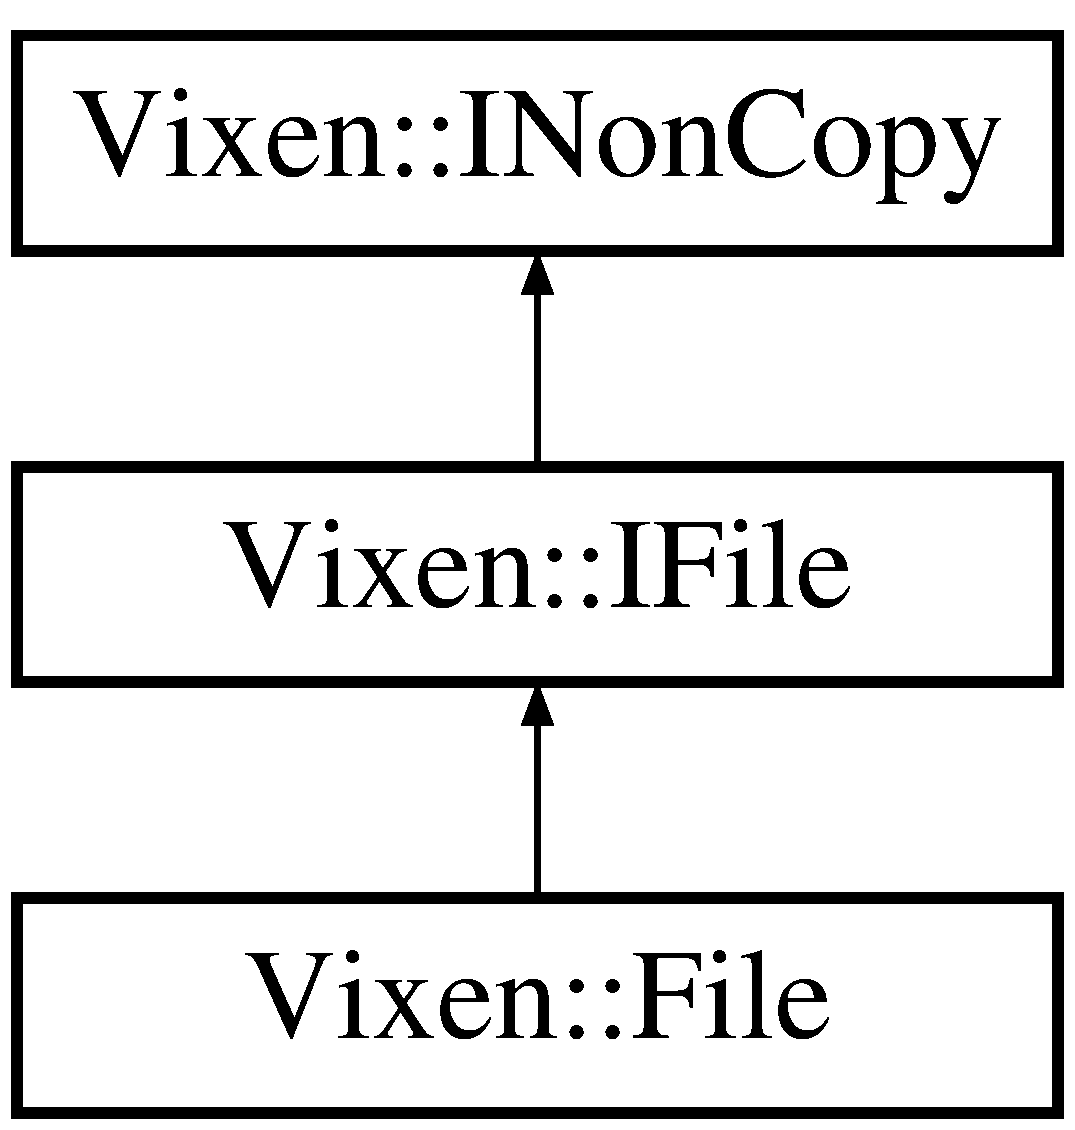
\includegraphics[height=3.000000cm]{classVixen_1_1File}
\end{center}
\end{figure}
\subsection*{Public Member Functions}
\begin{DoxyCompactItemize}
\item 
\hyperlink{classVixen_1_1File_a11603af08d0e41ff25a47d5634d19a41}{File} ()
\item 
\hyperlink{classVixen_1_1File_a1079eded77d83b42fcad7db4f3ad98d8}{$\sim$\+File} (void)
\item 
virtual \hyperlink{namespaceVixen_a28cf3e45633036dc0ae46d5ab701af86}{File\+Error} \hyperlink{classVixen_1_1File_a14ec6c12a37a1f60617bbf9313b24d8f}{Error} ()
\item 
virtual \hyperlink{vix__stringutil_8h_a561c282c415a5c38fd9a26325701e3bf}{U\+String} \hyperlink{classVixen_1_1File_a10b0b7cf7ead8a8936aa22cc1f6b9318}{File\+Name} ()
\item 
virtual \hyperlink{vix__stringutil_8h_a561c282c415a5c38fd9a26325701e3bf}{U\+String} \hyperlink{classVixen_1_1File_a2985c6a6cb9a53f6eef0e125e6885051}{File\+Path} ()
\item 
virtual \hyperlink{vix__stringutil_8h_a561c282c415a5c38fd9a26325701e3bf}{U\+String} \hyperlink{classVixen_1_1File_a55e0c906130d29cf5583503016342ddd}{Base\+Name} ()
\item 
virtual bool \hyperlink{classVixen_1_1File_ac3869f8194a442f31d86122dfa8a3837}{Flush} ()
\item 
virtual bool \hyperlink{classVixen_1_1File_a24d43934cc6c607ebba11596c7429595}{Open} (\hyperlink{vix__stringutil_8h_a561c282c415a5c38fd9a26325701e3bf}{U\+String} path)
\item 
virtual bool \hyperlink{classVixen_1_1File_a4def6de72e2f89dc08c1cd1f0c051bad}{Seek} (size\+\_\+t offset, \hyperlink{namespaceVixen_a3819245066e95e1d70b59a549654e606}{File\+Seek} mode)
\item 
virtual void \hyperlink{classVixen_1_1File_a42e051c2575db0c2a594e18c6f650957}{Read} (\hyperlink{vix__platform_8h_a4ae1dab0fb4b072a66584546209e7d58}{B\+Y\+T\+E} $\ast$out, size\+\_\+t len)
\item 
virtual bool \hyperlink{classVixen_1_1File_a3f1848aba4558bd98714c528c3fe0b73}{Close} ()
\item 
virtual size\+\_\+t \hyperlink{classVixen_1_1File_a3071f337ce92a2a8bcb1470cabc1ca87}{Tell} ()
\item 
virtual size\+\_\+t \hyperlink{classVixen_1_1File_a039eb93e24d180e4dd9779c9667242f0}{Size\+Bytes} ()
\item 
virtual size\+\_\+t \hyperlink{classVixen_1_1File_a5d5bbcc901aacfaeba1c034eedb791df}{Size\+K\+Bytes} ()
\item 
virtual size\+\_\+t \hyperlink{classVixen_1_1File_acdc342b07d6d1f7b11d5b0edcb573ddc}{Position} ()
\item 
virtual F\+I\+L\+E $\ast$ \hyperlink{classVixen_1_1File_a03d0e61e3fe875360cce0bdd639b2893}{Handle} ()
\item 
virtual bool \hyperlink{classVixen_1_1File_a3d03ec3abc2fe10164dead567725fa1f}{P\+Error} (int err=0)
\end{DoxyCompactItemize}
\subsection*{Protected Attributes}
\begin{DoxyCompactItemize}
\item 
\hyperlink{namespaceVixen_a28cf3e45633036dc0ae46d5ab701af86}{File\+Error} \hyperlink{classVixen_1_1File_ab696ed339a9c3f80190ab98602bbd86d}{m\+\_\+error}
\item 
\hyperlink{vix__stringutil_8h_a561c282c415a5c38fd9a26325701e3bf}{U\+String} \hyperlink{classVixen_1_1File_a11693f442d424e458a44b3d5d125f214}{m\+\_\+file\+Path}
\item 
\hyperlink{vix__stringutil_8h_a561c282c415a5c38fd9a26325701e3bf}{U\+String} \hyperlink{classVixen_1_1File_afeaa0bacfeb45b5dd635c23ed27552d9}{m\+\_\+file\+Name}
\item 
\hyperlink{vix__stringutil_8h_a561c282c415a5c38fd9a26325701e3bf}{U\+String} \hyperlink{classVixen_1_1File_abb5e1d86973c517ceada94bd71a54366}{m\+\_\+base\+Name}
\item 
size\+\_\+t \hyperlink{classVixen_1_1File_a5fe4fdd2471edc9ea7d1d0de2ad75d05}{m\+\_\+position}
\item 
size\+\_\+t \hyperlink{classVixen_1_1File_a709d76aebf0a4a81b8fb2940a52780cd}{m\+\_\+size}
\item 
F\+I\+L\+E $\ast$ \hyperlink{classVixen_1_1File_afe1a750718bfda28c1f65508cb59b187}{m\+\_\+handle}
\end{DoxyCompactItemize}
\subsection*{Additional Inherited Members}


\subsection{Constructor \& Destructor Documentation}
\hypertarget{classVixen_1_1File_a11603af08d0e41ff25a47d5634d19a41}{}\index{Vixen\+::\+File@{Vixen\+::\+File}!File@{File}}
\index{File@{File}!Vixen\+::\+File@{Vixen\+::\+File}}
\subsubsection[{File}]{\setlength{\rightskip}{0pt plus 5cm}Vixen\+::\+File\+::\+File (
\begin{DoxyParamCaption}
{}
\end{DoxyParamCaption}
)}\label{classVixen_1_1File_a11603af08d0e41ff25a47d5634d19a41}
\hypertarget{classVixen_1_1File_a1079eded77d83b42fcad7db4f3ad98d8}{}\index{Vixen\+::\+File@{Vixen\+::\+File}!````~File@{$\sim$\+File}}
\index{````~File@{$\sim$\+File}!Vixen\+::\+File@{Vixen\+::\+File}}
\subsubsection[{$\sim$\+File}]{\setlength{\rightskip}{0pt plus 5cm}Vixen\+::\+File\+::$\sim$\+File (
\begin{DoxyParamCaption}
\item[{void}]{}
\end{DoxyParamCaption}
)}\label{classVixen_1_1File_a1079eded77d83b42fcad7db4f3ad98d8}


\subsection{Member Function Documentation}
\hypertarget{classVixen_1_1File_a55e0c906130d29cf5583503016342ddd}{}\index{Vixen\+::\+File@{Vixen\+::\+File}!Base\+Name@{Base\+Name}}
\index{Base\+Name@{Base\+Name}!Vixen\+::\+File@{Vixen\+::\+File}}
\subsubsection[{Base\+Name}]{\setlength{\rightskip}{0pt plus 5cm}{\bf U\+String} Vixen\+::\+File\+::\+Base\+Name (
\begin{DoxyParamCaption}
{}
\end{DoxyParamCaption}
)\hspace{0.3cm}{\ttfamily [virtual]}}\label{classVixen_1_1File_a55e0c906130d29cf5583503016342ddd}


Implements \hyperlink{classVixen_1_1IFile_a5f50dba2f5efaa1b5438b9924dad8d85}{Vixen\+::\+I\+File}.

\hypertarget{classVixen_1_1File_a3f1848aba4558bd98714c528c3fe0b73}{}\index{Vixen\+::\+File@{Vixen\+::\+File}!Close@{Close}}
\index{Close@{Close}!Vixen\+::\+File@{Vixen\+::\+File}}
\subsubsection[{Close}]{\setlength{\rightskip}{0pt plus 5cm}bool Vixen\+::\+File\+::\+Close (
\begin{DoxyParamCaption}
{}
\end{DoxyParamCaption}
)\hspace{0.3cm}{\ttfamily [virtual]}}\label{classVixen_1_1File_a3f1848aba4558bd98714c528c3fe0b73}


Implements \hyperlink{classVixen_1_1IFile_ae22fba81f1a450f94bbaa993e342d28b}{Vixen\+::\+I\+File}.

\hypertarget{classVixen_1_1File_a14ec6c12a37a1f60617bbf9313b24d8f}{}\index{Vixen\+::\+File@{Vixen\+::\+File}!Error@{Error}}
\index{Error@{Error}!Vixen\+::\+File@{Vixen\+::\+File}}
\subsubsection[{Error}]{\setlength{\rightskip}{0pt plus 5cm}{\bf File\+Error} Vixen\+::\+File\+::\+Error (
\begin{DoxyParamCaption}
{}
\end{DoxyParamCaption}
)\hspace{0.3cm}{\ttfamily [virtual]}}\label{classVixen_1_1File_a14ec6c12a37a1f60617bbf9313b24d8f}


Implements \hyperlink{classVixen_1_1IFile_a5918065a61d316d170d5b20f46a7a770}{Vixen\+::\+I\+File}.

\hypertarget{classVixen_1_1File_a10b0b7cf7ead8a8936aa22cc1f6b9318}{}\index{Vixen\+::\+File@{Vixen\+::\+File}!File\+Name@{File\+Name}}
\index{File\+Name@{File\+Name}!Vixen\+::\+File@{Vixen\+::\+File}}
\subsubsection[{File\+Name}]{\setlength{\rightskip}{0pt plus 5cm}{\bf U\+String} Vixen\+::\+File\+::\+File\+Name (
\begin{DoxyParamCaption}
{}
\end{DoxyParamCaption}
)\hspace{0.3cm}{\ttfamily [virtual]}}\label{classVixen_1_1File_a10b0b7cf7ead8a8936aa22cc1f6b9318}


Implements \hyperlink{classVixen_1_1IFile_a23244672c3e59af8dfdfd77fe6df992b}{Vixen\+::\+I\+File}.

\hypertarget{classVixen_1_1File_a2985c6a6cb9a53f6eef0e125e6885051}{}\index{Vixen\+::\+File@{Vixen\+::\+File}!File\+Path@{File\+Path}}
\index{File\+Path@{File\+Path}!Vixen\+::\+File@{Vixen\+::\+File}}
\subsubsection[{File\+Path}]{\setlength{\rightskip}{0pt plus 5cm}{\bf U\+String} Vixen\+::\+File\+::\+File\+Path (
\begin{DoxyParamCaption}
{}
\end{DoxyParamCaption}
)\hspace{0.3cm}{\ttfamily [virtual]}}\label{classVixen_1_1File_a2985c6a6cb9a53f6eef0e125e6885051}


Implements \hyperlink{classVixen_1_1IFile_aed9fd463648dbd5a5de9310711e9206b}{Vixen\+::\+I\+File}.

\hypertarget{classVixen_1_1File_ac3869f8194a442f31d86122dfa8a3837}{}\index{Vixen\+::\+File@{Vixen\+::\+File}!Flush@{Flush}}
\index{Flush@{Flush}!Vixen\+::\+File@{Vixen\+::\+File}}
\subsubsection[{Flush}]{\setlength{\rightskip}{0pt plus 5cm}bool Vixen\+::\+File\+::\+Flush (
\begin{DoxyParamCaption}
{}
\end{DoxyParamCaption}
)\hspace{0.3cm}{\ttfamily [virtual]}}\label{classVixen_1_1File_ac3869f8194a442f31d86122dfa8a3837}


Implements \hyperlink{classVixen_1_1IFile_a64d455adfd53b5395ced42605aa77186}{Vixen\+::\+I\+File}.

\hypertarget{classVixen_1_1File_a03d0e61e3fe875360cce0bdd639b2893}{}\index{Vixen\+::\+File@{Vixen\+::\+File}!Handle@{Handle}}
\index{Handle@{Handle}!Vixen\+::\+File@{Vixen\+::\+File}}
\subsubsection[{Handle}]{\setlength{\rightskip}{0pt plus 5cm}F\+I\+L\+E $\ast$ Vixen\+::\+File\+::\+Handle (
\begin{DoxyParamCaption}
{}
\end{DoxyParamCaption}
)\hspace{0.3cm}{\ttfamily [virtual]}}\label{classVixen_1_1File_a03d0e61e3fe875360cce0bdd639b2893}


Implements \hyperlink{classVixen_1_1IFile_a94e965cd24ea950f98f269317df6f010}{Vixen\+::\+I\+File}.

\hypertarget{classVixen_1_1File_a24d43934cc6c607ebba11596c7429595}{}\index{Vixen\+::\+File@{Vixen\+::\+File}!Open@{Open}}
\index{Open@{Open}!Vixen\+::\+File@{Vixen\+::\+File}}
\subsubsection[{Open}]{\setlength{\rightskip}{0pt plus 5cm}bool Vixen\+::\+File\+::\+Open (
\begin{DoxyParamCaption}
\item[{{\bf U\+String}}]{path}
\end{DoxyParamCaption}
)\hspace{0.3cm}{\ttfamily [virtual]}}\label{classVixen_1_1File_a24d43934cc6c607ebba11596c7429595}


Implements \hyperlink{classVixen_1_1IFile_a719f5df723010adfcaaf2ef6fc02e414}{Vixen\+::\+I\+File}.

\hypertarget{classVixen_1_1File_a3d03ec3abc2fe10164dead567725fa1f}{}\index{Vixen\+::\+File@{Vixen\+::\+File}!P\+Error@{P\+Error}}
\index{P\+Error@{P\+Error}!Vixen\+::\+File@{Vixen\+::\+File}}
\subsubsection[{P\+Error}]{\setlength{\rightskip}{0pt plus 5cm}bool Vixen\+::\+File\+::\+P\+Error (
\begin{DoxyParamCaption}
\item[{int}]{err = {\ttfamily 0}}
\end{DoxyParamCaption}
)\hspace{0.3cm}{\ttfamily [virtual]}}\label{classVixen_1_1File_a3d03ec3abc2fe10164dead567725fa1f}


Implements \hyperlink{classVixen_1_1IFile_aec62be3125fd105bdf059e15b4cd4603}{Vixen\+::\+I\+File}.

\hypertarget{classVixen_1_1File_acdc342b07d6d1f7b11d5b0edcb573ddc}{}\index{Vixen\+::\+File@{Vixen\+::\+File}!Position@{Position}}
\index{Position@{Position}!Vixen\+::\+File@{Vixen\+::\+File}}
\subsubsection[{Position}]{\setlength{\rightskip}{0pt plus 5cm}size\+\_\+t Vixen\+::\+File\+::\+Position (
\begin{DoxyParamCaption}
{}
\end{DoxyParamCaption}
)\hspace{0.3cm}{\ttfamily [virtual]}}\label{classVixen_1_1File_acdc342b07d6d1f7b11d5b0edcb573ddc}


Implements \hyperlink{classVixen_1_1IFile_a1ca999110df6a5a71bb07f374df5f722}{Vixen\+::\+I\+File}.

\hypertarget{classVixen_1_1File_a42e051c2575db0c2a594e18c6f650957}{}\index{Vixen\+::\+File@{Vixen\+::\+File}!Read@{Read}}
\index{Read@{Read}!Vixen\+::\+File@{Vixen\+::\+File}}
\subsubsection[{Read}]{\setlength{\rightskip}{0pt plus 5cm}void Vixen\+::\+File\+::\+Read (
\begin{DoxyParamCaption}
\item[{{\bf B\+Y\+T\+E} $\ast$}]{out, }
\item[{size\+\_\+t}]{len}
\end{DoxyParamCaption}
)\hspace{0.3cm}{\ttfamily [virtual]}}\label{classVixen_1_1File_a42e051c2575db0c2a594e18c6f650957}


Implements \hyperlink{classVixen_1_1IFile_a4dd88412328626d860870edb22c01d34}{Vixen\+::\+I\+File}.

\hypertarget{classVixen_1_1File_a4def6de72e2f89dc08c1cd1f0c051bad}{}\index{Vixen\+::\+File@{Vixen\+::\+File}!Seek@{Seek}}
\index{Seek@{Seek}!Vixen\+::\+File@{Vixen\+::\+File}}
\subsubsection[{Seek}]{\setlength{\rightskip}{0pt plus 5cm}bool Vixen\+::\+File\+::\+Seek (
\begin{DoxyParamCaption}
\item[{size\+\_\+t}]{offset, }
\item[{{\bf File\+Seek}}]{mode}
\end{DoxyParamCaption}
)\hspace{0.3cm}{\ttfamily [virtual]}}\label{classVixen_1_1File_a4def6de72e2f89dc08c1cd1f0c051bad}


Implements \hyperlink{classVixen_1_1IFile_af1ebf5771acc6e8553797614de65dfd2}{Vixen\+::\+I\+File}.

\hypertarget{classVixen_1_1File_a039eb93e24d180e4dd9779c9667242f0}{}\index{Vixen\+::\+File@{Vixen\+::\+File}!Size\+Bytes@{Size\+Bytes}}
\index{Size\+Bytes@{Size\+Bytes}!Vixen\+::\+File@{Vixen\+::\+File}}
\subsubsection[{Size\+Bytes}]{\setlength{\rightskip}{0pt plus 5cm}size\+\_\+t Vixen\+::\+File\+::\+Size\+Bytes (
\begin{DoxyParamCaption}
{}
\end{DoxyParamCaption}
)\hspace{0.3cm}{\ttfamily [virtual]}}\label{classVixen_1_1File_a039eb93e24d180e4dd9779c9667242f0}


Implements \hyperlink{classVixen_1_1IFile_ade8c8d3e40bebf52130c23a0bace4db8}{Vixen\+::\+I\+File}.

\hypertarget{classVixen_1_1File_a5d5bbcc901aacfaeba1c034eedb791df}{}\index{Vixen\+::\+File@{Vixen\+::\+File}!Size\+K\+Bytes@{Size\+K\+Bytes}}
\index{Size\+K\+Bytes@{Size\+K\+Bytes}!Vixen\+::\+File@{Vixen\+::\+File}}
\subsubsection[{Size\+K\+Bytes}]{\setlength{\rightskip}{0pt plus 5cm}size\+\_\+t Vixen\+::\+File\+::\+Size\+K\+Bytes (
\begin{DoxyParamCaption}
{}
\end{DoxyParamCaption}
)\hspace{0.3cm}{\ttfamily [virtual]}}\label{classVixen_1_1File_a5d5bbcc901aacfaeba1c034eedb791df}


Implements \hyperlink{classVixen_1_1IFile_aafcb6f019831af8743e5a28fb2753126}{Vixen\+::\+I\+File}.

\hypertarget{classVixen_1_1File_a3071f337ce92a2a8bcb1470cabc1ca87}{}\index{Vixen\+::\+File@{Vixen\+::\+File}!Tell@{Tell}}
\index{Tell@{Tell}!Vixen\+::\+File@{Vixen\+::\+File}}
\subsubsection[{Tell}]{\setlength{\rightskip}{0pt plus 5cm}size\+\_\+t Vixen\+::\+File\+::\+Tell (
\begin{DoxyParamCaption}
{}
\end{DoxyParamCaption}
)\hspace{0.3cm}{\ttfamily [virtual]}}\label{classVixen_1_1File_a3071f337ce92a2a8bcb1470cabc1ca87}


Implements \hyperlink{classVixen_1_1IFile_a473b1cfa328219a5f85d745fe7f33ebd}{Vixen\+::\+I\+File}.



\subsection{Member Data Documentation}
\hypertarget{classVixen_1_1File_abb5e1d86973c517ceada94bd71a54366}{}\index{Vixen\+::\+File@{Vixen\+::\+File}!m\+\_\+base\+Name@{m\+\_\+base\+Name}}
\index{m\+\_\+base\+Name@{m\+\_\+base\+Name}!Vixen\+::\+File@{Vixen\+::\+File}}
\subsubsection[{m\+\_\+base\+Name}]{\setlength{\rightskip}{0pt plus 5cm}{\bf U\+String} Vixen\+::\+File\+::m\+\_\+base\+Name\hspace{0.3cm}{\ttfamily [protected]}}\label{classVixen_1_1File_abb5e1d86973c517ceada94bd71a54366}
\hypertarget{classVixen_1_1File_ab696ed339a9c3f80190ab98602bbd86d}{}\index{Vixen\+::\+File@{Vixen\+::\+File}!m\+\_\+error@{m\+\_\+error}}
\index{m\+\_\+error@{m\+\_\+error}!Vixen\+::\+File@{Vixen\+::\+File}}
\subsubsection[{m\+\_\+error}]{\setlength{\rightskip}{0pt plus 5cm}{\bf File\+Error} Vixen\+::\+File\+::m\+\_\+error\hspace{0.3cm}{\ttfamily [protected]}}\label{classVixen_1_1File_ab696ed339a9c3f80190ab98602bbd86d}
\hypertarget{classVixen_1_1File_afeaa0bacfeb45b5dd635c23ed27552d9}{}\index{Vixen\+::\+File@{Vixen\+::\+File}!m\+\_\+file\+Name@{m\+\_\+file\+Name}}
\index{m\+\_\+file\+Name@{m\+\_\+file\+Name}!Vixen\+::\+File@{Vixen\+::\+File}}
\subsubsection[{m\+\_\+file\+Name}]{\setlength{\rightskip}{0pt plus 5cm}{\bf U\+String} Vixen\+::\+File\+::m\+\_\+file\+Name\hspace{0.3cm}{\ttfamily [protected]}}\label{classVixen_1_1File_afeaa0bacfeb45b5dd635c23ed27552d9}
\hypertarget{classVixen_1_1File_a11693f442d424e458a44b3d5d125f214}{}\index{Vixen\+::\+File@{Vixen\+::\+File}!m\+\_\+file\+Path@{m\+\_\+file\+Path}}
\index{m\+\_\+file\+Path@{m\+\_\+file\+Path}!Vixen\+::\+File@{Vixen\+::\+File}}
\subsubsection[{m\+\_\+file\+Path}]{\setlength{\rightskip}{0pt plus 5cm}{\bf U\+String} Vixen\+::\+File\+::m\+\_\+file\+Path\hspace{0.3cm}{\ttfamily [protected]}}\label{classVixen_1_1File_a11693f442d424e458a44b3d5d125f214}
\hypertarget{classVixen_1_1File_afe1a750718bfda28c1f65508cb59b187}{}\index{Vixen\+::\+File@{Vixen\+::\+File}!m\+\_\+handle@{m\+\_\+handle}}
\index{m\+\_\+handle@{m\+\_\+handle}!Vixen\+::\+File@{Vixen\+::\+File}}
\subsubsection[{m\+\_\+handle}]{\setlength{\rightskip}{0pt plus 5cm}F\+I\+L\+E$\ast$ Vixen\+::\+File\+::m\+\_\+handle\hspace{0.3cm}{\ttfamily [protected]}}\label{classVixen_1_1File_afe1a750718bfda28c1f65508cb59b187}
\hypertarget{classVixen_1_1File_a5fe4fdd2471edc9ea7d1d0de2ad75d05}{}\index{Vixen\+::\+File@{Vixen\+::\+File}!m\+\_\+position@{m\+\_\+position}}
\index{m\+\_\+position@{m\+\_\+position}!Vixen\+::\+File@{Vixen\+::\+File}}
\subsubsection[{m\+\_\+position}]{\setlength{\rightskip}{0pt plus 5cm}size\+\_\+t Vixen\+::\+File\+::m\+\_\+position\hspace{0.3cm}{\ttfamily [protected]}}\label{classVixen_1_1File_a5fe4fdd2471edc9ea7d1d0de2ad75d05}
\hypertarget{classVixen_1_1File_a709d76aebf0a4a81b8fb2940a52780cd}{}\index{Vixen\+::\+File@{Vixen\+::\+File}!m\+\_\+size@{m\+\_\+size}}
\index{m\+\_\+size@{m\+\_\+size}!Vixen\+::\+File@{Vixen\+::\+File}}
\subsubsection[{m\+\_\+size}]{\setlength{\rightskip}{0pt plus 5cm}size\+\_\+t Vixen\+::\+File\+::m\+\_\+size\hspace{0.3cm}{\ttfamily [protected]}}\label{classVixen_1_1File_a709d76aebf0a4a81b8fb2940a52780cd}


The documentation for this class was generated from the following files\+:\begin{DoxyCompactItemize}
\item 
/home/debunez/\+Development/\+Vixen\+Engine/include/vcore/\hyperlink{vix__file_8h}{vix\+\_\+file.\+h}\item 
/home/debunez/\+Development/\+Vixen\+Engine/source/vcore/\hyperlink{vix__file_8cpp}{vix\+\_\+file.\+cpp}\end{DoxyCompactItemize}

\hypertarget{classVixen_1_1FileManager}{}\section{Vixen\+:\+:File\+Manager Class Reference}
\label{classVixen_1_1FileManager}\index{Vixen\+::\+File\+Manager@{Vixen\+::\+File\+Manager}}


{\ttfamily \#include $<$vix\+\_\+filemanager.\+h$>$}

Inheritance diagram for Vixen\+:\+:File\+Manager\+:\begin{figure}[H]
\begin{center}
\leavevmode
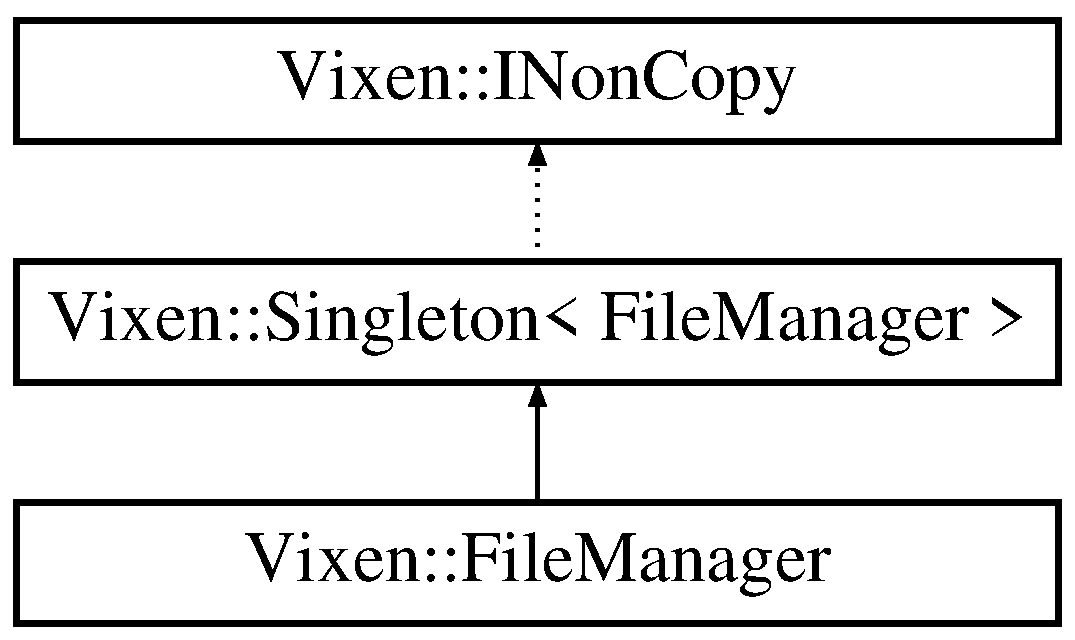
\includegraphics[height=3.000000cm]{classVixen_1_1FileManager}
\end{center}
\end{figure}
\subsection*{Public Member Functions}
\begin{DoxyCompactItemize}
\item 
\hyperlink{classVixen_1_1FileManager_abdbeed26d1b9d2014b5b735365c3fecb}{$\sim$\+File\+Manager} ()
\end{DoxyCompactItemize}
\subsection*{Static Public Member Functions}
\begin{DoxyCompactItemize}
\item 
static void \hyperlink{classVixen_1_1FileManager_a3c93be5972cbc9a8460d6177bff29e58}{Open\+File} (\hyperlink{vix__stringutil_8h_a561c282c415a5c38fd9a26325701e3bf}{U\+String} file\+Path)
\item 
static void \hyperlink{classVixen_1_1FileManager_a36342248ec7f83ff8917a6a210707266}{Close\+File} (\hyperlink{vix__stringutil_8h_a561c282c415a5c38fd9a26325701e3bf}{U\+String} file\+Path)
\item 
static \hyperlink{classVixen_1_1File}{File} $\ast$ \hyperlink{classVixen_1_1FileManager_a6f2939cb810556b9cc6ef63b0f7131e8}{Access\+File} (\hyperlink{vix__stringutil_8h_a561c282c415a5c38fd9a26325701e3bf}{U\+String} file\+Path)
\end{DoxyCompactItemize}
\subsection*{Additional Inherited Members}


\subsection{Constructor \& Destructor Documentation}
\hypertarget{classVixen_1_1FileManager_abdbeed26d1b9d2014b5b735365c3fecb}{}\index{Vixen\+::\+File\+Manager@{Vixen\+::\+File\+Manager}!````~File\+Manager@{$\sim$\+File\+Manager}}
\index{````~File\+Manager@{$\sim$\+File\+Manager}!Vixen\+::\+File\+Manager@{Vixen\+::\+File\+Manager}}
\subsubsection[{$\sim$\+File\+Manager}]{\setlength{\rightskip}{0pt plus 5cm}Vixen\+::\+File\+Manager\+::$\sim$\+File\+Manager (
\begin{DoxyParamCaption}
{}
\end{DoxyParamCaption}
)}\label{classVixen_1_1FileManager_abdbeed26d1b9d2014b5b735365c3fecb}


\subsection{Member Function Documentation}
\hypertarget{classVixen_1_1FileManager_a6f2939cb810556b9cc6ef63b0f7131e8}{}\index{Vixen\+::\+File\+Manager@{Vixen\+::\+File\+Manager}!Access\+File@{Access\+File}}
\index{Access\+File@{Access\+File}!Vixen\+::\+File\+Manager@{Vixen\+::\+File\+Manager}}
\subsubsection[{Access\+File}]{\setlength{\rightskip}{0pt plus 5cm}{\bf File} $\ast$ Vixen\+::\+File\+Manager\+::\+Access\+File (
\begin{DoxyParamCaption}
\item[{{\bf U\+String}}]{file\+Path}
\end{DoxyParamCaption}
)\hspace{0.3cm}{\ttfamily [static]}}\label{classVixen_1_1FileManager_a6f2939cb810556b9cc6ef63b0f7131e8}
\hypertarget{classVixen_1_1FileManager_a36342248ec7f83ff8917a6a210707266}{}\index{Vixen\+::\+File\+Manager@{Vixen\+::\+File\+Manager}!Close\+File@{Close\+File}}
\index{Close\+File@{Close\+File}!Vixen\+::\+File\+Manager@{Vixen\+::\+File\+Manager}}
\subsubsection[{Close\+File}]{\setlength{\rightskip}{0pt plus 5cm}void Vixen\+::\+File\+Manager\+::\+Close\+File (
\begin{DoxyParamCaption}
\item[{{\bf U\+String}}]{file\+Path}
\end{DoxyParamCaption}
)\hspace{0.3cm}{\ttfamily [static]}}\label{classVixen_1_1FileManager_a36342248ec7f83ff8917a6a210707266}
\hypertarget{classVixen_1_1FileManager_a3c93be5972cbc9a8460d6177bff29e58}{}\index{Vixen\+::\+File\+Manager@{Vixen\+::\+File\+Manager}!Open\+File@{Open\+File}}
\index{Open\+File@{Open\+File}!Vixen\+::\+File\+Manager@{Vixen\+::\+File\+Manager}}
\subsubsection[{Open\+File}]{\setlength{\rightskip}{0pt plus 5cm}void Vixen\+::\+File\+Manager\+::\+Open\+File (
\begin{DoxyParamCaption}
\item[{{\bf U\+String}}]{file\+Path}
\end{DoxyParamCaption}
)\hspace{0.3cm}{\ttfamily [static]}}\label{classVixen_1_1FileManager_a3c93be5972cbc9a8460d6177bff29e58}


The documentation for this class was generated from the following files\+:\begin{DoxyCompactItemize}
\item 
/home/debunez/\+Development/\+Vixen\+Engine/include/vcore/\hyperlink{vix__filemanager_8h}{vix\+\_\+filemanager.\+h}\item 
/home/debunez/\+Development/\+Vixen\+Engine/source/vcore/\hyperlink{vix__filemanager_8cpp}{vix\+\_\+filemanager.\+cpp}\end{DoxyCompactItemize}

\hypertarget{classVixen_1_1IContent}{}\section{Vixen\+:\+:I\+Content Class Reference}
\label{classVixen_1_1IContent}\index{Vixen\+::\+I\+Content@{Vixen\+::\+I\+Content}}


{\ttfamily \#include $<$vix\+\_\+content.\+h$>$}



The documentation for this class was generated from the following file\+:\begin{DoxyCompactItemize}
\item 
/home/debunez/\+Development/\+Vixen\+Engine/include/vcore/\hyperlink{vix__content_8h}{vix\+\_\+content.\+h}\end{DoxyCompactItemize}

\hypertarget{classVixen_1_1IFile}{}\section{Vixen\+:\+:I\+File Class Reference}
\label{classVixen_1_1IFile}\index{Vixen\+::\+I\+File@{Vixen\+::\+I\+File}}


{\ttfamily \#include $<$vix\+\_\+file\+\_\+interface.\+h$>$}

Inheritance diagram for Vixen\+:\+:I\+File\+:\begin{figure}[H]
\begin{center}
\leavevmode
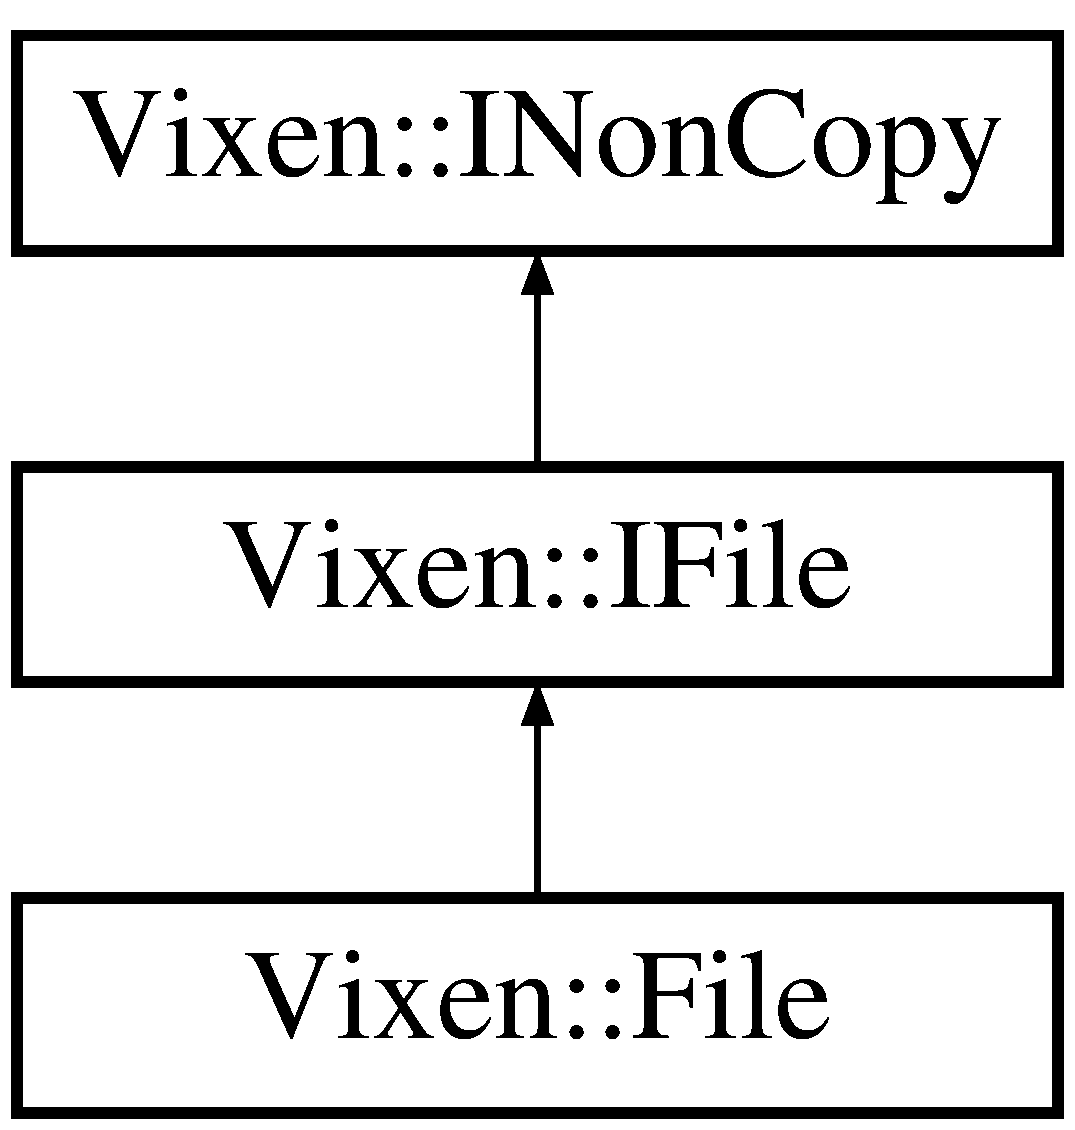
\includegraphics[height=3.000000cm]{classVixen_1_1IFile}
\end{center}
\end{figure}
\subsection*{Public Member Functions}
\begin{DoxyCompactItemize}
\item 
virtual \hyperlink{classVixen_1_1IFile_aedecb0b2d638fdfa33ad9fb8890ccbc6}{$\sim$\+I\+File} ()
\item 
virtual \hyperlink{namespaceVixen_a28cf3e45633036dc0ae46d5ab701af86}{File\+Error} \hyperlink{classVixen_1_1IFile_a5918065a61d316d170d5b20f46a7a770}{Error} ()=0
\item 
virtual \hyperlink{vix__stringutil_8h_a561c282c415a5c38fd9a26325701e3bf}{U\+String} \hyperlink{classVixen_1_1IFile_a23244672c3e59af8dfdfd77fe6df992b}{File\+Name} ()=0
\item 
virtual \hyperlink{vix__stringutil_8h_a561c282c415a5c38fd9a26325701e3bf}{U\+String} \hyperlink{classVixen_1_1IFile_aed9fd463648dbd5a5de9310711e9206b}{File\+Path} ()=0
\item 
virtual \hyperlink{vix__stringutil_8h_a561c282c415a5c38fd9a26325701e3bf}{U\+String} \hyperlink{classVixen_1_1IFile_a5f50dba2f5efaa1b5438b9924dad8d85}{Base\+Name} ()=0
\item 
virtual bool \hyperlink{classVixen_1_1IFile_a719f5df723010adfcaaf2ef6fc02e414}{Open} (\hyperlink{vix__stringutil_8h_a561c282c415a5c38fd9a26325701e3bf}{U\+String} path)=0
\item 
virtual bool \hyperlink{classVixen_1_1IFile_a64d455adfd53b5395ced42605aa77186}{Flush} ()=0
\item 
virtual bool \hyperlink{classVixen_1_1IFile_af1ebf5771acc6e8553797614de65dfd2}{Seek} (size\+\_\+t offset, \hyperlink{namespaceVixen_a3819245066e95e1d70b59a549654e606}{File\+Seek} mode)=0
\item 
virtual bool \hyperlink{classVixen_1_1IFile_ae22fba81f1a450f94bbaa993e342d28b}{Close} ()=0
\item 
virtual void \hyperlink{classVixen_1_1IFile_a4dd88412328626d860870edb22c01d34}{Read} (\hyperlink{vix__platform_8h_a4ae1dab0fb4b072a66584546209e7d58}{B\+Y\+T\+E} $\ast$out, size\+\_\+t len)=0
\item 
virtual size\+\_\+t \hyperlink{classVixen_1_1IFile_a473b1cfa328219a5f85d745fe7f33ebd}{Tell} ()=0
\item 
virtual size\+\_\+t \hyperlink{classVixen_1_1IFile_ade8c8d3e40bebf52130c23a0bace4db8}{Size\+Bytes} ()=0
\item 
virtual size\+\_\+t \hyperlink{classVixen_1_1IFile_aafcb6f019831af8743e5a28fb2753126}{Size\+K\+Bytes} ()=0
\item 
virtual size\+\_\+t \hyperlink{classVixen_1_1IFile_a1ca999110df6a5a71bb07f374df5f722}{Position} ()=0
\item 
virtual F\+I\+L\+E $\ast$ \hyperlink{classVixen_1_1IFile_a94e965cd24ea950f98f269317df6f010}{Handle} ()=0
\item 
virtual bool \hyperlink{classVixen_1_1IFile_aec62be3125fd105bdf059e15b4cd4603}{P\+Error} (int err=0)=0
\end{DoxyCompactItemize}
\subsection*{Additional Inherited Members}


\subsection{Detailed Description}
I\+F\+Ile interface

Describes base class of all \hyperlink{classVixen_1_1File}{File} I/\+O classes 

\subsection{Constructor \& Destructor Documentation}
\hypertarget{classVixen_1_1IFile_aedecb0b2d638fdfa33ad9fb8890ccbc6}{}\index{Vixen\+::\+I\+File@{Vixen\+::\+I\+File}!````~I\+File@{$\sim$\+I\+File}}
\index{````~I\+File@{$\sim$\+I\+File}!Vixen\+::\+I\+File@{Vixen\+::\+I\+File}}
\subsubsection[{$\sim$\+I\+File}]{\setlength{\rightskip}{0pt plus 5cm}virtual Vixen\+::\+I\+File\+::$\sim$\+I\+File (
\begin{DoxyParamCaption}
{}
\end{DoxyParamCaption}
)\hspace{0.3cm}{\ttfamily [inline]}, {\ttfamily [virtual]}}\label{classVixen_1_1IFile_aedecb0b2d638fdfa33ad9fb8890ccbc6}


\subsection{Member Function Documentation}
\hypertarget{classVixen_1_1IFile_a5f50dba2f5efaa1b5438b9924dad8d85}{}\index{Vixen\+::\+I\+File@{Vixen\+::\+I\+File}!Base\+Name@{Base\+Name}}
\index{Base\+Name@{Base\+Name}!Vixen\+::\+I\+File@{Vixen\+::\+I\+File}}
\subsubsection[{Base\+Name}]{\setlength{\rightskip}{0pt plus 5cm}virtual {\bf U\+String} Vixen\+::\+I\+File\+::\+Base\+Name (
\begin{DoxyParamCaption}
{}
\end{DoxyParamCaption}
)\hspace{0.3cm}{\ttfamily [pure virtual]}}\label{classVixen_1_1IFile_a5f50dba2f5efaa1b5438b9924dad8d85}


Implemented in \hyperlink{classVixen_1_1File_a55e0c906130d29cf5583503016342ddd}{Vixen\+::\+File}.

\hypertarget{classVixen_1_1IFile_ae22fba81f1a450f94bbaa993e342d28b}{}\index{Vixen\+::\+I\+File@{Vixen\+::\+I\+File}!Close@{Close}}
\index{Close@{Close}!Vixen\+::\+I\+File@{Vixen\+::\+I\+File}}
\subsubsection[{Close}]{\setlength{\rightskip}{0pt plus 5cm}virtual bool Vixen\+::\+I\+File\+::\+Close (
\begin{DoxyParamCaption}
{}
\end{DoxyParamCaption}
)\hspace{0.3cm}{\ttfamily [pure virtual]}}\label{classVixen_1_1IFile_ae22fba81f1a450f94bbaa993e342d28b}


Implemented in \hyperlink{classVixen_1_1File_a3f1848aba4558bd98714c528c3fe0b73}{Vixen\+::\+File}.

\hypertarget{classVixen_1_1IFile_a5918065a61d316d170d5b20f46a7a770}{}\index{Vixen\+::\+I\+File@{Vixen\+::\+I\+File}!Error@{Error}}
\index{Error@{Error}!Vixen\+::\+I\+File@{Vixen\+::\+I\+File}}
\subsubsection[{Error}]{\setlength{\rightskip}{0pt plus 5cm}virtual {\bf File\+Error} Vixen\+::\+I\+File\+::\+Error (
\begin{DoxyParamCaption}
{}
\end{DoxyParamCaption}
)\hspace{0.3cm}{\ttfamily [pure virtual]}}\label{classVixen_1_1IFile_a5918065a61d316d170d5b20f46a7a770}


Implemented in \hyperlink{classVixen_1_1File_a14ec6c12a37a1f60617bbf9313b24d8f}{Vixen\+::\+File}.

\hypertarget{classVixen_1_1IFile_a23244672c3e59af8dfdfd77fe6df992b}{}\index{Vixen\+::\+I\+File@{Vixen\+::\+I\+File}!File\+Name@{File\+Name}}
\index{File\+Name@{File\+Name}!Vixen\+::\+I\+File@{Vixen\+::\+I\+File}}
\subsubsection[{File\+Name}]{\setlength{\rightskip}{0pt plus 5cm}virtual {\bf U\+String} Vixen\+::\+I\+File\+::\+File\+Name (
\begin{DoxyParamCaption}
{}
\end{DoxyParamCaption}
)\hspace{0.3cm}{\ttfamily [pure virtual]}}\label{classVixen_1_1IFile_a23244672c3e59af8dfdfd77fe6df992b}


Implemented in \hyperlink{classVixen_1_1File_a10b0b7cf7ead8a8936aa22cc1f6b9318}{Vixen\+::\+File}.

\hypertarget{classVixen_1_1IFile_aed9fd463648dbd5a5de9310711e9206b}{}\index{Vixen\+::\+I\+File@{Vixen\+::\+I\+File}!File\+Path@{File\+Path}}
\index{File\+Path@{File\+Path}!Vixen\+::\+I\+File@{Vixen\+::\+I\+File}}
\subsubsection[{File\+Path}]{\setlength{\rightskip}{0pt plus 5cm}virtual {\bf U\+String} Vixen\+::\+I\+File\+::\+File\+Path (
\begin{DoxyParamCaption}
{}
\end{DoxyParamCaption}
)\hspace{0.3cm}{\ttfamily [pure virtual]}}\label{classVixen_1_1IFile_aed9fd463648dbd5a5de9310711e9206b}


Implemented in \hyperlink{classVixen_1_1File_a2985c6a6cb9a53f6eef0e125e6885051}{Vixen\+::\+File}.

\hypertarget{classVixen_1_1IFile_a64d455adfd53b5395ced42605aa77186}{}\index{Vixen\+::\+I\+File@{Vixen\+::\+I\+File}!Flush@{Flush}}
\index{Flush@{Flush}!Vixen\+::\+I\+File@{Vixen\+::\+I\+File}}
\subsubsection[{Flush}]{\setlength{\rightskip}{0pt plus 5cm}virtual bool Vixen\+::\+I\+File\+::\+Flush (
\begin{DoxyParamCaption}
{}
\end{DoxyParamCaption}
)\hspace{0.3cm}{\ttfamily [pure virtual]}}\label{classVixen_1_1IFile_a64d455adfd53b5395ced42605aa77186}


Implemented in \hyperlink{classVixen_1_1File_ac3869f8194a442f31d86122dfa8a3837}{Vixen\+::\+File}.

\hypertarget{classVixen_1_1IFile_a94e965cd24ea950f98f269317df6f010}{}\index{Vixen\+::\+I\+File@{Vixen\+::\+I\+File}!Handle@{Handle}}
\index{Handle@{Handle}!Vixen\+::\+I\+File@{Vixen\+::\+I\+File}}
\subsubsection[{Handle}]{\setlength{\rightskip}{0pt plus 5cm}virtual F\+I\+L\+E$\ast$ Vixen\+::\+I\+File\+::\+Handle (
\begin{DoxyParamCaption}
{}
\end{DoxyParamCaption}
)\hspace{0.3cm}{\ttfamily [pure virtual]}}\label{classVixen_1_1IFile_a94e965cd24ea950f98f269317df6f010}


Implemented in \hyperlink{classVixen_1_1File_a03d0e61e3fe875360cce0bdd639b2893}{Vixen\+::\+File}.

\hypertarget{classVixen_1_1IFile_a719f5df723010adfcaaf2ef6fc02e414}{}\index{Vixen\+::\+I\+File@{Vixen\+::\+I\+File}!Open@{Open}}
\index{Open@{Open}!Vixen\+::\+I\+File@{Vixen\+::\+I\+File}}
\subsubsection[{Open}]{\setlength{\rightskip}{0pt plus 5cm}virtual bool Vixen\+::\+I\+File\+::\+Open (
\begin{DoxyParamCaption}
\item[{{\bf U\+String}}]{path}
\end{DoxyParamCaption}
)\hspace{0.3cm}{\ttfamily [pure virtual]}}\label{classVixen_1_1IFile_a719f5df723010adfcaaf2ef6fc02e414}


Implemented in \hyperlink{classVixen_1_1File_a24d43934cc6c607ebba11596c7429595}{Vixen\+::\+File}.

\hypertarget{classVixen_1_1IFile_aec62be3125fd105bdf059e15b4cd4603}{}\index{Vixen\+::\+I\+File@{Vixen\+::\+I\+File}!P\+Error@{P\+Error}}
\index{P\+Error@{P\+Error}!Vixen\+::\+I\+File@{Vixen\+::\+I\+File}}
\subsubsection[{P\+Error}]{\setlength{\rightskip}{0pt plus 5cm}virtual bool Vixen\+::\+I\+File\+::\+P\+Error (
\begin{DoxyParamCaption}
\item[{int}]{err = {\ttfamily 0}}
\end{DoxyParamCaption}
)\hspace{0.3cm}{\ttfamily [pure virtual]}}\label{classVixen_1_1IFile_aec62be3125fd105bdf059e15b4cd4603}


Implemented in \hyperlink{classVixen_1_1File_a3d03ec3abc2fe10164dead567725fa1f}{Vixen\+::\+File}.

\hypertarget{classVixen_1_1IFile_a1ca999110df6a5a71bb07f374df5f722}{}\index{Vixen\+::\+I\+File@{Vixen\+::\+I\+File}!Position@{Position}}
\index{Position@{Position}!Vixen\+::\+I\+File@{Vixen\+::\+I\+File}}
\subsubsection[{Position}]{\setlength{\rightskip}{0pt plus 5cm}virtual size\+\_\+t Vixen\+::\+I\+File\+::\+Position (
\begin{DoxyParamCaption}
{}
\end{DoxyParamCaption}
)\hspace{0.3cm}{\ttfamily [pure virtual]}}\label{classVixen_1_1IFile_a1ca999110df6a5a71bb07f374df5f722}


Implemented in \hyperlink{classVixen_1_1File_acdc342b07d6d1f7b11d5b0edcb573ddc}{Vixen\+::\+File}.

\hypertarget{classVixen_1_1IFile_a4dd88412328626d860870edb22c01d34}{}\index{Vixen\+::\+I\+File@{Vixen\+::\+I\+File}!Read@{Read}}
\index{Read@{Read}!Vixen\+::\+I\+File@{Vixen\+::\+I\+File}}
\subsubsection[{Read}]{\setlength{\rightskip}{0pt plus 5cm}virtual void Vixen\+::\+I\+File\+::\+Read (
\begin{DoxyParamCaption}
\item[{{\bf B\+Y\+T\+E} $\ast$}]{out, }
\item[{size\+\_\+t}]{len}
\end{DoxyParamCaption}
)\hspace{0.3cm}{\ttfamily [pure virtual]}}\label{classVixen_1_1IFile_a4dd88412328626d860870edb22c01d34}


Implemented in \hyperlink{classVixen_1_1File_a42e051c2575db0c2a594e18c6f650957}{Vixen\+::\+File}.

\hypertarget{classVixen_1_1IFile_af1ebf5771acc6e8553797614de65dfd2}{}\index{Vixen\+::\+I\+File@{Vixen\+::\+I\+File}!Seek@{Seek}}
\index{Seek@{Seek}!Vixen\+::\+I\+File@{Vixen\+::\+I\+File}}
\subsubsection[{Seek}]{\setlength{\rightskip}{0pt plus 5cm}virtual bool Vixen\+::\+I\+File\+::\+Seek (
\begin{DoxyParamCaption}
\item[{size\+\_\+t}]{offset, }
\item[{{\bf File\+Seek}}]{mode}
\end{DoxyParamCaption}
)\hspace{0.3cm}{\ttfamily [pure virtual]}}\label{classVixen_1_1IFile_af1ebf5771acc6e8553797614de65dfd2}


Implemented in \hyperlink{classVixen_1_1File_a4def6de72e2f89dc08c1cd1f0c051bad}{Vixen\+::\+File}.

\hypertarget{classVixen_1_1IFile_ade8c8d3e40bebf52130c23a0bace4db8}{}\index{Vixen\+::\+I\+File@{Vixen\+::\+I\+File}!Size\+Bytes@{Size\+Bytes}}
\index{Size\+Bytes@{Size\+Bytes}!Vixen\+::\+I\+File@{Vixen\+::\+I\+File}}
\subsubsection[{Size\+Bytes}]{\setlength{\rightskip}{0pt plus 5cm}virtual size\+\_\+t Vixen\+::\+I\+File\+::\+Size\+Bytes (
\begin{DoxyParamCaption}
{}
\end{DoxyParamCaption}
)\hspace{0.3cm}{\ttfamily [pure virtual]}}\label{classVixen_1_1IFile_ade8c8d3e40bebf52130c23a0bace4db8}


Implemented in \hyperlink{classVixen_1_1File_a039eb93e24d180e4dd9779c9667242f0}{Vixen\+::\+File}.

\hypertarget{classVixen_1_1IFile_aafcb6f019831af8743e5a28fb2753126}{}\index{Vixen\+::\+I\+File@{Vixen\+::\+I\+File}!Size\+K\+Bytes@{Size\+K\+Bytes}}
\index{Size\+K\+Bytes@{Size\+K\+Bytes}!Vixen\+::\+I\+File@{Vixen\+::\+I\+File}}
\subsubsection[{Size\+K\+Bytes}]{\setlength{\rightskip}{0pt plus 5cm}virtual size\+\_\+t Vixen\+::\+I\+File\+::\+Size\+K\+Bytes (
\begin{DoxyParamCaption}
{}
\end{DoxyParamCaption}
)\hspace{0.3cm}{\ttfamily [pure virtual]}}\label{classVixen_1_1IFile_aafcb6f019831af8743e5a28fb2753126}


Implemented in \hyperlink{classVixen_1_1File_a5d5bbcc901aacfaeba1c034eedb791df}{Vixen\+::\+File}.

\hypertarget{classVixen_1_1IFile_a473b1cfa328219a5f85d745fe7f33ebd}{}\index{Vixen\+::\+I\+File@{Vixen\+::\+I\+File}!Tell@{Tell}}
\index{Tell@{Tell}!Vixen\+::\+I\+File@{Vixen\+::\+I\+File}}
\subsubsection[{Tell}]{\setlength{\rightskip}{0pt plus 5cm}virtual size\+\_\+t Vixen\+::\+I\+File\+::\+Tell (
\begin{DoxyParamCaption}
{}
\end{DoxyParamCaption}
)\hspace{0.3cm}{\ttfamily [pure virtual]}}\label{classVixen_1_1IFile_a473b1cfa328219a5f85d745fe7f33ebd}


Implemented in \hyperlink{classVixen_1_1File_a3071f337ce92a2a8bcb1470cabc1ca87}{Vixen\+::\+File}.



The documentation for this class was generated from the following file\+:\begin{DoxyCompactItemize}
\item 
/home/debunez/\+Development/\+Vixen\+Engine/include/vcore/\hyperlink{vix__file__interface_8h}{vix\+\_\+file\+\_\+interface.\+h}\end{DoxyCompactItemize}

\hypertarget{classVixen_1_1IManager}{}\section{Vixen\+:\+:I\+Manager Class Reference}
\label{classVixen_1_1IManager}\index{Vixen\+::\+I\+Manager@{Vixen\+::\+I\+Manager}}


{\ttfamily \#include $<$vix\+\_\+manager.\+h$>$}

\subsection*{Public Member Functions}
\begin{DoxyCompactItemize}
\item 
virtual \hyperlink{vix__errglobals_8h_a072137da885565f4c2f9e9116485659a}{Err\+Code} \hyperlink{classVixen_1_1IManager_add13ce871c8135673cdf607ae87ea356}{V\+Start\+Up} ()=0
\item 
virtual \hyperlink{vix__errglobals_8h_a072137da885565f4c2f9e9116485659a}{Err\+Code} \hyperlink{classVixen_1_1IManager_a29fb4312c10a2a9e41ef455ea8d1cd6e}{V\+Shut\+Down} ()=0
\end{DoxyCompactItemize}


\subsection{Member Function Documentation}
\hypertarget{classVixen_1_1IManager_a29fb4312c10a2a9e41ef455ea8d1cd6e}{}\index{Vixen\+::\+I\+Manager@{Vixen\+::\+I\+Manager}!V\+Shut\+Down@{V\+Shut\+Down}}
\index{V\+Shut\+Down@{V\+Shut\+Down}!Vixen\+::\+I\+Manager@{Vixen\+::\+I\+Manager}}
\subsubsection[{V\+Shut\+Down}]{\setlength{\rightskip}{0pt plus 5cm}virtual {\bf Err\+Code} Vixen\+::\+I\+Manager\+::\+V\+Shut\+Down (
\begin{DoxyParamCaption}
{}
\end{DoxyParamCaption}
)\hspace{0.3cm}{\ttfamily [pure virtual]}}\label{classVixen_1_1IManager_a29fb4312c10a2a9e41ef455ea8d1cd6e}
\hypertarget{classVixen_1_1IManager_add13ce871c8135673cdf607ae87ea356}{}\index{Vixen\+::\+I\+Manager@{Vixen\+::\+I\+Manager}!V\+Start\+Up@{V\+Start\+Up}}
\index{V\+Start\+Up@{V\+Start\+Up}!Vixen\+::\+I\+Manager@{Vixen\+::\+I\+Manager}}
\subsubsection[{V\+Start\+Up}]{\setlength{\rightskip}{0pt plus 5cm}virtual {\bf Err\+Code} Vixen\+::\+I\+Manager\+::\+V\+Start\+Up (
\begin{DoxyParamCaption}
{}
\end{DoxyParamCaption}
)\hspace{0.3cm}{\ttfamily [pure virtual]}}\label{classVixen_1_1IManager_add13ce871c8135673cdf607ae87ea356}


The documentation for this class was generated from the following file\+:\begin{DoxyCompactItemize}
\item 
/home/debunez/\+Development/\+Vixen\+Engine/include/vcore/\hyperlink{vix__manager_8h}{vix\+\_\+manager.\+h}\end{DoxyCompactItemize}

\hypertarget{classVixen_1_1INonCopy}{}\section{Vixen\+:\+:I\+Non\+Copy Class Reference}
\label{classVixen_1_1INonCopy}\index{Vixen\+::\+I\+Non\+Copy@{Vixen\+::\+I\+Non\+Copy}}


{\ttfamily \#include $<$vix\+\_\+noncopy.\+h$>$}

Inheritance diagram for Vixen\+:\+:I\+Non\+Copy\+:\begin{figure}[H]
\begin{center}
\leavevmode
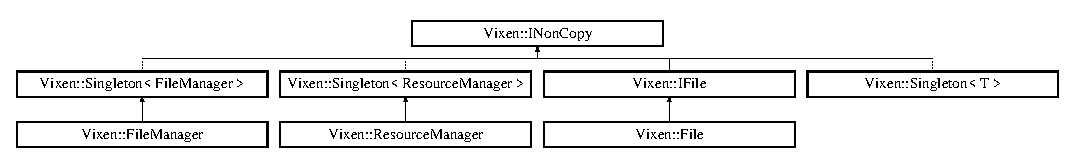
\includegraphics[height=1.757322cm]{classVixen_1_1INonCopy}
\end{center}
\end{figure}
\subsection*{Protected Member Functions}
\begin{DoxyCompactItemize}
\item 
\hyperlink{classVixen_1_1INonCopy_abee6536fcd39b24b4bc283402f9fd2c1}{I\+Non\+Copy} ()
\item 
\hyperlink{classVixen_1_1INonCopy_abfc5445a31c2102bd67b8b746d92a21b}{$\sim$\+I\+Non\+Copy} ()
\end{DoxyCompactItemize}


\subsection{Constructor \& Destructor Documentation}
\hypertarget{classVixen_1_1INonCopy_abee6536fcd39b24b4bc283402f9fd2c1}{}\index{Vixen\+::\+I\+Non\+Copy@{Vixen\+::\+I\+Non\+Copy}!I\+Non\+Copy@{I\+Non\+Copy}}
\index{I\+Non\+Copy@{I\+Non\+Copy}!Vixen\+::\+I\+Non\+Copy@{Vixen\+::\+I\+Non\+Copy}}
\subsubsection[{I\+Non\+Copy}]{\setlength{\rightskip}{0pt plus 5cm}Vixen\+::\+I\+Non\+Copy\+::\+I\+Non\+Copy (
\begin{DoxyParamCaption}
{}
\end{DoxyParamCaption}
)\hspace{0.3cm}{\ttfamily [inline]}, {\ttfamily [protected]}}\label{classVixen_1_1INonCopy_abee6536fcd39b24b4bc283402f9fd2c1}
\hypertarget{classVixen_1_1INonCopy_abfc5445a31c2102bd67b8b746d92a21b}{}\index{Vixen\+::\+I\+Non\+Copy@{Vixen\+::\+I\+Non\+Copy}!````~I\+Non\+Copy@{$\sim$\+I\+Non\+Copy}}
\index{````~I\+Non\+Copy@{$\sim$\+I\+Non\+Copy}!Vixen\+::\+I\+Non\+Copy@{Vixen\+::\+I\+Non\+Copy}}
\subsubsection[{$\sim$\+I\+Non\+Copy}]{\setlength{\rightskip}{0pt plus 5cm}Vixen\+::\+I\+Non\+Copy\+::$\sim$\+I\+Non\+Copy (
\begin{DoxyParamCaption}
{}
\end{DoxyParamCaption}
)\hspace{0.3cm}{\ttfamily [inline]}, {\ttfamily [protected]}}\label{classVixen_1_1INonCopy_abfc5445a31c2102bd67b8b746d92a21b}


The documentation for this class was generated from the following file\+:\begin{DoxyCompactItemize}
\item 
/home/debunez/\+Development/\+Vixen\+Engine/include/vcore/\hyperlink{vix__noncopy_8h}{vix\+\_\+noncopy.\+h}\end{DoxyCompactItemize}

\hypertarget{classVixen_1_1PathManager}{}\section{Vixen\+:\+:Path\+Manager Class Reference}
\label{classVixen_1_1PathManager}\index{Vixen\+::\+Path\+Manager@{Vixen\+::\+Path\+Manager}}


{\ttfamily \#include $<$vix\+\_\+pathmanager.\+h$>$}

\subsection*{Public Member Functions}
\begin{DoxyCompactItemize}
\item 
\hyperlink{classVixen_1_1PathManager_a36158e044f419f8ba5d72ceb848e6cc9}{Path\+Manager} ()
\end{DoxyCompactItemize}


\subsection{Constructor \& Destructor Documentation}
\hypertarget{classVixen_1_1PathManager_a36158e044f419f8ba5d72ceb848e6cc9}{}\index{Vixen\+::\+Path\+Manager@{Vixen\+::\+Path\+Manager}!Path\+Manager@{Path\+Manager}}
\index{Path\+Manager@{Path\+Manager}!Vixen\+::\+Path\+Manager@{Vixen\+::\+Path\+Manager}}
\subsubsection[{Path\+Manager}]{\setlength{\rightskip}{0pt plus 5cm}Vixen\+::\+Path\+Manager\+::\+Path\+Manager (
\begin{DoxyParamCaption}
{}
\end{DoxyParamCaption}
)}\label{classVixen_1_1PathManager_a36158e044f419f8ba5d72ceb848e6cc9}


The documentation for this class was generated from the following files\+:\begin{DoxyCompactItemize}
\item 
/home/debunez/\+Development/\+Vixen\+Engine/include/vcore/\hyperlink{vix__pathmanager_8h}{vix\+\_\+pathmanager.\+h}\item 
/home/debunez/\+Development/\+Vixen\+Engine/source/vcore/\hyperlink{vix__pathmanager_8cpp}{vix\+\_\+pathmanager.\+cpp}\end{DoxyCompactItemize}

\hypertarget{classVixen_1_1ResourceManager}{}\section{Vixen\+:\+:Resource\+Manager Class Reference}
\label{classVixen_1_1ResourceManager}\index{Vixen\+::\+Resource\+Manager@{Vixen\+::\+Resource\+Manager}}


{\ttfamily \#include $<$vix\+\_\+resourcemanager.\+h$>$}

Inheritance diagram for Vixen\+:\+:Resource\+Manager\+:\begin{figure}[H]
\begin{center}
\leavevmode
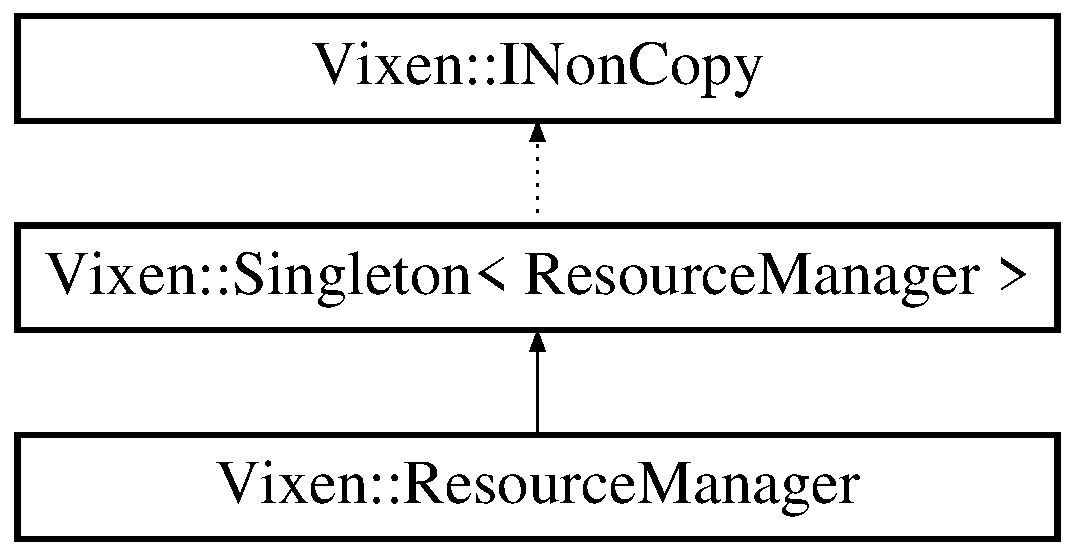
\includegraphics[height=3.000000cm]{classVixen_1_1ResourceManager}
\end{center}
\end{figure}
\subsection*{Public Member Functions}
\begin{DoxyCompactItemize}
\item 
\hyperlink{classVixen_1_1ResourceManager_a6b643c243582cdb8eab38e48cf6fa8cf}{$\sim$\+Resource\+Manager} ()
\end{DoxyCompactItemize}
\subsection*{Static Public Member Functions}
\begin{DoxyCompactItemize}
\item 
static void \hyperlink{classVixen_1_1ResourceManager_a3ca204897da35df704300c937e00c967}{Open\+Resource} (\hyperlink{vix__stringutil_8h_a561c282c415a5c38fd9a26325701e3bf}{U\+String} file\+Path)
\item 
static void \hyperlink{classVixen_1_1ResourceManager_a407b9c3d2700761287127de4d86b722e}{Open\+Resource} (\hyperlink{vix__stringutil_8h_a561c282c415a5c38fd9a26325701e3bf}{U\+String} file\+Name, \hyperlink{namespaceVixen_a0ddb8e6066715322f5a48e9b2beb2461}{Resource\+Type} type)
\end{DoxyCompactItemize}
\subsection*{Additional Inherited Members}


\subsection{Detailed Description}
\hyperlink{classVixen_1_1ResourceManager}{Resource\+Manager} class

Defines the resource manager object that is used to load game content into the \hyperlink{namespaceVixen}{Vixen} Game Engine at runtime. 

\subsection{Constructor \& Destructor Documentation}
\hypertarget{classVixen_1_1ResourceManager_a6b643c243582cdb8eab38e48cf6fa8cf}{}\index{Vixen\+::\+Resource\+Manager@{Vixen\+::\+Resource\+Manager}!````~Resource\+Manager@{$\sim$\+Resource\+Manager}}
\index{````~Resource\+Manager@{$\sim$\+Resource\+Manager}!Vixen\+::\+Resource\+Manager@{Vixen\+::\+Resource\+Manager}}
\subsubsection[{$\sim$\+Resource\+Manager}]{\setlength{\rightskip}{0pt plus 5cm}Vixen\+::\+Resource\+Manager\+::$\sim$\+Resource\+Manager (
\begin{DoxyParamCaption}
{}
\end{DoxyParamCaption}
)}\label{classVixen_1_1ResourceManager_a6b643c243582cdb8eab38e48cf6fa8cf}


\subsection{Member Function Documentation}
\hypertarget{classVixen_1_1ResourceManager_a3ca204897da35df704300c937e00c967}{}\index{Vixen\+::\+Resource\+Manager@{Vixen\+::\+Resource\+Manager}!Open\+Resource@{Open\+Resource}}
\index{Open\+Resource@{Open\+Resource}!Vixen\+::\+Resource\+Manager@{Vixen\+::\+Resource\+Manager}}
\subsubsection[{Open\+Resource}]{\setlength{\rightskip}{0pt plus 5cm}static void Vixen\+::\+Resource\+Manager\+::\+Open\+Resource (
\begin{DoxyParamCaption}
\item[{{\bf U\+String}}]{file\+Path}
\end{DoxyParamCaption}
)\hspace{0.3cm}{\ttfamily [static]}}\label{classVixen_1_1ResourceManager_a3ca204897da35df704300c937e00c967}
\hypertarget{classVixen_1_1ResourceManager_a407b9c3d2700761287127de4d86b722e}{}\index{Vixen\+::\+Resource\+Manager@{Vixen\+::\+Resource\+Manager}!Open\+Resource@{Open\+Resource}}
\index{Open\+Resource@{Open\+Resource}!Vixen\+::\+Resource\+Manager@{Vixen\+::\+Resource\+Manager}}
\subsubsection[{Open\+Resource}]{\setlength{\rightskip}{0pt plus 5cm}static void Vixen\+::\+Resource\+Manager\+::\+Open\+Resource (
\begin{DoxyParamCaption}
\item[{{\bf U\+String}}]{file\+Name, }
\item[{{\bf Resource\+Type}}]{type}
\end{DoxyParamCaption}
)\hspace{0.3cm}{\ttfamily [static]}}\label{classVixen_1_1ResourceManager_a407b9c3d2700761287127de4d86b722e}


The documentation for this class was generated from the following files\+:\begin{DoxyCompactItemize}
\item 
/home/debunez/\+Development/\+Vixen\+Engine/include/vcore/\hyperlink{vix__resourcemanager_8h}{vix\+\_\+resourcemanager.\+h}\item 
/home/debunez/\+Development/\+Vixen\+Engine/source/vcore/\hyperlink{vix__resourcemanager_8cpp}{vix\+\_\+resourcemanager.\+cpp}\end{DoxyCompactItemize}

\hypertarget{classVixen_1_1Singleton}{}\section{Vixen\+:\+:Singleton$<$ T $>$ Class Template Reference}
\label{classVixen_1_1Singleton}\index{Vixen\+::\+Singleton$<$ T $>$@{Vixen\+::\+Singleton$<$ T $>$}}


{\ttfamily \#include $<$vix\+\_\+singleton.\+h$>$}

Inheritance diagram for Vixen\+:\+:Singleton$<$ T $>$\+:\begin{figure}[H]
\begin{center}
\leavevmode
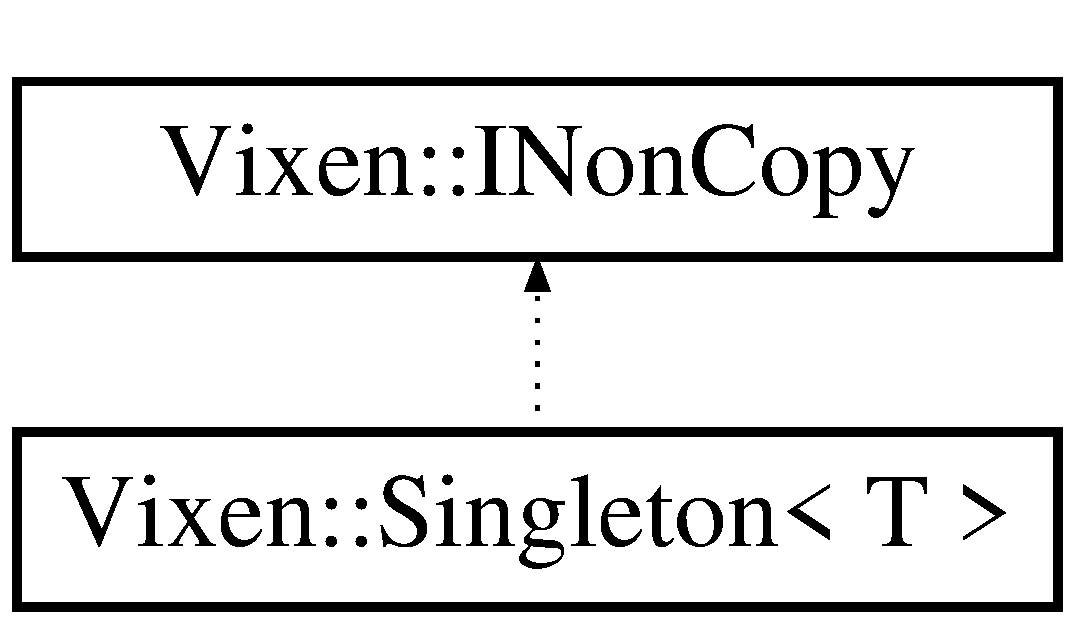
\includegraphics[height=2.000000cm]{classVixen_1_1Singleton}
\end{center}
\end{figure}
\subsection*{Static Public Member Functions}
\begin{DoxyCompactItemize}
\item 
static T \& \hyperlink{classVixen_1_1Singleton_a2b64eef896e902ce89a898432c0309fe}{instance} ()
\end{DoxyCompactItemize}
\subsection*{Protected Member Functions}
\begin{DoxyCompactItemize}
\item 
\hyperlink{classVixen_1_1Singleton_a741cc052dbc30e056d5513df31348841}{Singleton} ()
\end{DoxyCompactItemize}


\subsection{Constructor \& Destructor Documentation}
\hypertarget{classVixen_1_1Singleton_a741cc052dbc30e056d5513df31348841}{}\index{Vixen\+::\+Singleton@{Vixen\+::\+Singleton}!Singleton@{Singleton}}
\index{Singleton@{Singleton}!Vixen\+::\+Singleton@{Vixen\+::\+Singleton}}
\subsubsection[{Singleton}]{\setlength{\rightskip}{0pt plus 5cm}template$<$typename T$>$ {\bf Vixen\+::\+Singleton}$<$ T $>$\+::{\bf Singleton} (
\begin{DoxyParamCaption}
{}
\end{DoxyParamCaption}
)\hspace{0.3cm}{\ttfamily [inline]}, {\ttfamily [explicit]}, {\ttfamily [protected]}}\label{classVixen_1_1Singleton_a741cc052dbc30e056d5513df31348841}


\subsection{Member Function Documentation}
\hypertarget{classVixen_1_1Singleton_a2b64eef896e902ce89a898432c0309fe}{}\index{Vixen\+::\+Singleton@{Vixen\+::\+Singleton}!instance@{instance}}
\index{instance@{instance}!Vixen\+::\+Singleton@{Vixen\+::\+Singleton}}
\subsubsection[{instance}]{\setlength{\rightskip}{0pt plus 5cm}template$<$typename T$>$ static T\& {\bf Vixen\+::\+Singleton}$<$ T $>$\+::instance (
\begin{DoxyParamCaption}
{}
\end{DoxyParamCaption}
)\hspace{0.3cm}{\ttfamily [inline]}, {\ttfamily [static]}}\label{classVixen_1_1Singleton_a2b64eef896e902ce89a898432c0309fe}


The documentation for this class was generated from the following file\+:\begin{DoxyCompactItemize}
\item 
/home/debunez/\+Development/\+Vixen\+Engine/include/vcore/\hyperlink{vix__singleton_8h}{vix\+\_\+singleton.\+h}\end{DoxyCompactItemize}

\chapter{File Documentation}
\hypertarget{vix__algorithms_8h}{}\section{/home/debunez/\+Development/\+Vixen\+Engine/include/vcore/vix\+\_\+algorithms.h File Reference}
\label{vix__algorithms_8h}\index{/home/debunez/\+Development/\+Vixen\+Engine/include/vcore/vix\+\_\+algorithms.\+h@{/home/debunez/\+Development/\+Vixen\+Engine/include/vcore/vix\+\_\+algorithms.\+h}}
{\ttfamily \#include $<$vix\+\_\+platform.\+h$>$}\\*
{\ttfamily \#include $<$algorithm$>$}\\*
{\ttfamily \#include $<$vector$>$}\\*
\subsection*{Namespaces}
\begin{DoxyCompactItemize}
\item 
 \hyperlink{namespaceVixen}{Vixen}
\end{DoxyCompactItemize}

\hypertarget{vix__containers_8h}{}\section{/home/debunez/\+Development/\+Vixen\+Engine/include/vcore/vix\+\_\+containers.h File Reference}
\label{vix__containers_8h}\index{/home/debunez/\+Development/\+Vixen\+Engine/include/vcore/vix\+\_\+containers.\+h@{/home/debunez/\+Development/\+Vixen\+Engine/include/vcore/vix\+\_\+containers.\+h}}
{\ttfamily \#include $<$vix\+\_\+platform.\+h$>$}\\*
{\ttfamily \#include $<$list$>$}\\*
{\ttfamily \#include $<$vector$>$}\\*

\hypertarget{vix__content_8h}{}\section{/home/debunez/\+Development/\+Vixen\+Engine/include/vcore/vix\+\_\+content.h File Reference}
\label{vix__content_8h}\index{/home/debunez/\+Development/\+Vixen\+Engine/include/vcore/vix\+\_\+content.\+h@{/home/debunez/\+Development/\+Vixen\+Engine/include/vcore/vix\+\_\+content.\+h}}
{\ttfamily \#include $<$vix\+\_\+platform.\+h$>$}\\*
\subsection*{Classes}
\begin{DoxyCompactItemize}
\item 
class \hyperlink{classVixen_1_1IContent}{Vixen\+::\+I\+Content}
\end{DoxyCompactItemize}
\subsection*{Namespaces}
\begin{DoxyCompactItemize}
\item 
 \hyperlink{namespaceVixen}{Vixen}
\end{DoxyCompactItemize}

\hypertarget{vix__debugutil_8h}{}\section{/home/debunez/\+Development/\+Vixen\+Engine/include/vcore/vix\+\_\+debugutil.h File Reference}
\label{vix__debugutil_8h}\index{/home/debunez/\+Development/\+Vixen\+Engine/include/vcore/vix\+\_\+debugutil.\+h@{/home/debunez/\+Development/\+Vixen\+Engine/include/vcore/vix\+\_\+debugutil.\+h}}
{\ttfamily \#include $<$vix\+\_\+platform.\+h$>$}\\*
{\ttfamily \#include $<$vix\+\_\+stringutil.\+h$>$}\\*
{\ttfamily \#include $<$iostream$>$}\\*
{\ttfamily \#include $<$iomanip$>$}\\*
{\ttfamily \#include $<$chrono$>$}\\*
{\ttfamily \#include $<$ctime$>$}\\*
\subsection*{Namespaces}
\begin{DoxyCompactItemize}
\item 
 \hyperlink{namespaceVixen}{Vixen}
\end{DoxyCompactItemize}
\subsection*{Macros}
\begin{DoxyCompactItemize}
\item 
\#define \hyperlink{vix__debugutil_8h_a6adf8f63b8ae346e5e34f2751d69cfc2}{V\+I\+X\+\_\+\+S\+T\+R\+I\+N\+G\+I\+F\+Y}(x)~\#x
\item 
\#define \hyperlink{vix__debugutil_8h_aacc867af2d286992bab0799c8f17e650}{V\+I\+X\+\_\+\+S\+F\+Y\+\_\+}(x)~\hyperlink{vix__debugutil_8h_a6adf8f63b8ae346e5e34f2751d69cfc2}{V\+I\+X\+\_\+\+S\+T\+R\+I\+N\+G\+I\+F\+Y}(x)
\item 
\#define \hyperlink{vix__debugutil_8h_a9296dc502535b7e7b60cbdf7741b93be}{V\+I\+X\+\_\+\+S\+F\+Y\+\_\+\+F\+U\+N\+C}~\hyperlink{vix__debugutil_8h_aacc867af2d286992bab0799c8f17e650}{V\+I\+X\+\_\+\+S\+F\+Y\+\_\+}(\+\_\+\+\_\+\+F\+U\+N\+C\+T\+I\+O\+N\+\_\+\+\_\+)
\item 
\#define \hyperlink{vix__debugutil_8h_a03dd4429956c4e407ada527f93964231}{V\+I\+X\+\_\+\+S\+F\+Y\+\_\+\+L\+I\+N\+E}~\hyperlink{vix__debugutil_8h_aacc867af2d286992bab0799c8f17e650}{V\+I\+X\+\_\+\+S\+F\+Y\+\_\+}(\+\_\+\+\_\+\+L\+I\+N\+E\+\_\+\+\_\+)
\item 
\#define \hyperlink{vix__debugutil_8h_a9a88d5011ad9b0b557d7fc2ae67dcf55}{V\+I\+X\+\_\+\+S\+F\+Y\+\_\+\+F\+I\+L\+E}~\hyperlink{vix__debugutil_8h_aacc867af2d286992bab0799c8f17e650}{V\+I\+X\+\_\+\+S\+F\+Y\+\_\+}(\+\_\+\+\_\+\+F\+I\+L\+E\+\_\+\+\_\+)
\item 
\#define \hyperlink{vix__debugutil_8h_a596d7e6d8219096a401f24f38fd296d9}{V\+I\+X\+\_\+\+L\+O\+G\+\_\+\+F\+I\+L\+E}~\char`\"{}F\+I\+L\+E\+: \char`\"{} V\+I\+X\+\_\+\+S\+F\+Y\+\_\+\+F\+I\+L\+E
\item 
\#define \hyperlink{vix__debugutil_8h_ade8ee4152ed032060a05c6a2af1d89e0}{V\+I\+X\+\_\+\+L\+O\+G\+\_\+\+L\+I\+N\+E}~\char`\"{}L\+I\+N\+E\+: \char`\"{} V\+I\+X\+\_\+\+S\+F\+Y\+\_\+\+L\+I\+N\+E
\item 
\#define \hyperlink{vix__debugutil_8h_a219aa98d61c77b1b0f30dea10b26fded}{V\+I\+X\+\_\+\+L\+O\+G\+\_\+\+F\+U\+N\+C}~\char`\"{}F\+U\+N\+C\+: \char`\"{} \+\_\+\+\_\+\+F\+U\+N\+C\+T\+I\+O\+N\+\_\+\+\_\+
\item 
\#define \hyperlink{vix__debugutil_8h_a6a7844902f0adc1d465e50a4c9cd54b7}{V\+I\+X\+\_\+\+L\+O\+G\+\_\+\+P\+R\+E\+F\+I\+X}~\hyperlink{vix__debugutil_8h_a596d7e6d8219096a401f24f38fd296d9}{V\+I\+X\+\_\+\+L\+O\+G\+\_\+\+F\+I\+L\+E} \char`\"{}\textbackslash{}n\char`\"{} V\+I\+X\+\_\+\+L\+O\+G\+\_\+\+F\+U\+N\+C \char`\"{}\textbackslash{}n\char`\"{} V\+I\+X\+\_\+\+L\+O\+G\+\_\+\+L\+I\+N\+E \char`\"{}\textbackslash{}n\char`\"{}
\end{DoxyCompactItemize}
\subsection*{Functions}
\begin{DoxyCompactItemize}
\item 
void \hyperlink{namespaceVixen_ae5d8286e89335780589abef43cffe82b}{Vixen\+::\+Console\+Write\+Err} (const \hyperlink{vix__stringutil_8h_a561c282c415a5c38fd9a26325701e3bf}{U\+String} \&text)
\item 
int \hyperlink{namespaceVixen_a98ec16e2cd362c7bc44690a5197c6c1e}{Vixen\+::\+V\+Debug\+Print\+F} (const \hyperlink{vix__stringutil_8h_adc2ae6d46e5cd3718f5446c8d2a2c5ac}{U\+Char} $\ast$format, va\+\_\+list arg\+List)
\item 
int \hyperlink{namespaceVixen_acedf76acc71be060abeab28f299d1314}{Vixen\+::\+Debug\+Print\+F} (const \hyperlink{vix__stringutil_8h_adc2ae6d46e5cd3718f5446c8d2a2c5ac}{U\+Char} $\ast$format,...)
\item 
\hyperlink{vix__platform_8h_afdaa33aa7411dace34f16eb161ffaf35}{V\+I\+X\+\_\+\+A\+P\+I} \hyperlink{vix__stringutil_8h_a561c282c415a5c38fd9a26325701e3bf}{U\+String} \hyperlink{namespaceVixen_a2ad0f14ebc1c95e994a11867d2daf6cf}{Vixen\+::\+Debug\+Time\+Stamp} ()
\end{DoxyCompactItemize}


\subsection{Macro Definition Documentation}
\hypertarget{vix__debugutil_8h_a596d7e6d8219096a401f24f38fd296d9}{}\index{vix\+\_\+debugutil.\+h@{vix\+\_\+debugutil.\+h}!V\+I\+X\+\_\+\+L\+O\+G\+\_\+\+F\+I\+L\+E@{V\+I\+X\+\_\+\+L\+O\+G\+\_\+\+F\+I\+L\+E}}
\index{V\+I\+X\+\_\+\+L\+O\+G\+\_\+\+F\+I\+L\+E@{V\+I\+X\+\_\+\+L\+O\+G\+\_\+\+F\+I\+L\+E}!vix\+\_\+debugutil.\+h@{vix\+\_\+debugutil.\+h}}
\subsubsection[{V\+I\+X\+\_\+\+L\+O\+G\+\_\+\+F\+I\+L\+E}]{\setlength{\rightskip}{0pt plus 5cm}\#define V\+I\+X\+\_\+\+L\+O\+G\+\_\+\+F\+I\+L\+E~\char`\"{}F\+I\+L\+E\+: \char`\"{} V\+I\+X\+\_\+\+S\+F\+Y\+\_\+\+F\+I\+L\+E}\label{vix__debugutil_8h_a596d7e6d8219096a401f24f38fd296d9}
\hypertarget{vix__debugutil_8h_a219aa98d61c77b1b0f30dea10b26fded}{}\index{vix\+\_\+debugutil.\+h@{vix\+\_\+debugutil.\+h}!V\+I\+X\+\_\+\+L\+O\+G\+\_\+\+F\+U\+N\+C@{V\+I\+X\+\_\+\+L\+O\+G\+\_\+\+F\+U\+N\+C}}
\index{V\+I\+X\+\_\+\+L\+O\+G\+\_\+\+F\+U\+N\+C@{V\+I\+X\+\_\+\+L\+O\+G\+\_\+\+F\+U\+N\+C}!vix\+\_\+debugutil.\+h@{vix\+\_\+debugutil.\+h}}
\subsubsection[{V\+I\+X\+\_\+\+L\+O\+G\+\_\+\+F\+U\+N\+C}]{\setlength{\rightskip}{0pt plus 5cm}\#define V\+I\+X\+\_\+\+L\+O\+G\+\_\+\+F\+U\+N\+C~\char`\"{}F\+U\+N\+C\+: \char`\"{} \+\_\+\+\_\+\+F\+U\+N\+C\+T\+I\+O\+N\+\_\+\+\_\+}\label{vix__debugutil_8h_a219aa98d61c77b1b0f30dea10b26fded}
\hypertarget{vix__debugutil_8h_ade8ee4152ed032060a05c6a2af1d89e0}{}\index{vix\+\_\+debugutil.\+h@{vix\+\_\+debugutil.\+h}!V\+I\+X\+\_\+\+L\+O\+G\+\_\+\+L\+I\+N\+E@{V\+I\+X\+\_\+\+L\+O\+G\+\_\+\+L\+I\+N\+E}}
\index{V\+I\+X\+\_\+\+L\+O\+G\+\_\+\+L\+I\+N\+E@{V\+I\+X\+\_\+\+L\+O\+G\+\_\+\+L\+I\+N\+E}!vix\+\_\+debugutil.\+h@{vix\+\_\+debugutil.\+h}}
\subsubsection[{V\+I\+X\+\_\+\+L\+O\+G\+\_\+\+L\+I\+N\+E}]{\setlength{\rightskip}{0pt plus 5cm}\#define V\+I\+X\+\_\+\+L\+O\+G\+\_\+\+L\+I\+N\+E~\char`\"{}L\+I\+N\+E\+: \char`\"{} V\+I\+X\+\_\+\+S\+F\+Y\+\_\+\+L\+I\+N\+E}\label{vix__debugutil_8h_ade8ee4152ed032060a05c6a2af1d89e0}
\hypertarget{vix__debugutil_8h_a6a7844902f0adc1d465e50a4c9cd54b7}{}\index{vix\+\_\+debugutil.\+h@{vix\+\_\+debugutil.\+h}!V\+I\+X\+\_\+\+L\+O\+G\+\_\+\+P\+R\+E\+F\+I\+X@{V\+I\+X\+\_\+\+L\+O\+G\+\_\+\+P\+R\+E\+F\+I\+X}}
\index{V\+I\+X\+\_\+\+L\+O\+G\+\_\+\+P\+R\+E\+F\+I\+X@{V\+I\+X\+\_\+\+L\+O\+G\+\_\+\+P\+R\+E\+F\+I\+X}!vix\+\_\+debugutil.\+h@{vix\+\_\+debugutil.\+h}}
\subsubsection[{V\+I\+X\+\_\+\+L\+O\+G\+\_\+\+P\+R\+E\+F\+I\+X}]{\setlength{\rightskip}{0pt plus 5cm}\#define V\+I\+X\+\_\+\+L\+O\+G\+\_\+\+P\+R\+E\+F\+I\+X~{\bf V\+I\+X\+\_\+\+L\+O\+G\+\_\+\+F\+I\+L\+E} \char`\"{}\textbackslash{}n\char`\"{} V\+I\+X\+\_\+\+L\+O\+G\+\_\+\+F\+U\+N\+C \char`\"{}\textbackslash{}n\char`\"{} V\+I\+X\+\_\+\+L\+O\+G\+\_\+\+L\+I\+N\+E \char`\"{}\textbackslash{}n\char`\"{}}\label{vix__debugutil_8h_a6a7844902f0adc1d465e50a4c9cd54b7}
\hypertarget{vix__debugutil_8h_aacc867af2d286992bab0799c8f17e650}{}\index{vix\+\_\+debugutil.\+h@{vix\+\_\+debugutil.\+h}!V\+I\+X\+\_\+\+S\+F\+Y\+\_\+@{V\+I\+X\+\_\+\+S\+F\+Y\+\_\+}}
\index{V\+I\+X\+\_\+\+S\+F\+Y\+\_\+@{V\+I\+X\+\_\+\+S\+F\+Y\+\_\+}!vix\+\_\+debugutil.\+h@{vix\+\_\+debugutil.\+h}}
\subsubsection[{V\+I\+X\+\_\+\+S\+F\+Y\+\_\+}]{\setlength{\rightskip}{0pt plus 5cm}\#define V\+I\+X\+\_\+\+S\+F\+Y\+\_\+(
\begin{DoxyParamCaption}
\item[{}]{x}
\end{DoxyParamCaption}
)~{\bf V\+I\+X\+\_\+\+S\+T\+R\+I\+N\+G\+I\+F\+Y}(x)}\label{vix__debugutil_8h_aacc867af2d286992bab0799c8f17e650}
\hypertarget{vix__debugutil_8h_a9a88d5011ad9b0b557d7fc2ae67dcf55}{}\index{vix\+\_\+debugutil.\+h@{vix\+\_\+debugutil.\+h}!V\+I\+X\+\_\+\+S\+F\+Y\+\_\+\+F\+I\+L\+E@{V\+I\+X\+\_\+\+S\+F\+Y\+\_\+\+F\+I\+L\+E}}
\index{V\+I\+X\+\_\+\+S\+F\+Y\+\_\+\+F\+I\+L\+E@{V\+I\+X\+\_\+\+S\+F\+Y\+\_\+\+F\+I\+L\+E}!vix\+\_\+debugutil.\+h@{vix\+\_\+debugutil.\+h}}
\subsubsection[{V\+I\+X\+\_\+\+S\+F\+Y\+\_\+\+F\+I\+L\+E}]{\setlength{\rightskip}{0pt plus 5cm}\#define V\+I\+X\+\_\+\+S\+F\+Y\+\_\+\+F\+I\+L\+E~{\bf V\+I\+X\+\_\+\+S\+F\+Y\+\_\+}(\+\_\+\+\_\+\+F\+I\+L\+E\+\_\+\+\_\+)}\label{vix__debugutil_8h_a9a88d5011ad9b0b557d7fc2ae67dcf55}
\hypertarget{vix__debugutil_8h_a9296dc502535b7e7b60cbdf7741b93be}{}\index{vix\+\_\+debugutil.\+h@{vix\+\_\+debugutil.\+h}!V\+I\+X\+\_\+\+S\+F\+Y\+\_\+\+F\+U\+N\+C@{V\+I\+X\+\_\+\+S\+F\+Y\+\_\+\+F\+U\+N\+C}}
\index{V\+I\+X\+\_\+\+S\+F\+Y\+\_\+\+F\+U\+N\+C@{V\+I\+X\+\_\+\+S\+F\+Y\+\_\+\+F\+U\+N\+C}!vix\+\_\+debugutil.\+h@{vix\+\_\+debugutil.\+h}}
\subsubsection[{V\+I\+X\+\_\+\+S\+F\+Y\+\_\+\+F\+U\+N\+C}]{\setlength{\rightskip}{0pt plus 5cm}\#define V\+I\+X\+\_\+\+S\+F\+Y\+\_\+\+F\+U\+N\+C~{\bf V\+I\+X\+\_\+\+S\+F\+Y\+\_\+}(\+\_\+\+\_\+\+F\+U\+N\+C\+T\+I\+O\+N\+\_\+\+\_\+)}\label{vix__debugutil_8h_a9296dc502535b7e7b60cbdf7741b93be}
\hypertarget{vix__debugutil_8h_a03dd4429956c4e407ada527f93964231}{}\index{vix\+\_\+debugutil.\+h@{vix\+\_\+debugutil.\+h}!V\+I\+X\+\_\+\+S\+F\+Y\+\_\+\+L\+I\+N\+E@{V\+I\+X\+\_\+\+S\+F\+Y\+\_\+\+L\+I\+N\+E}}
\index{V\+I\+X\+\_\+\+S\+F\+Y\+\_\+\+L\+I\+N\+E@{V\+I\+X\+\_\+\+S\+F\+Y\+\_\+\+L\+I\+N\+E}!vix\+\_\+debugutil.\+h@{vix\+\_\+debugutil.\+h}}
\subsubsection[{V\+I\+X\+\_\+\+S\+F\+Y\+\_\+\+L\+I\+N\+E}]{\setlength{\rightskip}{0pt plus 5cm}\#define V\+I\+X\+\_\+\+S\+F\+Y\+\_\+\+L\+I\+N\+E~{\bf V\+I\+X\+\_\+\+S\+F\+Y\+\_\+}(\+\_\+\+\_\+\+L\+I\+N\+E\+\_\+\+\_\+)}\label{vix__debugutil_8h_a03dd4429956c4e407ada527f93964231}
\hypertarget{vix__debugutil_8h_a6adf8f63b8ae346e5e34f2751d69cfc2}{}\index{vix\+\_\+debugutil.\+h@{vix\+\_\+debugutil.\+h}!V\+I\+X\+\_\+\+S\+T\+R\+I\+N\+G\+I\+F\+Y@{V\+I\+X\+\_\+\+S\+T\+R\+I\+N\+G\+I\+F\+Y}}
\index{V\+I\+X\+\_\+\+S\+T\+R\+I\+N\+G\+I\+F\+Y@{V\+I\+X\+\_\+\+S\+T\+R\+I\+N\+G\+I\+F\+Y}!vix\+\_\+debugutil.\+h@{vix\+\_\+debugutil.\+h}}
\subsubsection[{V\+I\+X\+\_\+\+S\+T\+R\+I\+N\+G\+I\+F\+Y}]{\setlength{\rightskip}{0pt plus 5cm}\#define V\+I\+X\+\_\+\+S\+T\+R\+I\+N\+G\+I\+F\+Y(
\begin{DoxyParamCaption}
\item[{}]{x}
\end{DoxyParamCaption}
)~\#x}\label{vix__debugutil_8h_a6adf8f63b8ae346e5e34f2751d69cfc2}

\hypertarget{vix__enumutil_8h}{}\section{/home/debunez/\+Development/\+Vixen\+Engine/include/vcore/vix\+\_\+enumutil.h File Reference}
\label{vix__enumutil_8h}\index{/home/debunez/\+Development/\+Vixen\+Engine/include/vcore/vix\+\_\+enumutil.\+h@{/home/debunez/\+Development/\+Vixen\+Engine/include/vcore/vix\+\_\+enumutil.\+h}}
{\ttfamily \#include $<$vix\+\_\+platform.\+h$>$}\\*
{\ttfamily \#include $<$vix\+\_\+stringutil.\+h$>$}\\*
\subsection*{Classes}
\begin{DoxyCompactItemize}
\item 
class \hyperlink{classEnumStrings}{Enum\+Strings$<$ T $>$}
\end{DoxyCompactItemize}
\subsection*{Functions}
\begin{DoxyCompactItemize}
\item 
{\footnotesize template$<$typename T $>$ }\\const std\+::string \hyperlink{vix__enumutil_8h_ab4d5bcdc3bd778adba7fc5c96c7eb583}{Enum\+String} (T \+\_\+enum)
\end{DoxyCompactItemize}


\subsection{Function Documentation}
\hypertarget{vix__enumutil_8h_ab4d5bcdc3bd778adba7fc5c96c7eb583}{}\index{vix\+\_\+enumutil.\+h@{vix\+\_\+enumutil.\+h}!Enum\+String@{Enum\+String}}
\index{Enum\+String@{Enum\+String}!vix\+\_\+enumutil.\+h@{vix\+\_\+enumutil.\+h}}
\subsubsection[{Enum\+String}]{\setlength{\rightskip}{0pt plus 5cm}template$<$typename T $>$ const std\+::string Enum\+String (
\begin{DoxyParamCaption}
\item[{T}]{\+\_\+enum}
\end{DoxyParamCaption}
)}\label{vix__enumutil_8h_ab4d5bcdc3bd778adba7fc5c96c7eb583}

\hypertarget{vix__errglobals_8h}{}\section{/home/debunez/\+Development/\+Vixen\+Engine/include/vcore/vix\+\_\+errglobals.h File Reference}
\label{vix__errglobals_8h}\index{/home/debunez/\+Development/\+Vixen\+Engine/include/vcore/vix\+\_\+errglobals.\+h@{/home/debunez/\+Development/\+Vixen\+Engine/include/vcore/vix\+\_\+errglobals.\+h}}
{\ttfamily \#include $<$vix\+\_\+platform.\+h$>$}\\*
{\ttfamily \#include $<$vix\+\_\+stringutil.\+h$>$}\\*
\subsection*{Enumerations}
\begin{DoxyCompactItemize}
\item 
enum \hyperlink{vix__errglobals_8h_a072137da885565f4c2f9e9116485659a}{Err\+Code} \{ \\*
\hyperlink{vix__errglobals_8h_a072137da885565f4c2f9e9116485659aa3e52caccdab7c168a1b5cfc7f0221c3b}{Err\+Code\+::\+E\+R\+R\+\_\+\+F\+A\+I\+L\+U\+R\+E}, 
\hyperlink{vix__errglobals_8h_a072137da885565f4c2f9e9116485659aa5fcef47c9a169f2e1e974fbd8ed06e40}{Err\+Code\+::\+E\+R\+R\+\_\+\+S\+U\+C\+C\+E\+S\+S}, 
\hyperlink{vix__errglobals_8h_a072137da885565f4c2f9e9116485659aae6376aeec2fcbe009fd272d5d1376d2c}{Err\+Code\+::\+E\+R\+R\+\_\+\+N\+U\+L\+L\+\_\+\+P\+A\+T\+H}, 
\hyperlink{vix__errglobals_8h_a072137da885565f4c2f9e9116485659aa374d85c1056381de8d46c382681fafd9}{Err\+Code\+::\+E\+R\+R\+\_\+\+F\+I\+L\+E\+\_\+\+N\+O\+T\+\_\+\+F\+O\+U\+N\+D}, 
\\*
\hyperlink{vix__errglobals_8h_a072137da885565f4c2f9e9116485659aa72c3f5615c349cc54720041476fa0277}{Err\+Code\+::\+E\+R\+R\+\_\+\+S\+D\+L\+\_\+\+I\+N\+I\+T\+\_\+\+F\+A\+I\+L}, 
\hyperlink{vix__errglobals_8h_a072137da885565f4c2f9e9116485659aad8a86dc6403864e72ed50db5bbca5fc8}{Err\+Code\+::\+E\+R\+R\+\_\+\+S\+D\+L\+\_\+\+C\+R\+E\+A\+T\+E\+\_\+\+F\+A\+I\+L}, 
\hyperlink{vix__errglobals_8h_a072137da885565f4c2f9e9116485659aa5f4c587130b097cfa2d6da80de8e698b}{Err\+Code\+::\+E\+R\+R\+\_\+\+I\+M\+A\+G\+E\+\_\+\+L\+O\+A\+D\+\_\+\+F\+A\+I\+L}, 
\hyperlink{vix__errglobals_8h_a072137da885565f4c2f9e9116485659aa7690dbbc8072b8b6070677dfe0da841e}{Err\+Code\+::\+E\+R\+R\+\_\+\+X\+M\+L\+\_\+\+R\+E\+A\+D\+\_\+\+F\+A\+I\+L}, 
\\*
\hyperlink{vix__errglobals_8h_a072137da885565f4c2f9e9116485659aa4e25209ceef6b55b9ddc344412427336}{Err\+Code\+::\+E\+R\+R\+\_\+\+X\+M\+L\+\_\+\+W\+R\+I\+T\+E\+\_\+\+F\+A\+I\+L}, 
\hyperlink{vix__errglobals_8h_a072137da885565f4c2f9e9116485659aa8139a37c0a0f1efa35a46ba4e8a92a2e}{Err\+Code\+::\+E\+R\+R\+\_\+\+G\+L\+E\+W\+\_\+\+I\+N\+I\+T\+\_\+\+F\+A\+I\+L}
 \}
\end{DoxyCompactItemize}
\subsection*{Functions}
\begin{DoxyCompactItemize}
\item 
\hyperlink{vix__stringutil_8h_a561c282c415a5c38fd9a26325701e3bf}{U\+String} \hyperlink{vix__errglobals_8h_a94dcf104f9daba9b228df2be46507d29}{Err\+Code\+String} (\hyperlink{vix__errglobals_8h_a072137da885565f4c2f9e9116485659a}{Err\+Code} error)
\item 
bool \hyperlink{vix__errglobals_8h_a03486e2efafef6911389c4e76a25492f}{Check\+Error} (\hyperlink{vix__errglobals_8h_a072137da885565f4c2f9e9116485659a}{Err\+Code} error)
\end{DoxyCompactItemize}


\subsection{Enumeration Type Documentation}
\hypertarget{vix__errglobals_8h_a072137da885565f4c2f9e9116485659a}{}\index{vix\+\_\+errglobals.\+h@{vix\+\_\+errglobals.\+h}!Err\+Code@{Err\+Code}}
\index{Err\+Code@{Err\+Code}!vix\+\_\+errglobals.\+h@{vix\+\_\+errglobals.\+h}}
\subsubsection[{Err\+Code}]{\setlength{\rightskip}{0pt plus 5cm}enum {\bf Err\+Code}\hspace{0.3cm}{\ttfamily [strong]}}\label{vix__errglobals_8h_a072137da885565f4c2f9e9116485659a}
\begin{Desc}
\item[Enumerator]\par
\begin{description}
\index{E\+R\+R\+\_\+\+F\+A\+I\+L\+U\+R\+E@{E\+R\+R\+\_\+\+F\+A\+I\+L\+U\+R\+E}!vix\+\_\+errglobals.\+h@{vix\+\_\+errglobals.\+h}}\index{vix\+\_\+errglobals.\+h@{vix\+\_\+errglobals.\+h}!E\+R\+R\+\_\+\+F\+A\+I\+L\+U\+R\+E@{E\+R\+R\+\_\+\+F\+A\+I\+L\+U\+R\+E}}\item[{\em 
\hypertarget{vix__errglobals_8h_a072137da885565f4c2f9e9116485659aa3e52caccdab7c168a1b5cfc7f0221c3b}{}E\+R\+R\+\_\+\+F\+A\+I\+L\+U\+R\+E\label{vix__errglobals_8h_a072137da885565f4c2f9e9116485659aa3e52caccdab7c168a1b5cfc7f0221c3b}
}]\index{E\+R\+R\+\_\+\+S\+U\+C\+C\+E\+S\+S@{E\+R\+R\+\_\+\+S\+U\+C\+C\+E\+S\+S}!vix\+\_\+errglobals.\+h@{vix\+\_\+errglobals.\+h}}\index{vix\+\_\+errglobals.\+h@{vix\+\_\+errglobals.\+h}!E\+R\+R\+\_\+\+S\+U\+C\+C\+E\+S\+S@{E\+R\+R\+\_\+\+S\+U\+C\+C\+E\+S\+S}}\item[{\em 
\hypertarget{vix__errglobals_8h_a072137da885565f4c2f9e9116485659aa5fcef47c9a169f2e1e974fbd8ed06e40}{}E\+R\+R\+\_\+\+S\+U\+C\+C\+E\+S\+S\label{vix__errglobals_8h_a072137da885565f4c2f9e9116485659aa5fcef47c9a169f2e1e974fbd8ed06e40}
}]\index{E\+R\+R\+\_\+\+N\+U\+L\+L\+\_\+\+P\+A\+T\+H@{E\+R\+R\+\_\+\+N\+U\+L\+L\+\_\+\+P\+A\+T\+H}!vix\+\_\+errglobals.\+h@{vix\+\_\+errglobals.\+h}}\index{vix\+\_\+errglobals.\+h@{vix\+\_\+errglobals.\+h}!E\+R\+R\+\_\+\+N\+U\+L\+L\+\_\+\+P\+A\+T\+H@{E\+R\+R\+\_\+\+N\+U\+L\+L\+\_\+\+P\+A\+T\+H}}\item[{\em 
\hypertarget{vix__errglobals_8h_a072137da885565f4c2f9e9116485659aae6376aeec2fcbe009fd272d5d1376d2c}{}E\+R\+R\+\_\+\+N\+U\+L\+L\+\_\+\+P\+A\+T\+H\label{vix__errglobals_8h_a072137da885565f4c2f9e9116485659aae6376aeec2fcbe009fd272d5d1376d2c}
}]\index{E\+R\+R\+\_\+\+F\+I\+L\+E\+\_\+\+N\+O\+T\+\_\+\+F\+O\+U\+N\+D@{E\+R\+R\+\_\+\+F\+I\+L\+E\+\_\+\+N\+O\+T\+\_\+\+F\+O\+U\+N\+D}!vix\+\_\+errglobals.\+h@{vix\+\_\+errglobals.\+h}}\index{vix\+\_\+errglobals.\+h@{vix\+\_\+errglobals.\+h}!E\+R\+R\+\_\+\+F\+I\+L\+E\+\_\+\+N\+O\+T\+\_\+\+F\+O\+U\+N\+D@{E\+R\+R\+\_\+\+F\+I\+L\+E\+\_\+\+N\+O\+T\+\_\+\+F\+O\+U\+N\+D}}\item[{\em 
\hypertarget{vix__errglobals_8h_a072137da885565f4c2f9e9116485659aa374d85c1056381de8d46c382681fafd9}{}E\+R\+R\+\_\+\+F\+I\+L\+E\+\_\+\+N\+O\+T\+\_\+\+F\+O\+U\+N\+D\label{vix__errglobals_8h_a072137da885565f4c2f9e9116485659aa374d85c1056381de8d46c382681fafd9}
}]\index{E\+R\+R\+\_\+\+S\+D\+L\+\_\+\+I\+N\+I\+T\+\_\+\+F\+A\+I\+L@{E\+R\+R\+\_\+\+S\+D\+L\+\_\+\+I\+N\+I\+T\+\_\+\+F\+A\+I\+L}!vix\+\_\+errglobals.\+h@{vix\+\_\+errglobals.\+h}}\index{vix\+\_\+errglobals.\+h@{vix\+\_\+errglobals.\+h}!E\+R\+R\+\_\+\+S\+D\+L\+\_\+\+I\+N\+I\+T\+\_\+\+F\+A\+I\+L@{E\+R\+R\+\_\+\+S\+D\+L\+\_\+\+I\+N\+I\+T\+\_\+\+F\+A\+I\+L}}\item[{\em 
\hypertarget{vix__errglobals_8h_a072137da885565f4c2f9e9116485659aa72c3f5615c349cc54720041476fa0277}{}E\+R\+R\+\_\+\+S\+D\+L\+\_\+\+I\+N\+I\+T\+\_\+\+F\+A\+I\+L\label{vix__errglobals_8h_a072137da885565f4c2f9e9116485659aa72c3f5615c349cc54720041476fa0277}
}]\index{E\+R\+R\+\_\+\+S\+D\+L\+\_\+\+C\+R\+E\+A\+T\+E\+\_\+\+F\+A\+I\+L@{E\+R\+R\+\_\+\+S\+D\+L\+\_\+\+C\+R\+E\+A\+T\+E\+\_\+\+F\+A\+I\+L}!vix\+\_\+errglobals.\+h@{vix\+\_\+errglobals.\+h}}\index{vix\+\_\+errglobals.\+h@{vix\+\_\+errglobals.\+h}!E\+R\+R\+\_\+\+S\+D\+L\+\_\+\+C\+R\+E\+A\+T\+E\+\_\+\+F\+A\+I\+L@{E\+R\+R\+\_\+\+S\+D\+L\+\_\+\+C\+R\+E\+A\+T\+E\+\_\+\+F\+A\+I\+L}}\item[{\em 
\hypertarget{vix__errglobals_8h_a072137da885565f4c2f9e9116485659aad8a86dc6403864e72ed50db5bbca5fc8}{}E\+R\+R\+\_\+\+S\+D\+L\+\_\+\+C\+R\+E\+A\+T\+E\+\_\+\+F\+A\+I\+L\label{vix__errglobals_8h_a072137da885565f4c2f9e9116485659aad8a86dc6403864e72ed50db5bbca5fc8}
}]\index{E\+R\+R\+\_\+\+I\+M\+A\+G\+E\+\_\+\+L\+O\+A\+D\+\_\+\+F\+A\+I\+L@{E\+R\+R\+\_\+\+I\+M\+A\+G\+E\+\_\+\+L\+O\+A\+D\+\_\+\+F\+A\+I\+L}!vix\+\_\+errglobals.\+h@{vix\+\_\+errglobals.\+h}}\index{vix\+\_\+errglobals.\+h@{vix\+\_\+errglobals.\+h}!E\+R\+R\+\_\+\+I\+M\+A\+G\+E\+\_\+\+L\+O\+A\+D\+\_\+\+F\+A\+I\+L@{E\+R\+R\+\_\+\+I\+M\+A\+G\+E\+\_\+\+L\+O\+A\+D\+\_\+\+F\+A\+I\+L}}\item[{\em 
\hypertarget{vix__errglobals_8h_a072137da885565f4c2f9e9116485659aa5f4c587130b097cfa2d6da80de8e698b}{}E\+R\+R\+\_\+\+I\+M\+A\+G\+E\+\_\+\+L\+O\+A\+D\+\_\+\+F\+A\+I\+L\label{vix__errglobals_8h_a072137da885565f4c2f9e9116485659aa5f4c587130b097cfa2d6da80de8e698b}
}]\index{E\+R\+R\+\_\+\+X\+M\+L\+\_\+\+R\+E\+A\+D\+\_\+\+F\+A\+I\+L@{E\+R\+R\+\_\+\+X\+M\+L\+\_\+\+R\+E\+A\+D\+\_\+\+F\+A\+I\+L}!vix\+\_\+errglobals.\+h@{vix\+\_\+errglobals.\+h}}\index{vix\+\_\+errglobals.\+h@{vix\+\_\+errglobals.\+h}!E\+R\+R\+\_\+\+X\+M\+L\+\_\+\+R\+E\+A\+D\+\_\+\+F\+A\+I\+L@{E\+R\+R\+\_\+\+X\+M\+L\+\_\+\+R\+E\+A\+D\+\_\+\+F\+A\+I\+L}}\item[{\em 
\hypertarget{vix__errglobals_8h_a072137da885565f4c2f9e9116485659aa7690dbbc8072b8b6070677dfe0da841e}{}E\+R\+R\+\_\+\+X\+M\+L\+\_\+\+R\+E\+A\+D\+\_\+\+F\+A\+I\+L\label{vix__errglobals_8h_a072137da885565f4c2f9e9116485659aa7690dbbc8072b8b6070677dfe0da841e}
}]\index{E\+R\+R\+\_\+\+X\+M\+L\+\_\+\+W\+R\+I\+T\+E\+\_\+\+F\+A\+I\+L@{E\+R\+R\+\_\+\+X\+M\+L\+\_\+\+W\+R\+I\+T\+E\+\_\+\+F\+A\+I\+L}!vix\+\_\+errglobals.\+h@{vix\+\_\+errglobals.\+h}}\index{vix\+\_\+errglobals.\+h@{vix\+\_\+errglobals.\+h}!E\+R\+R\+\_\+\+X\+M\+L\+\_\+\+W\+R\+I\+T\+E\+\_\+\+F\+A\+I\+L@{E\+R\+R\+\_\+\+X\+M\+L\+\_\+\+W\+R\+I\+T\+E\+\_\+\+F\+A\+I\+L}}\item[{\em 
\hypertarget{vix__errglobals_8h_a072137da885565f4c2f9e9116485659aa4e25209ceef6b55b9ddc344412427336}{}E\+R\+R\+\_\+\+X\+M\+L\+\_\+\+W\+R\+I\+T\+E\+\_\+\+F\+A\+I\+L\label{vix__errglobals_8h_a072137da885565f4c2f9e9116485659aa4e25209ceef6b55b9ddc344412427336}
}]\index{E\+R\+R\+\_\+\+G\+L\+E\+W\+\_\+\+I\+N\+I\+T\+\_\+\+F\+A\+I\+L@{E\+R\+R\+\_\+\+G\+L\+E\+W\+\_\+\+I\+N\+I\+T\+\_\+\+F\+A\+I\+L}!vix\+\_\+errglobals.\+h@{vix\+\_\+errglobals.\+h}}\index{vix\+\_\+errglobals.\+h@{vix\+\_\+errglobals.\+h}!E\+R\+R\+\_\+\+G\+L\+E\+W\+\_\+\+I\+N\+I\+T\+\_\+\+F\+A\+I\+L@{E\+R\+R\+\_\+\+G\+L\+E\+W\+\_\+\+I\+N\+I\+T\+\_\+\+F\+A\+I\+L}}\item[{\em 
\hypertarget{vix__errglobals_8h_a072137da885565f4c2f9e9116485659aa8139a37c0a0f1efa35a46ba4e8a92a2e}{}E\+R\+R\+\_\+\+G\+L\+E\+W\+\_\+\+I\+N\+I\+T\+\_\+\+F\+A\+I\+L\label{vix__errglobals_8h_a072137da885565f4c2f9e9116485659aa8139a37c0a0f1efa35a46ba4e8a92a2e}
}]\end{description}
\end{Desc}


\subsection{Function Documentation}
\hypertarget{vix__errglobals_8h_a03486e2efafef6911389c4e76a25492f}{}\index{vix\+\_\+errglobals.\+h@{vix\+\_\+errglobals.\+h}!Check\+Error@{Check\+Error}}
\index{Check\+Error@{Check\+Error}!vix\+\_\+errglobals.\+h@{vix\+\_\+errglobals.\+h}}
\subsubsection[{Check\+Error}]{\setlength{\rightskip}{0pt plus 5cm}bool Check\+Error (
\begin{DoxyParamCaption}
\item[{{\bf Err\+Code}}]{error}
\end{DoxyParamCaption}
)\hspace{0.3cm}{\ttfamily [inline]}}\label{vix__errglobals_8h_a03486e2efafef6911389c4e76a25492f}
\hypertarget{vix__errglobals_8h_a94dcf104f9daba9b228df2be46507d29}{}\index{vix\+\_\+errglobals.\+h@{vix\+\_\+errglobals.\+h}!Err\+Code\+String@{Err\+Code\+String}}
\index{Err\+Code\+String@{Err\+Code\+String}!vix\+\_\+errglobals.\+h@{vix\+\_\+errglobals.\+h}}
\subsubsection[{Err\+Code\+String}]{\setlength{\rightskip}{0pt plus 5cm}{\bf U\+String} Err\+Code\+String (
\begin{DoxyParamCaption}
\item[{{\bf Err\+Code}}]{error}
\end{DoxyParamCaption}
)\hspace{0.3cm}{\ttfamily [inline]}}\label{vix__errglobals_8h_a94dcf104f9daba9b228df2be46507d29}

\hypertarget{vix__file_8h}{}\section{/home/debunez/\+Development/\+Vixen\+Engine/include/vcore/vix\+\_\+file.h File Reference}
\label{vix__file_8h}\index{/home/debunez/\+Development/\+Vixen\+Engine/include/vcore/vix\+\_\+file.\+h@{/home/debunez/\+Development/\+Vixen\+Engine/include/vcore/vix\+\_\+file.\+h}}
{\ttfamily \#include $<$vix\+\_\+platform.\+h$>$}\\*
{\ttfamily \#include $<$vix\+\_\+file\+\_\+interface.\+h$>$}\\*
{\ttfamily \#include $<$cstdio$>$}\\*
\subsection*{Classes}
\begin{DoxyCompactItemize}
\item 
class \hyperlink{classVixen_1_1File}{Vixen\+::\+File}
\end{DoxyCompactItemize}
\subsection*{Namespaces}
\begin{DoxyCompactItemize}
\item 
 \hyperlink{namespaceVixen}{Vixen}
\end{DoxyCompactItemize}

\hypertarget{vix__file__interface_8h}{}\section{/home/debunez/\+Development/\+Vixen\+Engine/include/vcore/vix\+\_\+file\+\_\+interface.h File Reference}
\label{vix__file__interface_8h}\index{/home/debunez/\+Development/\+Vixen\+Engine/include/vcore/vix\+\_\+file\+\_\+interface.\+h@{/home/debunez/\+Development/\+Vixen\+Engine/include/vcore/vix\+\_\+file\+\_\+interface.\+h}}
{\ttfamily \#include $<$vix\+\_\+platform.\+h$>$}\\*
{\ttfamily \#include $<$vix\+\_\+noncopy.\+h$>$}\\*
{\ttfamily \#include $<$vix\+\_\+stringutil.\+h$>$}\\*
{\ttfamily \#include $<$vix\+\_\+osutil.\+h$>$}\\*
\subsection*{Classes}
\begin{DoxyCompactItemize}
\item 
class \hyperlink{classVixen_1_1IFile}{Vixen\+::\+I\+File}
\end{DoxyCompactItemize}
\subsection*{Namespaces}
\begin{DoxyCompactItemize}
\item 
 \hyperlink{namespaceVixen}{Vixen}
\end{DoxyCompactItemize}
\subsection*{Enumerations}
\begin{DoxyCompactItemize}
\item 
enum \hyperlink{namespaceVixen_a28cf3e45633036dc0ae46d5ab701af86}{Vixen\+::\+File\+Error} \{ \\*
\hyperlink{namespaceVixen_a28cf3e45633036dc0ae46d5ab701af86a6adf97f83acf6453d4a6a4b1070f3754}{Vixen\+::\+File\+Error\+::\+None}, 
\hyperlink{namespaceVixen_a28cf3e45633036dc0ae46d5ab701af86a7a1a5f3e79fdc91edf2f5ead9d66abb4}{Vixen\+::\+File\+Error\+::\+Read}, 
\hyperlink{namespaceVixen_a28cf3e45633036dc0ae46d5ab701af86a1129c0e4d43f2d121652a7302712cff6}{Vixen\+::\+File\+Error\+::\+Write}, 
\hyperlink{namespaceVixen_a28cf3e45633036dc0ae46d5ab701af86a882384ec38ce8d9582b57e70861730e4}{Vixen\+::\+File\+Error\+::\+Fatal}, 
\\*
\hyperlink{namespaceVixen_a28cf3e45633036dc0ae46d5ab701af86abe8545ae7ab0276e15898aae7acfbd7a}{Vixen\+::\+File\+Error\+::\+Resource}, 
\hyperlink{namespaceVixen_a28cf3e45633036dc0ae46d5ab701af86ac3bf447eabe632720a3aa1a7ce401274}{Vixen\+::\+File\+Error\+::\+Open}, 
\hyperlink{namespaceVixen_a28cf3e45633036dc0ae46d5ab701af86a727b63583e01fa2b3952dab580c84dc2}{Vixen\+::\+File\+Error\+::\+Abort}, 
\hyperlink{namespaceVixen_a28cf3e45633036dc0ae46d5ab701af86ac85a251cc457840f1e032f1b733e9398}{Vixen\+::\+File\+Error\+::\+Timeout}, 
\\*
\hyperlink{namespaceVixen_a28cf3e45633036dc0ae46d5ab701af86a6fcdc090caeade09d0efd6253932b6f5}{Vixen\+::\+File\+Error\+::\+Unspecified}, 
\hyperlink{namespaceVixen_a28cf3e45633036dc0ae46d5ab701af86a1063e38cb53d94d386f21227fcd84717}{Vixen\+::\+File\+Error\+::\+Remove}, 
\hyperlink{namespaceVixen_a28cf3e45633036dc0ae46d5ab701af86a904a8304056d77e4547744781b7ceb50}{Vixen\+::\+File\+Error\+::\+Rename}, 
\hyperlink{namespaceVixen_a28cf3e45633036dc0ae46d5ab701af86a52f5e0bc3859bc5f5e25130b6c7e8881}{Vixen\+::\+File\+Error\+::\+Position}, 
\\*
\hyperlink{namespaceVixen_a28cf3e45633036dc0ae46d5ab701af86a5fb63579fc981698f97d55bfecb213ea}{Vixen\+::\+File\+Error\+::\+Copy}
 \}
\item 
enum \hyperlink{namespaceVixen_a3819245066e95e1d70b59a549654e606}{Vixen\+::\+File\+Seek} \{ \hyperlink{namespaceVixen_a3819245066e95e1d70b59a549654e606a222a267cc5778206b253be35ee3ddab5}{Vixen\+::\+File\+Seek\+::\+Current}, 
\hyperlink{namespaceVixen_a3819245066e95e1d70b59a549654e606a87557f11575c0ad78e4e28abedc13b6e}{Vixen\+::\+File\+Seek\+::\+End}, 
\hyperlink{namespaceVixen_a3819245066e95e1d70b59a549654e606a5d5b78699e57104f2fa03bbdf7b9197b}{Vixen\+::\+File\+Seek\+::\+Set}
 \}
\end{DoxyCompactItemize}

\hypertarget{vix__filemanager_8h}{}\section{/home/debunez/\+Development/\+Vixen\+Engine/include/vcore/vix\+\_\+filemanager.h File Reference}
\label{vix__filemanager_8h}\index{/home/debunez/\+Development/\+Vixen\+Engine/include/vcore/vix\+\_\+filemanager.\+h@{/home/debunez/\+Development/\+Vixen\+Engine/include/vcore/vix\+\_\+filemanager.\+h}}
{\ttfamily \#include $<$vix\+\_\+platform.\+h$>$}\\*
{\ttfamily \#include $<$vix\+\_\+file.\+h$>$}\\*
{\ttfamily \#include $<$vix\+\_\+singleton.\+h$>$}\\*
{\ttfamily \#include $<$vix\+\_\+stlutil.\+h$>$}\\*
\subsection*{Classes}
\begin{DoxyCompactItemize}
\item 
class \hyperlink{classVixen_1_1FileManager}{Vixen\+::\+File\+Manager}
\end{DoxyCompactItemize}
\subsection*{Namespaces}
\begin{DoxyCompactItemize}
\item 
 \hyperlink{namespaceVixen}{Vixen}
\end{DoxyCompactItemize}

\hypertarget{vix__fileutil_8h}{}\section{/home/debunez/\+Development/\+Vixen\+Engine/include/vcore/vix\+\_\+fileutil.h File Reference}
\label{vix__fileutil_8h}\index{/home/debunez/\+Development/\+Vixen\+Engine/include/vcore/vix\+\_\+fileutil.\+h@{/home/debunez/\+Development/\+Vixen\+Engine/include/vcore/vix\+\_\+fileutil.\+h}}
{\ttfamily \#include $<$vix\+\_\+platform.\+h$>$}\\*
{\ttfamily \#include $<$vix\+\_\+stringutil.\+h$>$}\\*
{\ttfamily \#include $<$vix\+\_\+debugutil.\+h$>$}\\*
{\ttfamily \#include $<$vix\+\_\+osutil.\+h$>$}\\*
\subsection*{Namespaces}
\begin{DoxyCompactItemize}
\item 
 \hyperlink{namespaceVixen}{Vixen}
\end{DoxyCompactItemize}
\subsection*{Functions}
\begin{DoxyCompactItemize}
\item 
\hyperlink{vix__platform_8h_afdaa33aa7411dace34f16eb161ffaf35}{V\+I\+X\+\_\+\+A\+P\+I} \hyperlink{vix__stringutil_8h_a561c282c415a5c38fd9a26325701e3bf}{U\+String} \hyperlink{namespaceVixen_af23964b344031d71c4cf7e9f45960416}{Vixen\+::get\+File\+Extension} (const \hyperlink{vix__stringutil_8h_a561c282c415a5c38fd9a26325701e3bf}{U\+String} \&file\+Path, bool wd=true)
\item 
\hyperlink{vix__platform_8h_afdaa33aa7411dace34f16eb161ffaf35}{V\+I\+X\+\_\+\+A\+P\+I} \hyperlink{vix__stringutil_8h_a561c282c415a5c38fd9a26325701e3bf}{U\+String} \hyperlink{namespaceVixen_ab901825efc373f2e098582164cae28f3}{Vixen\+::get\+File\+Name} (const \hyperlink{vix__stringutil_8h_a561c282c415a5c38fd9a26325701e3bf}{U\+String} \&file\+Path, bool we=true)
\end{DoxyCompactItemize}

\hypertarget{vix__libarchive_8h}{}\section{/home/debunez/\+Development/\+Vixen\+Engine/include/vcore/vix\+\_\+libarchive.h File Reference}
\label{vix__libarchive_8h}\index{/home/debunez/\+Development/\+Vixen\+Engine/include/vcore/vix\+\_\+libarchive.\+h@{/home/debunez/\+Development/\+Vixen\+Engine/include/vcore/vix\+\_\+libarchive.\+h}}
{\ttfamily \#include $<$vix\+\_\+platform.\+h$>$}\\*
{\ttfamily \#include $<$archive.\+h$>$}\\*
{\ttfamily \#include $<$archive\+\_\+entry.\+h$>$}\\*
\subsection*{Macros}
\begin{DoxyCompactItemize}
\item 
\#define \hyperlink{vix__libarchive_8h_a782e29e161b167dd4b9ae7b15c251089}{L\+A\+R\+G\+E\+\_\+\+B\+U\+F\+S\+I\+Z\+E}~300000
\item 
\#define \hyperlink{vix__libarchive_8h_a44d01ba0a136b8e27ad362f5a823d14e}{\+\_\+\+F\+I\+L\+E\+\_\+\+O\+F\+F\+S\+E\+T\+\_\+\+B\+I\+T\+S}~64
\end{DoxyCompactItemize}
\subsection*{Functions}
\begin{DoxyCompactItemize}
\item 
\hyperlink{vix__platform_8h_afdaa33aa7411dace34f16eb161ffaf35}{V\+I\+X\+\_\+\+A\+P\+I} void \hyperlink{vix__libarchive_8h_a9324a1d7b3d30a2b543fd9d5f11405bd}{A\+R\+C\+H\+I\+V\+E\+\_\+\+Extract} (char $\ast$zip, char $\ast$file, \hyperlink{vix__platform_8h_a4ae1dab0fb4b072a66584546209e7d58}{B\+Y\+T\+E} $\ast$buffer)
\item 
\hyperlink{vix__platform_8h_afdaa33aa7411dace34f16eb161ffaf35}{V\+I\+X\+\_\+\+A\+P\+I} void \hyperlink{vix__libarchive_8h_a287d7a14831196960e55b540fde18286}{A\+R\+C\+H\+I\+V\+E\+\_\+\+Write} (const char $\ast$outname, const char $\ast$$\ast$paths)
\item 
\hyperlink{vix__platform_8h_afdaa33aa7411dace34f16eb161ffaf35}{V\+I\+X\+\_\+\+A\+P\+I} \hyperlink{vix__platform_8h_a4ae1dab0fb4b072a66584546209e7d58}{B\+Y\+T\+E} $\ast$ \hyperlink{vix__libarchive_8h_a216bd4fda2b794be5d1099b2aefe24dc}{A\+R\+C\+H\+I\+V\+E\+\_\+\+Copy\+Data} (archive $\ast$ar)
\end{DoxyCompactItemize}


\subsection{Macro Definition Documentation}
\hypertarget{vix__libarchive_8h_a44d01ba0a136b8e27ad362f5a823d14e}{}\index{vix\+\_\+libarchive.\+h@{vix\+\_\+libarchive.\+h}!\+\_\+\+F\+I\+L\+E\+\_\+\+O\+F\+F\+S\+E\+T\+\_\+\+B\+I\+T\+S@{\+\_\+\+F\+I\+L\+E\+\_\+\+O\+F\+F\+S\+E\+T\+\_\+\+B\+I\+T\+S}}
\index{\+\_\+\+F\+I\+L\+E\+\_\+\+O\+F\+F\+S\+E\+T\+\_\+\+B\+I\+T\+S@{\+\_\+\+F\+I\+L\+E\+\_\+\+O\+F\+F\+S\+E\+T\+\_\+\+B\+I\+T\+S}!vix\+\_\+libarchive.\+h@{vix\+\_\+libarchive.\+h}}
\subsubsection[{\+\_\+\+F\+I\+L\+E\+\_\+\+O\+F\+F\+S\+E\+T\+\_\+\+B\+I\+T\+S}]{\setlength{\rightskip}{0pt plus 5cm}\#define \+\_\+\+F\+I\+L\+E\+\_\+\+O\+F\+F\+S\+E\+T\+\_\+\+B\+I\+T\+S~64}\label{vix__libarchive_8h_a44d01ba0a136b8e27ad362f5a823d14e}
\hypertarget{vix__libarchive_8h_a782e29e161b167dd4b9ae7b15c251089}{}\index{vix\+\_\+libarchive.\+h@{vix\+\_\+libarchive.\+h}!L\+A\+R\+G\+E\+\_\+\+B\+U\+F\+S\+I\+Z\+E@{L\+A\+R\+G\+E\+\_\+\+B\+U\+F\+S\+I\+Z\+E}}
\index{L\+A\+R\+G\+E\+\_\+\+B\+U\+F\+S\+I\+Z\+E@{L\+A\+R\+G\+E\+\_\+\+B\+U\+F\+S\+I\+Z\+E}!vix\+\_\+libarchive.\+h@{vix\+\_\+libarchive.\+h}}
\subsubsection[{L\+A\+R\+G\+E\+\_\+\+B\+U\+F\+S\+I\+Z\+E}]{\setlength{\rightskip}{0pt plus 5cm}\#define L\+A\+R\+G\+E\+\_\+\+B\+U\+F\+S\+I\+Z\+E~300000}\label{vix__libarchive_8h_a782e29e161b167dd4b9ae7b15c251089}


\subsection{Function Documentation}
\hypertarget{vix__libarchive_8h_a216bd4fda2b794be5d1099b2aefe24dc}{}\index{vix\+\_\+libarchive.\+h@{vix\+\_\+libarchive.\+h}!A\+R\+C\+H\+I\+V\+E\+\_\+\+Copy\+Data@{A\+R\+C\+H\+I\+V\+E\+\_\+\+Copy\+Data}}
\index{A\+R\+C\+H\+I\+V\+E\+\_\+\+Copy\+Data@{A\+R\+C\+H\+I\+V\+E\+\_\+\+Copy\+Data}!vix\+\_\+libarchive.\+h@{vix\+\_\+libarchive.\+h}}
\subsubsection[{A\+R\+C\+H\+I\+V\+E\+\_\+\+Copy\+Data}]{\setlength{\rightskip}{0pt plus 5cm}{\bf V\+I\+X\+\_\+\+A\+P\+I} {\bf B\+Y\+T\+E}$\ast$ A\+R\+C\+H\+I\+V\+E\+\_\+\+Copy\+Data (
\begin{DoxyParamCaption}
\item[{archive $\ast$}]{ar}
\end{DoxyParamCaption}
)}\label{vix__libarchive_8h_a216bd4fda2b794be5d1099b2aefe24dc}
\hypertarget{vix__libarchive_8h_a9324a1d7b3d30a2b543fd9d5f11405bd}{}\index{vix\+\_\+libarchive.\+h@{vix\+\_\+libarchive.\+h}!A\+R\+C\+H\+I\+V\+E\+\_\+\+Extract@{A\+R\+C\+H\+I\+V\+E\+\_\+\+Extract}}
\index{A\+R\+C\+H\+I\+V\+E\+\_\+\+Extract@{A\+R\+C\+H\+I\+V\+E\+\_\+\+Extract}!vix\+\_\+libarchive.\+h@{vix\+\_\+libarchive.\+h}}
\subsubsection[{A\+R\+C\+H\+I\+V\+E\+\_\+\+Extract}]{\setlength{\rightskip}{0pt plus 5cm}{\bf V\+I\+X\+\_\+\+A\+P\+I} void A\+R\+C\+H\+I\+V\+E\+\_\+\+Extract (
\begin{DoxyParamCaption}
\item[{char $\ast$}]{zip, }
\item[{char $\ast$}]{file, }
\item[{{\bf B\+Y\+T\+E} $\ast$}]{buffer}
\end{DoxyParamCaption}
)}\label{vix__libarchive_8h_a9324a1d7b3d30a2b543fd9d5f11405bd}
\hypertarget{vix__libarchive_8h_a287d7a14831196960e55b540fde18286}{}\index{vix\+\_\+libarchive.\+h@{vix\+\_\+libarchive.\+h}!A\+R\+C\+H\+I\+V\+E\+\_\+\+Write@{A\+R\+C\+H\+I\+V\+E\+\_\+\+Write}}
\index{A\+R\+C\+H\+I\+V\+E\+\_\+\+Write@{A\+R\+C\+H\+I\+V\+E\+\_\+\+Write}!vix\+\_\+libarchive.\+h@{vix\+\_\+libarchive.\+h}}
\subsubsection[{A\+R\+C\+H\+I\+V\+E\+\_\+\+Write}]{\setlength{\rightskip}{0pt plus 5cm}{\bf V\+I\+X\+\_\+\+A\+P\+I} void A\+R\+C\+H\+I\+V\+E\+\_\+\+Write (
\begin{DoxyParamCaption}
\item[{const char $\ast$}]{outname, }
\item[{const char $\ast$$\ast$}]{paths}
\end{DoxyParamCaption}
)}\label{vix__libarchive_8h_a287d7a14831196960e55b540fde18286}

\hypertarget{vix__manager_8h}{}\section{/home/debunez/\+Development/\+Vixen\+Engine/include/vcore/vix\+\_\+manager.h File Reference}
\label{vix__manager_8h}\index{/home/debunez/\+Development/\+Vixen\+Engine/include/vcore/vix\+\_\+manager.\+h@{/home/debunez/\+Development/\+Vixen\+Engine/include/vcore/vix\+\_\+manager.\+h}}
{\ttfamily \#include $<$vix\+\_\+platform.\+h$>$}\\*
{\ttfamily \#include $<$vix\+\_\+errglobals.\+h$>$}\\*
\subsection*{Classes}
\begin{DoxyCompactItemize}
\item 
class \hyperlink{classVixen_1_1IManager}{Vixen\+::\+I\+Manager}
\end{DoxyCompactItemize}
\subsection*{Namespaces}
\begin{DoxyCompactItemize}
\item 
 \hyperlink{namespaceVixen}{Vixen}
\end{DoxyCompactItemize}

\hypertarget{vix__noncopy_8h}{}\section{/home/debunez/\+Development/\+Vixen\+Engine/include/vcore/vix\+\_\+noncopy.h File Reference}
\label{vix__noncopy_8h}\index{/home/debunez/\+Development/\+Vixen\+Engine/include/vcore/vix\+\_\+noncopy.\+h@{/home/debunez/\+Development/\+Vixen\+Engine/include/vcore/vix\+\_\+noncopy.\+h}}
{\ttfamily \#include $<$vix\+\_\+platform.\+h$>$}\\*
\subsection*{Classes}
\begin{DoxyCompactItemize}
\item 
class \hyperlink{classVixen_1_1INonCopy}{Vixen\+::\+I\+Non\+Copy}
\end{DoxyCompactItemize}
\subsection*{Namespaces}
\begin{DoxyCompactItemize}
\item 
 \hyperlink{namespaceVixen}{Vixen}
\end{DoxyCompactItemize}

\hypertarget{vix__osutil_8h}{}\section{/home/debunez/\+Development/\+Vixen\+Engine/include/vcore/vix\+\_\+osutil.h File Reference}
\label{vix__osutil_8h}\index{/home/debunez/\+Development/\+Vixen\+Engine/include/vcore/vix\+\_\+osutil.\+h@{/home/debunez/\+Development/\+Vixen\+Engine/include/vcore/vix\+\_\+osutil.\+h}}
{\ttfamily \#include $<$vix\+\_\+platform.\+h$>$}\\*
{\ttfamily \#include $<$vix\+\_\+stringutil.\+h$>$}\\*
\subsection*{Namespaces}
\begin{DoxyCompactItemize}
\item 
 \hyperlink{namespaceVixen}{Vixen}
\end{DoxyCompactItemize}
\subsection*{Functions}
\begin{DoxyCompactItemize}
\item 
\hyperlink{vix__platform_8h_afdaa33aa7411dace34f16eb161ffaf35}{V\+I\+X\+\_\+\+A\+P\+I} void \hyperlink{namespaceVixen_a4a37f3800c98f3e543a147281c755a3b}{Vixen\+::os\+\_\+mkdir} (const \hyperlink{vix__stringutil_8h_a561c282c415a5c38fd9a26325701e3bf}{U\+String} \&dir)
\item 
\hyperlink{vix__platform_8h_afdaa33aa7411dace34f16eb161ffaf35}{V\+I\+X\+\_\+\+A\+P\+I} bool \hyperlink{namespaceVixen_aba11616d2c0a99f62f71b49ac63692bb}{Vixen\+::os\+\_\+isdir} (const \hyperlink{vix__stringutil_8h_a561c282c415a5c38fd9a26325701e3bf}{U\+String} \&dir)
\item 
\hyperlink{vix__platform_8h_afdaa33aa7411dace34f16eb161ffaf35}{V\+I\+X\+\_\+\+A\+P\+I} \hyperlink{vix__stringutil_8h_a561c282c415a5c38fd9a26325701e3bf}{U\+String} \hyperlink{namespaceVixen_a5cea209f095e563191139e04fb84fa5d}{Vixen\+::os\+\_\+path} (const \hyperlink{vix__stringutil_8h_a561c282c415a5c38fd9a26325701e3bf}{U\+String} \&path)
\item 
\hyperlink{vix__platform_8h_afdaa33aa7411dace34f16eb161ffaf35}{V\+I\+X\+\_\+\+A\+P\+I} \hyperlink{vix__stringutil_8h_a561c282c415a5c38fd9a26325701e3bf}{U\+String} \hyperlink{namespaceVixen_a1436c4df827d9ba7144c01232062a154}{Vixen\+::os\+\_\+dir} (const \hyperlink{vix__stringutil_8h_a561c282c415a5c38fd9a26325701e3bf}{U\+String} \&path, bool wt=true)
\item 
\hyperlink{vix__platform_8h_afdaa33aa7411dace34f16eb161ffaf35}{V\+I\+X\+\_\+\+A\+P\+I} \hyperlink{vix__stringutil_8h_a561c282c415a5c38fd9a26325701e3bf}{U\+String} \hyperlink{namespaceVixen_a085bab7fcc31cfe3a319d50ac77fa3d2}{Vixen\+::os\+\_\+exec\+\_\+dir} ()
\end{DoxyCompactItemize}

\hypertarget{vix__pathmanager_8h}{}\section{/home/debunez/\+Development/\+Vixen\+Engine/include/vcore/vix\+\_\+pathmanager.h File Reference}
\label{vix__pathmanager_8h}\index{/home/debunez/\+Development/\+Vixen\+Engine/include/vcore/vix\+\_\+pathmanager.\+h@{/home/debunez/\+Development/\+Vixen\+Engine/include/vcore/vix\+\_\+pathmanager.\+h}}
{\ttfamily \#include $<$vix\+\_\+platform.\+h$>$}\\*
{\ttfamily \#include $<$vix\+\_\+osutil.\+h$>$}\\*
{\ttfamily \#include $<$json/json.\+h$>$}\\*
\subsection*{Classes}
\begin{DoxyCompactItemize}
\item 
class \hyperlink{classVixen_1_1PathManager}{Vixen\+::\+Path\+Manager}
\end{DoxyCompactItemize}
\subsection*{Namespaces}
\begin{DoxyCompactItemize}
\item 
 \hyperlink{namespaceVixen}{Vixen}
\end{DoxyCompactItemize}

\hypertarget{vix__paths_8h}{}\section{/home/debunez/\+Development/\+Vixen\+Engine/include/vcore/vix\+\_\+paths.h File Reference}
\label{vix__paths_8h}\index{/home/debunez/\+Development/\+Vixen\+Engine/include/vcore/vix\+\_\+paths.\+h@{/home/debunez/\+Development/\+Vixen\+Engine/include/vcore/vix\+\_\+paths.\+h}}
{\ttfamily \#include $<$vix\+\_\+stringutil.\+h$>$}\\*
\subsection*{Classes}
\begin{DoxyCompactItemize}
\item 
class \hyperlink{classVixen_1_1PathManager}{Vixen\+::\+Path\+Manager}
\end{DoxyCompactItemize}
\subsection*{Namespaces}
\begin{DoxyCompactItemize}
\item 
 \hyperlink{namespaceVixen}{Vixen}
\end{DoxyCompactItemize}

\hypertarget{vix__resourcemanager_8h}{}\section{/home/debunez/\+Development/\+Vixen\+Engine/include/vcore/vix\+\_\+resourcemanager.h File Reference}
\label{vix__resourcemanager_8h}\index{/home/debunez/\+Development/\+Vixen\+Engine/include/vcore/vix\+\_\+resourcemanager.\+h@{/home/debunez/\+Development/\+Vixen\+Engine/include/vcore/vix\+\_\+resourcemanager.\+h}}
{\ttfamily \#include $<$vix\+\_\+platform.\+h$>$}\\*
{\ttfamily \#include $<$vix\+\_\+filemanager.\+h$>$}\\*
\subsection*{Classes}
\begin{DoxyCompactItemize}
\item 
class \hyperlink{classVixen_1_1ResourceManager}{Vixen\+::\+Resource\+Manager}
\end{DoxyCompactItemize}
\subsection*{Namespaces}
\begin{DoxyCompactItemize}
\item 
 \hyperlink{namespaceVixen}{Vixen}
\end{DoxyCompactItemize}
\subsection*{Enumerations}
\begin{DoxyCompactItemize}
\item 
enum \hyperlink{namespaceVixen_a0ddb8e6066715322f5a48e9b2beb2461}{Vixen\+::\+Resource\+Type} \{ \hyperlink{namespaceVixen_a0ddb8e6066715322f5a48e9b2beb2461aa3e8ae43188ae76d38f414b2bdb0077b}{Vixen\+::\+Resource\+Type\+::\+Texture}, 
\hyperlink{namespaceVixen_a0ddb8e6066715322f5a48e9b2beb2461aa559b87068921eec05086ce5485e9784}{Vixen\+::\+Resource\+Type\+::\+Model}, 
\hyperlink{namespaceVixen_a0ddb8e6066715322f5a48e9b2beb2461a194f5394ae2e9c74dc3c441b92862d1d}{Vixen\+::\+Resource\+Type\+::\+Font}
 \}
\end{DoxyCompactItemize}

\hypertarget{vix__singleton_8h}{}\section{/home/debunez/\+Development/\+Vixen\+Engine/include/vcore/vix\+\_\+singleton.h File Reference}
\label{vix__singleton_8h}\index{/home/debunez/\+Development/\+Vixen\+Engine/include/vcore/vix\+\_\+singleton.\+h@{/home/debunez/\+Development/\+Vixen\+Engine/include/vcore/vix\+\_\+singleton.\+h}}
{\ttfamily \#include $<$vix\+\_\+platform.\+h$>$}\\*
{\ttfamily \#include $<$vix\+\_\+noncopy.\+h$>$}\\*
{\ttfamily \#include $<$cassert$>$}\\*
{\ttfamily \#include $<$memory$>$}\\*
{\ttfamily \#include $<$atomic$>$}\\*
\subsection*{Classes}
\begin{DoxyCompactItemize}
\item 
class \hyperlink{classVixen_1_1Singleton}{Vixen\+::\+Singleton$<$ T $>$}
\end{DoxyCompactItemize}
\subsection*{Namespaces}
\begin{DoxyCompactItemize}
\item 
 \hyperlink{namespaceVixen}{Vixen}
\end{DoxyCompactItemize}

\hypertarget{vix__stlutil_8h}{}\section{/home/debunez/\+Development/\+Vixen\+Engine/include/vcore/vix\+\_\+stlutil.h File Reference}
\label{vix__stlutil_8h}\index{/home/debunez/\+Development/\+Vixen\+Engine/include/vcore/vix\+\_\+stlutil.\+h@{/home/debunez/\+Development/\+Vixen\+Engine/include/vcore/vix\+\_\+stlutil.\+h}}
{\ttfamily \#include $<$vector$>$}\\*
{\ttfamily \#include $<$list$>$}\\*
{\ttfamily \#include $<$map$>$}\\*
\subsection*{Functions}
\begin{DoxyCompactItemize}
\item 
{\footnotesize template$<$typename K , typename T $>$ }\\void \hyperlink{vix__stlutil_8h_ab5776713cabed835802eecfc0b60ae7f}{S\+T\+L\+M\+A\+P\+\_\+\+D\+E\+L\+E\+T\+E} (std\+::map$<$ K, T $>$ \&\+\_\+map)
\item 
{\footnotesize template$<$typename T $>$ }\\void \hyperlink{vix__stlutil_8h_abf89c5f331b34476d6ff6a0943015609}{S\+T\+L\+V\+E\+C\+\_\+\+D\+E\+L\+E\+T\+E} (std\+::vector$<$ T $>$ \&\+\_\+vec)
\end{DoxyCompactItemize}


\subsection{Function Documentation}
\hypertarget{vix__stlutil_8h_ab5776713cabed835802eecfc0b60ae7f}{}\index{vix\+\_\+stlutil.\+h@{vix\+\_\+stlutil.\+h}!S\+T\+L\+M\+A\+P\+\_\+\+D\+E\+L\+E\+T\+E@{S\+T\+L\+M\+A\+P\+\_\+\+D\+E\+L\+E\+T\+E}}
\index{S\+T\+L\+M\+A\+P\+\_\+\+D\+E\+L\+E\+T\+E@{S\+T\+L\+M\+A\+P\+\_\+\+D\+E\+L\+E\+T\+E}!vix\+\_\+stlutil.\+h@{vix\+\_\+stlutil.\+h}}
\subsubsection[{S\+T\+L\+M\+A\+P\+\_\+\+D\+E\+L\+E\+T\+E}]{\setlength{\rightskip}{0pt plus 5cm}template$<$typename K , typename T $>$ void S\+T\+L\+M\+A\+P\+\_\+\+D\+E\+L\+E\+T\+E (
\begin{DoxyParamCaption}
\item[{std\+::map$<$ K, T $>$ \&}]{\+\_\+map}
\end{DoxyParamCaption}
)}\label{vix__stlutil_8h_ab5776713cabed835802eecfc0b60ae7f}
\hypertarget{vix__stlutil_8h_abf89c5f331b34476d6ff6a0943015609}{}\index{vix\+\_\+stlutil.\+h@{vix\+\_\+stlutil.\+h}!S\+T\+L\+V\+E\+C\+\_\+\+D\+E\+L\+E\+T\+E@{S\+T\+L\+V\+E\+C\+\_\+\+D\+E\+L\+E\+T\+E}}
\index{S\+T\+L\+V\+E\+C\+\_\+\+D\+E\+L\+E\+T\+E@{S\+T\+L\+V\+E\+C\+\_\+\+D\+E\+L\+E\+T\+E}!vix\+\_\+stlutil.\+h@{vix\+\_\+stlutil.\+h}}
\subsubsection[{S\+T\+L\+V\+E\+C\+\_\+\+D\+E\+L\+E\+T\+E}]{\setlength{\rightskip}{0pt plus 5cm}template$<$typename T $>$ void S\+T\+L\+V\+E\+C\+\_\+\+D\+E\+L\+E\+T\+E (
\begin{DoxyParamCaption}
\item[{std\+::vector$<$ T $>$ \&}]{\+\_\+vec}
\end{DoxyParamCaption}
)}\label{vix__stlutil_8h_abf89c5f331b34476d6ff6a0943015609}

\hypertarget{vix__stringutil_8h}{}\section{/home/debunez/\+Development/\+Vixen\+Engine/include/vcore/vix\+\_\+stringutil.h File Reference}
\label{vix__stringutil_8h}\index{/home/debunez/\+Development/\+Vixen\+Engine/include/vcore/vix\+\_\+stringutil.\+h@{/home/debunez/\+Development/\+Vixen\+Engine/include/vcore/vix\+\_\+stringutil.\+h}}
{\ttfamily \#include $<$vix\+\_\+platform.\+h$>$}\\*
{\ttfamily \#include $<$string$>$}\\*
{\ttfamily \#include $<$sstream$>$}\\*
{\ttfamily \#include $<$vector$>$}\\*
{\ttfamily \#include $<$codecvt$>$}\\*
{\ttfamily \#include $<$iostream$>$}\\*
\subsection*{Namespaces}
\begin{DoxyCompactItemize}
\item 
 \hyperlink{namespaceVixen}{Vixen}
\end{DoxyCompactItemize}
\subsection*{Macros}
\begin{DoxyCompactItemize}
\item 
\#define \hyperlink{vix__stringutil_8h_a0bc367f47bbfd0916876352e4e82a9c8}{V\+I\+X\+\_\+\+B\+U\+F\+S\+I\+Z\+E}~1024
\item 
\#define \hyperlink{vix__stringutil_8h_a0ebad06dd0ce9e9e5ebcea30988e1f37}{V\+T\+E\+X\+T}(x)~x
\end{DoxyCompactItemize}
\subsection*{Typedefs}
\begin{DoxyCompactItemize}
\item 
typedef std\+::string \hyperlink{vix__stringutil_8h_a561c282c415a5c38fd9a26325701e3bf}{U\+String}
\item 
typedef char \hyperlink{vix__stringutil_8h_adc2ae6d46e5cd3718f5446c8d2a2c5ac}{U\+Char}
\item 
typedef std\+::stringstream \hyperlink{vix__stringutil_8h_ad373fa98f774c608e3a6edbf7ca8793e}{U\+S\+Stream}
\item 
typedef std\+::ostream \hyperlink{vix__stringutil_8h_ac540e2f7f214bf88bac66bb8509e0c25}{U\+O\+Stream}
\end{DoxyCompactItemize}
\subsection*{Functions}
\begin{DoxyCompactItemize}
\item 
\hyperlink{vix__platform_8h_afdaa33aa7411dace34f16eb161ffaf35}{V\+I\+X\+\_\+\+A\+P\+I} void \hyperlink{namespaceVixen_a8fab89425ce5e860158a1c8b0f830f12}{Vixen\+::str\+\_\+replace\+All} (\hyperlink{vix__stringutil_8h_a561c282c415a5c38fd9a26325701e3bf}{U\+String} \&input, const \hyperlink{vix__stringutil_8h_a561c282c415a5c38fd9a26325701e3bf}{U\+String} \&from, const \hyperlink{vix__stringutil_8h_a561c282c415a5c38fd9a26325701e3bf}{U\+String} \&to)
\item 
\hyperlink{vix__platform_8h_afdaa33aa7411dace34f16eb161ffaf35}{V\+I\+X\+\_\+\+A\+P\+I} std\+::string \hyperlink{namespaceVixen_a6088f3b08203805710aa3a4c729473e3}{Vixen\+::\+U\+String\+To\+Std} (const \hyperlink{vix__stringutil_8h_a561c282c415a5c38fd9a26325701e3bf}{U\+String} \&str)
\item 
\hyperlink{vix__platform_8h_afdaa33aa7411dace34f16eb161ffaf35}{V\+I\+X\+\_\+\+A\+P\+I} \hyperlink{vix__stringutil_8h_a561c282c415a5c38fd9a26325701e3bf}{U\+String} \hyperlink{namespaceVixen_af128e4c5b3178378f4a0147a167633aa}{Vixen\+::\+U\+String\+From\+Char\+Array} (const char $\ast$str)
\item 
{\footnotesize template$<$typename T $>$ }\\\hyperlink{vix__platform_8h_afdaa33aa7411dace34f16eb161ffaf35}{V\+I\+X\+\_\+\+A\+P\+I} std\+::vector$<$ T $>$ \hyperlink{namespaceVixen_a92e7b6218f75ee5ac1ef34896daefea7}{Vixen\+::parse} (const \hyperlink{vix__stringutil_8h_a561c282c415a5c38fd9a26325701e3bf}{U\+String} s, const \hyperlink{vix__stringutil_8h_adc2ae6d46e5cd3718f5446c8d2a2c5ac}{U\+Char} delim)
\end{DoxyCompactItemize}


\subsection{Macro Definition Documentation}
\hypertarget{vix__stringutil_8h_a0bc367f47bbfd0916876352e4e82a9c8}{}\index{vix\+\_\+stringutil.\+h@{vix\+\_\+stringutil.\+h}!V\+I\+X\+\_\+\+B\+U\+F\+S\+I\+Z\+E@{V\+I\+X\+\_\+\+B\+U\+F\+S\+I\+Z\+E}}
\index{V\+I\+X\+\_\+\+B\+U\+F\+S\+I\+Z\+E@{V\+I\+X\+\_\+\+B\+U\+F\+S\+I\+Z\+E}!vix\+\_\+stringutil.\+h@{vix\+\_\+stringutil.\+h}}
\subsubsection[{V\+I\+X\+\_\+\+B\+U\+F\+S\+I\+Z\+E}]{\setlength{\rightskip}{0pt plus 5cm}\#define V\+I\+X\+\_\+\+B\+U\+F\+S\+I\+Z\+E~1024}\label{vix__stringutil_8h_a0bc367f47bbfd0916876352e4e82a9c8}
\hypertarget{vix__stringutil_8h_a0ebad06dd0ce9e9e5ebcea30988e1f37}{}\index{vix\+\_\+stringutil.\+h@{vix\+\_\+stringutil.\+h}!V\+T\+E\+X\+T@{V\+T\+E\+X\+T}}
\index{V\+T\+E\+X\+T@{V\+T\+E\+X\+T}!vix\+\_\+stringutil.\+h@{vix\+\_\+stringutil.\+h}}
\subsubsection[{V\+T\+E\+X\+T}]{\setlength{\rightskip}{0pt plus 5cm}\#define V\+T\+E\+X\+T(
\begin{DoxyParamCaption}
\item[{}]{x}
\end{DoxyParamCaption}
)~x}\label{vix__stringutil_8h_a0ebad06dd0ce9e9e5ebcea30988e1f37}


\subsection{Typedef Documentation}
\hypertarget{vix__stringutil_8h_adc2ae6d46e5cd3718f5446c8d2a2c5ac}{}\index{vix\+\_\+stringutil.\+h@{vix\+\_\+stringutil.\+h}!U\+Char@{U\+Char}}
\index{U\+Char@{U\+Char}!vix\+\_\+stringutil.\+h@{vix\+\_\+stringutil.\+h}}
\subsubsection[{U\+Char}]{\setlength{\rightskip}{0pt plus 5cm}typedef char {\bf U\+Char}}\label{vix__stringutil_8h_adc2ae6d46e5cd3718f5446c8d2a2c5ac}
\hypertarget{vix__stringutil_8h_ac540e2f7f214bf88bac66bb8509e0c25}{}\index{vix\+\_\+stringutil.\+h@{vix\+\_\+stringutil.\+h}!U\+O\+Stream@{U\+O\+Stream}}
\index{U\+O\+Stream@{U\+O\+Stream}!vix\+\_\+stringutil.\+h@{vix\+\_\+stringutil.\+h}}
\subsubsection[{U\+O\+Stream}]{\setlength{\rightskip}{0pt plus 5cm}typedef std\+::ostream {\bf U\+O\+Stream}}\label{vix__stringutil_8h_ac540e2f7f214bf88bac66bb8509e0c25}
\hypertarget{vix__stringutil_8h_ad373fa98f774c608e3a6edbf7ca8793e}{}\index{vix\+\_\+stringutil.\+h@{vix\+\_\+stringutil.\+h}!U\+S\+Stream@{U\+S\+Stream}}
\index{U\+S\+Stream@{U\+S\+Stream}!vix\+\_\+stringutil.\+h@{vix\+\_\+stringutil.\+h}}
\subsubsection[{U\+S\+Stream}]{\setlength{\rightskip}{0pt plus 5cm}typedef std\+::stringstream {\bf U\+S\+Stream}}\label{vix__stringutil_8h_ad373fa98f774c608e3a6edbf7ca8793e}
\hypertarget{vix__stringutil_8h_a561c282c415a5c38fd9a26325701e3bf}{}\index{vix\+\_\+stringutil.\+h@{vix\+\_\+stringutil.\+h}!U\+String@{U\+String}}
\index{U\+String@{U\+String}!vix\+\_\+stringutil.\+h@{vix\+\_\+stringutil.\+h}}
\subsubsection[{U\+String}]{\setlength{\rightskip}{0pt plus 5cm}typedef std\+::string {\bf U\+String}}\label{vix__stringutil_8h_a561c282c415a5c38fd9a26325701e3bf}

\hypertarget{vix__tinyxml_8h}{}\section{/home/debunez/\+Development/\+Vixen\+Engine/include/vcore/vix\+\_\+tinyxml.h File Reference}
\label{vix__tinyxml_8h}\index{/home/debunez/\+Development/\+Vixen\+Engine/include/vcore/vix\+\_\+tinyxml.\+h@{/home/debunez/\+Development/\+Vixen\+Engine/include/vcore/vix\+\_\+tinyxml.\+h}}
{\ttfamily \#include $<$vix\+\_\+platform.\+h$>$}\\*
{\ttfamily \#include $<$vix\+\_\+stringutil.\+h$>$}\\*
{\ttfamily \#include $<$tinyxml2.\+h$>$}\\*
\subsection*{Namespaces}
\begin{DoxyCompactItemize}
\item 
 \hyperlink{namespaceVixen}{Vixen}
\end{DoxyCompactItemize}
\subsection*{Typedefs}
\begin{DoxyCompactItemize}
\item 
typedef tinyxml2\+::\+X\+M\+L\+Document \hyperlink{vix__tinyxml_8h_a1a90159ae3137aa13abf0f676d3c3db2}{X\+M\+L\+D\+O\+C}
\item 
typedef tinyxml2\+::\+X\+M\+L\+Printer \hyperlink{vix__tinyxml_8h_ac1f71cccb779b57849f66051b70116a0}{X\+M\+L\+P\+R\+I\+N\+T}
\end{DoxyCompactItemize}


\subsection{Typedef Documentation}
\hypertarget{vix__tinyxml_8h_a1a90159ae3137aa13abf0f676d3c3db2}{}\index{vix\+\_\+tinyxml.\+h@{vix\+\_\+tinyxml.\+h}!X\+M\+L\+D\+O\+C@{X\+M\+L\+D\+O\+C}}
\index{X\+M\+L\+D\+O\+C@{X\+M\+L\+D\+O\+C}!vix\+\_\+tinyxml.\+h@{vix\+\_\+tinyxml.\+h}}
\subsubsection[{X\+M\+L\+D\+O\+C}]{\setlength{\rightskip}{0pt plus 5cm}typedef tinyxml2\+::\+X\+M\+L\+Document {\bf X\+M\+L\+D\+O\+C}}\label{vix__tinyxml_8h_a1a90159ae3137aa13abf0f676d3c3db2}
\hypertarget{vix__tinyxml_8h_ac1f71cccb779b57849f66051b70116a0}{}\index{vix\+\_\+tinyxml.\+h@{vix\+\_\+tinyxml.\+h}!X\+M\+L\+P\+R\+I\+N\+T@{X\+M\+L\+P\+R\+I\+N\+T}}
\index{X\+M\+L\+P\+R\+I\+N\+T@{X\+M\+L\+P\+R\+I\+N\+T}!vix\+\_\+tinyxml.\+h@{vix\+\_\+tinyxml.\+h}}
\subsubsection[{X\+M\+L\+P\+R\+I\+N\+T}]{\setlength{\rightskip}{0pt plus 5cm}typedef tinyxml2\+::\+X\+M\+L\+Printer {\bf X\+M\+L\+P\+R\+I\+N\+T}}\label{vix__tinyxml_8h_ac1f71cccb779b57849f66051b70116a0}

\hypertarget{vix__typedefs_8h}{}\section{/home/debunez/\+Development/\+Vixen\+Engine/include/vcore/vix\+\_\+typedefs.h File Reference}
\label{vix__typedefs_8h}\index{/home/debunez/\+Development/\+Vixen\+Engine/include/vcore/vix\+\_\+typedefs.\+h@{/home/debunez/\+Development/\+Vixen\+Engine/include/vcore/vix\+\_\+typedefs.\+h}}
{\ttfamily \#include $<$cstdint$>$}\\*

\hypertarget{vix__platform_8h}{}\section{/home/debunez/\+Development/\+Vixen\+Engine/include/vix\+\_\+platform.h File Reference}
\label{vix__platform_8h}\index{/home/debunez/\+Development/\+Vixen\+Engine/include/vix\+\_\+platform.\+h@{/home/debunez/\+Development/\+Vixen\+Engine/include/vix\+\_\+platform.\+h}}
\subsection*{Macros}
\begin{DoxyCompactItemize}
\item 
\#define \hyperlink{vix__platform_8h_afd4acbf028b2f743edfd5670e0129f54}{V\+I\+X\+\_\+\+I\+M\+P\+O\+R\+T}~\+\_\+\+\_\+attribute\+\_\+\+\_\+ ((\+\_\+\+\_\+visibility\+\_\+\+\_\+(\char`\"{}default\char`\"{})))
\item 
\#define \hyperlink{vix__platform_8h_aa8225c3701d7965904621c7d5432ab33}{V\+I\+X\+\_\+\+E\+X\+P\+O\+R\+T}~\+\_\+\+\_\+attribute\+\_\+\+\_\+ ((\+\_\+\+\_\+visibility\+\_\+\+\_\+(\char`\"{}default\char`\"{})))
\item 
\#define \hyperlink{vix__platform_8h_afdaa33aa7411dace34f16eb161ffaf35}{V\+I\+X\+\_\+\+A\+P\+I}
\item 
\#define \hyperlink{vix__platform_8h_afdaa33aa7411dace34f16eb161ffaf35}{V\+I\+X\+\_\+\+A\+P\+I}
\end{DoxyCompactItemize}
\subsection*{Typedefs}
\begin{DoxyCompactItemize}
\item 
typedef unsigned char \hyperlink{vix__platform_8h_a4ae1dab0fb4b072a66584546209e7d58}{B\+Y\+T\+E}
\end{DoxyCompactItemize}


\subsection{Macro Definition Documentation}
\hypertarget{vix__platform_8h_afdaa33aa7411dace34f16eb161ffaf35}{}\index{vix\+\_\+platform.\+h@{vix\+\_\+platform.\+h}!V\+I\+X\+\_\+\+A\+P\+I@{V\+I\+X\+\_\+\+A\+P\+I}}
\index{V\+I\+X\+\_\+\+A\+P\+I@{V\+I\+X\+\_\+\+A\+P\+I}!vix\+\_\+platform.\+h@{vix\+\_\+platform.\+h}}
\subsubsection[{V\+I\+X\+\_\+\+A\+P\+I}]{\setlength{\rightskip}{0pt plus 5cm}\#define V\+I\+X\+\_\+\+A\+P\+I}\label{vix__platform_8h_afdaa33aa7411dace34f16eb161ffaf35}
\hypertarget{vix__platform_8h_afdaa33aa7411dace34f16eb161ffaf35}{}\index{vix\+\_\+platform.\+h@{vix\+\_\+platform.\+h}!V\+I\+X\+\_\+\+A\+P\+I@{V\+I\+X\+\_\+\+A\+P\+I}}
\index{V\+I\+X\+\_\+\+A\+P\+I@{V\+I\+X\+\_\+\+A\+P\+I}!vix\+\_\+platform.\+h@{vix\+\_\+platform.\+h}}
\subsubsection[{V\+I\+X\+\_\+\+A\+P\+I}]{\setlength{\rightskip}{0pt plus 5cm}\#define V\+I\+X\+\_\+\+A\+P\+I}\label{vix__platform_8h_afdaa33aa7411dace34f16eb161ffaf35}
\hypertarget{vix__platform_8h_aa8225c3701d7965904621c7d5432ab33}{}\index{vix\+\_\+platform.\+h@{vix\+\_\+platform.\+h}!V\+I\+X\+\_\+\+E\+X\+P\+O\+R\+T@{V\+I\+X\+\_\+\+E\+X\+P\+O\+R\+T}}
\index{V\+I\+X\+\_\+\+E\+X\+P\+O\+R\+T@{V\+I\+X\+\_\+\+E\+X\+P\+O\+R\+T}!vix\+\_\+platform.\+h@{vix\+\_\+platform.\+h}}
\subsubsection[{V\+I\+X\+\_\+\+E\+X\+P\+O\+R\+T}]{\setlength{\rightskip}{0pt plus 5cm}\#define V\+I\+X\+\_\+\+E\+X\+P\+O\+R\+T~\+\_\+\+\_\+attribute\+\_\+\+\_\+ ((\+\_\+\+\_\+visibility\+\_\+\+\_\+(\char`\"{}default\char`\"{})))}\label{vix__platform_8h_aa8225c3701d7965904621c7d5432ab33}
\hypertarget{vix__platform_8h_afd4acbf028b2f743edfd5670e0129f54}{}\index{vix\+\_\+platform.\+h@{vix\+\_\+platform.\+h}!V\+I\+X\+\_\+\+I\+M\+P\+O\+R\+T@{V\+I\+X\+\_\+\+I\+M\+P\+O\+R\+T}}
\index{V\+I\+X\+\_\+\+I\+M\+P\+O\+R\+T@{V\+I\+X\+\_\+\+I\+M\+P\+O\+R\+T}!vix\+\_\+platform.\+h@{vix\+\_\+platform.\+h}}
\subsubsection[{V\+I\+X\+\_\+\+I\+M\+P\+O\+R\+T}]{\setlength{\rightskip}{0pt plus 5cm}\#define V\+I\+X\+\_\+\+I\+M\+P\+O\+R\+T~\+\_\+\+\_\+attribute\+\_\+\+\_\+ ((\+\_\+\+\_\+visibility\+\_\+\+\_\+(\char`\"{}default\char`\"{})))}\label{vix__platform_8h_afd4acbf028b2f743edfd5670e0129f54}


\subsection{Typedef Documentation}
\hypertarget{vix__platform_8h_a4ae1dab0fb4b072a66584546209e7d58}{}\index{vix\+\_\+platform.\+h@{vix\+\_\+platform.\+h}!B\+Y\+T\+E@{B\+Y\+T\+E}}
\index{B\+Y\+T\+E@{B\+Y\+T\+E}!vix\+\_\+platform.\+h@{vix\+\_\+platform.\+h}}
\subsubsection[{B\+Y\+T\+E}]{\setlength{\rightskip}{0pt plus 5cm}typedef unsigned char {\bf B\+Y\+T\+E}}\label{vix__platform_8h_a4ae1dab0fb4b072a66584546209e7d58}

\hypertarget{vix__debugutil_8cpp}{}\section{/home/debunez/\+Development/\+Vixen\+Engine/source/vcore/vix\+\_\+debugutil.cpp File Reference}
\label{vix__debugutil_8cpp}\index{/home/debunez/\+Development/\+Vixen\+Engine/source/vcore/vix\+\_\+debugutil.\+cpp@{/home/debunez/\+Development/\+Vixen\+Engine/source/vcore/vix\+\_\+debugutil.\+cpp}}
{\ttfamily \#include $<$vix\+\_\+debugutil.\+h$>$}\\*
\subsection*{Namespaces}
\begin{DoxyCompactItemize}
\item 
 \hyperlink{namespaceVixen}{Vixen}
\end{DoxyCompactItemize}
\subsection*{Functions}
\begin{DoxyCompactItemize}
\item 
\hyperlink{vix__platform_8h_afdaa33aa7411dace34f16eb161ffaf35}{V\+I\+X\+\_\+\+A\+P\+I} \hyperlink{vix__stringutil_8h_a561c282c415a5c38fd9a26325701e3bf}{U\+String} \hyperlink{namespaceVixen_a2ad0f14ebc1c95e994a11867d2daf6cf}{Vixen\+::\+Debug\+Time\+Stamp} ()
\end{DoxyCompactItemize}

\hypertarget{vix__enumutil_8cpp}{}\section{/home/debunez/\+Development/\+Vixen\+Engine/source/vcore/vix\+\_\+enumutil.cpp File Reference}
\label{vix__enumutil_8cpp}\index{/home/debunez/\+Development/\+Vixen\+Engine/source/vcore/vix\+\_\+enumutil.\+cpp@{/home/debunez/\+Development/\+Vixen\+Engine/source/vcore/vix\+\_\+enumutil.\+cpp}}
{\ttfamily \#include $<$vix\+\_\+enumutil.\+h$>$}\\*
{\ttfamily \#include $<$vix\+\_\+errglobals.\+h$>$}\\*

\hypertarget{vix__errglobals_8cpp}{}\section{/home/debunez/\+Development/\+Vixen\+Engine/source/vcore/vix\+\_\+errglobals.cpp File Reference}
\label{vix__errglobals_8cpp}\index{/home/debunez/\+Development/\+Vixen\+Engine/source/vcore/vix\+\_\+errglobals.\+cpp@{/home/debunez/\+Development/\+Vixen\+Engine/source/vcore/vix\+\_\+errglobals.\+cpp}}
{\ttfamily \#include $<$vix\+\_\+errglobals.\+h$>$}\\*
{\ttfamily \#include $<$vix\+\_\+enumutil.\+h$>$}\\*

\hypertarget{vix__file_8cpp}{}\section{/home/debunez/\+Development/\+Vixen\+Engine/source/vcore/vix\+\_\+file.cpp File Reference}
\label{vix__file_8cpp}\index{/home/debunez/\+Development/\+Vixen\+Engine/source/vcore/vix\+\_\+file.\+cpp@{/home/debunez/\+Development/\+Vixen\+Engine/source/vcore/vix\+\_\+file.\+cpp}}
{\ttfamily \#include $<$vix\+\_\+file.\+h$>$}\\*
{\ttfamily \#include $<$vix\+\_\+fileutil.\+h$>$}\\*
{\ttfamily \#include $<$cstring$>$}\\*
{\ttfamily \#include $<$cerrno$>$}\\*
\subsection*{Namespaces}
\begin{DoxyCompactItemize}
\item 
 \hyperlink{namespaceVixen}{Vixen}
\end{DoxyCompactItemize}

\hypertarget{vix__filemanager_8cpp}{}\section{/home/debunez/\+Development/\+Vixen\+Engine/source/vcore/vix\+\_\+filemanager.cpp File Reference}
\label{vix__filemanager_8cpp}\index{/home/debunez/\+Development/\+Vixen\+Engine/source/vcore/vix\+\_\+filemanager.\+cpp@{/home/debunez/\+Development/\+Vixen\+Engine/source/vcore/vix\+\_\+filemanager.\+cpp}}
{\ttfamily \#include $<$vix\+\_\+filemanager.\+h$>$}\\*
{\ttfamily \#include $<$vix\+\_\+debugutil.\+h$>$}\\*
\subsection*{Namespaces}
\begin{DoxyCompactItemize}
\item 
 \hyperlink{namespaceVixen}{Vixen}
\end{DoxyCompactItemize}

\hypertarget{vix__fileutil_8cpp}{}\section{/home/debunez/\+Development/\+Vixen\+Engine/source/vcore/vix\+\_\+fileutil.cpp File Reference}
\label{vix__fileutil_8cpp}\index{/home/debunez/\+Development/\+Vixen\+Engine/source/vcore/vix\+\_\+fileutil.\+cpp@{/home/debunez/\+Development/\+Vixen\+Engine/source/vcore/vix\+\_\+fileutil.\+cpp}}
{\ttfamily \#include $<$vix\+\_\+fileutil.\+h$>$}\\*
\subsection*{Namespaces}
\begin{DoxyCompactItemize}
\item 
 \hyperlink{namespaceVixen}{Vixen}
\end{DoxyCompactItemize}
\subsection*{Functions}
\begin{DoxyCompactItemize}
\item 
\hyperlink{vix__platform_8h_afdaa33aa7411dace34f16eb161ffaf35}{V\+I\+X\+\_\+\+A\+P\+I} \hyperlink{vix__stringutil_8h_a561c282c415a5c38fd9a26325701e3bf}{U\+String} \hyperlink{namespaceVixen_af23964b344031d71c4cf7e9f45960416}{Vixen\+::get\+File\+Extension} (const \hyperlink{vix__stringutil_8h_a561c282c415a5c38fd9a26325701e3bf}{U\+String} \&file\+Path, bool wd=true)
\item 
\hyperlink{vix__platform_8h_afdaa33aa7411dace34f16eb161ffaf35}{V\+I\+X\+\_\+\+A\+P\+I} \hyperlink{vix__stringutil_8h_a561c282c415a5c38fd9a26325701e3bf}{U\+String} \hyperlink{namespaceVixen_ab901825efc373f2e098582164cae28f3}{Vixen\+::get\+File\+Name} (const \hyperlink{vix__stringutil_8h_a561c282c415a5c38fd9a26325701e3bf}{U\+String} \&file\+Path, bool we=true)
\end{DoxyCompactItemize}

\hypertarget{vix__libarchive_8cpp}{}\section{/home/debunez/\+Development/\+Vixen\+Engine/source/vcore/vix\+\_\+libarchive.cpp File Reference}
\label{vix__libarchive_8cpp}\index{/home/debunez/\+Development/\+Vixen\+Engine/source/vcore/vix\+\_\+libarchive.\+cpp@{/home/debunez/\+Development/\+Vixen\+Engine/source/vcore/vix\+\_\+libarchive.\+cpp}}
{\ttfamily \#include $<$vix\+\_\+libarchive.\+h$>$}\\*
{\ttfamily \#include $<$vix\+\_\+debugutil.\+h$>$}\\*
{\ttfamily \#include $<$cstring$>$}\\*
\subsection*{Functions}
\begin{DoxyCompactItemize}
\item 
void \hyperlink{vix__libarchive_8cpp_a075ee3e1469216c1d63ae159b2822e1d}{A\+R\+C\+H\+I\+V\+E\+\_\+\+Extract} (char $\ast$zip, char $\ast$file, \hyperlink{vix__platform_8h_a4ae1dab0fb4b072a66584546209e7d58}{B\+Y\+T\+E} $\ast$buffer)
\item 
void \hyperlink{vix__libarchive_8cpp_acea7f0bcbafebcbb0254113ec8f3daca}{A\+R\+C\+H\+I\+V\+E\+\_\+\+Write} (const char $\ast$outname, const char $\ast$$\ast$paths)
\item 
\hyperlink{vix__platform_8h_a4ae1dab0fb4b072a66584546209e7d58}{B\+Y\+T\+E} $\ast$ \hyperlink{vix__libarchive_8cpp_ac931c07b62b63ae110fe50d409f43a41}{A\+R\+C\+H\+I\+V\+E\+\_\+\+Copy\+Data} (archive $\ast$ar)
\end{DoxyCompactItemize}


\subsection{Function Documentation}
\hypertarget{vix__libarchive_8cpp_ac931c07b62b63ae110fe50d409f43a41}{}\index{vix\+\_\+libarchive.\+cpp@{vix\+\_\+libarchive.\+cpp}!A\+R\+C\+H\+I\+V\+E\+\_\+\+Copy\+Data@{A\+R\+C\+H\+I\+V\+E\+\_\+\+Copy\+Data}}
\index{A\+R\+C\+H\+I\+V\+E\+\_\+\+Copy\+Data@{A\+R\+C\+H\+I\+V\+E\+\_\+\+Copy\+Data}!vix\+\_\+libarchive.\+cpp@{vix\+\_\+libarchive.\+cpp}}
\subsubsection[{A\+R\+C\+H\+I\+V\+E\+\_\+\+Copy\+Data}]{\setlength{\rightskip}{0pt plus 5cm}{\bf B\+Y\+T\+E}$\ast$ A\+R\+C\+H\+I\+V\+E\+\_\+\+Copy\+Data (
\begin{DoxyParamCaption}
\item[{archive $\ast$}]{ar}
\end{DoxyParamCaption}
)}\label{vix__libarchive_8cpp_ac931c07b62b63ae110fe50d409f43a41}
\hypertarget{vix__libarchive_8cpp_a075ee3e1469216c1d63ae159b2822e1d}{}\index{vix\+\_\+libarchive.\+cpp@{vix\+\_\+libarchive.\+cpp}!A\+R\+C\+H\+I\+V\+E\+\_\+\+Extract@{A\+R\+C\+H\+I\+V\+E\+\_\+\+Extract}}
\index{A\+R\+C\+H\+I\+V\+E\+\_\+\+Extract@{A\+R\+C\+H\+I\+V\+E\+\_\+\+Extract}!vix\+\_\+libarchive.\+cpp@{vix\+\_\+libarchive.\+cpp}}
\subsubsection[{A\+R\+C\+H\+I\+V\+E\+\_\+\+Extract}]{\setlength{\rightskip}{0pt plus 5cm}void A\+R\+C\+H\+I\+V\+E\+\_\+\+Extract (
\begin{DoxyParamCaption}
\item[{char $\ast$}]{zip, }
\item[{char $\ast$}]{file, }
\item[{{\bf B\+Y\+T\+E} $\ast$}]{buffer}
\end{DoxyParamCaption}
)}\label{vix__libarchive_8cpp_a075ee3e1469216c1d63ae159b2822e1d}
\hypertarget{vix__libarchive_8cpp_acea7f0bcbafebcbb0254113ec8f3daca}{}\index{vix\+\_\+libarchive.\+cpp@{vix\+\_\+libarchive.\+cpp}!A\+R\+C\+H\+I\+V\+E\+\_\+\+Write@{A\+R\+C\+H\+I\+V\+E\+\_\+\+Write}}
\index{A\+R\+C\+H\+I\+V\+E\+\_\+\+Write@{A\+R\+C\+H\+I\+V\+E\+\_\+\+Write}!vix\+\_\+libarchive.\+cpp@{vix\+\_\+libarchive.\+cpp}}
\subsubsection[{A\+R\+C\+H\+I\+V\+E\+\_\+\+Write}]{\setlength{\rightskip}{0pt plus 5cm}void A\+R\+C\+H\+I\+V\+E\+\_\+\+Write (
\begin{DoxyParamCaption}
\item[{const char $\ast$}]{outname, }
\item[{const char $\ast$$\ast$}]{paths}
\end{DoxyParamCaption}
)}\label{vix__libarchive_8cpp_acea7f0bcbafebcbb0254113ec8f3daca}

\hypertarget{vix__osutil_8cpp}{}\section{/home/debunez/\+Development/\+Vixen\+Engine/source/vcore/vix\+\_\+osutil.cpp File Reference}
\label{vix__osutil_8cpp}\index{/home/debunez/\+Development/\+Vixen\+Engine/source/vcore/vix\+\_\+osutil.\+cpp@{/home/debunez/\+Development/\+Vixen\+Engine/source/vcore/vix\+\_\+osutil.\+cpp}}
{\ttfamily \#include $<$vix\+\_\+osutil.\+h$>$}\\*
\subsection*{Namespaces}
\begin{DoxyCompactItemize}
\item 
 \hyperlink{namespaceVixen}{Vixen}
\end{DoxyCompactItemize}
\subsection*{Functions}
\begin{DoxyCompactItemize}
\item 
\hyperlink{vix__platform_8h_afdaa33aa7411dace34f16eb161ffaf35}{V\+I\+X\+\_\+\+A\+P\+I} void \hyperlink{namespaceVixen_a4a37f3800c98f3e543a147281c755a3b}{Vixen\+::os\+\_\+mkdir} (const \hyperlink{vix__stringutil_8h_a561c282c415a5c38fd9a26325701e3bf}{U\+String} \&dir)
\item 
\hyperlink{vix__platform_8h_afdaa33aa7411dace34f16eb161ffaf35}{V\+I\+X\+\_\+\+A\+P\+I} bool \hyperlink{namespaceVixen_aba11616d2c0a99f62f71b49ac63692bb}{Vixen\+::os\+\_\+isdir} (const \hyperlink{vix__stringutil_8h_a561c282c415a5c38fd9a26325701e3bf}{U\+String} \&dir)
\item 
\hyperlink{vix__platform_8h_afdaa33aa7411dace34f16eb161ffaf35}{V\+I\+X\+\_\+\+A\+P\+I} \hyperlink{vix__stringutil_8h_a561c282c415a5c38fd9a26325701e3bf}{U\+String} \hyperlink{namespaceVixen_a5cea209f095e563191139e04fb84fa5d}{Vixen\+::os\+\_\+path} (const \hyperlink{vix__stringutil_8h_a561c282c415a5c38fd9a26325701e3bf}{U\+String} \&path)
\item 
\hyperlink{vix__platform_8h_afdaa33aa7411dace34f16eb161ffaf35}{V\+I\+X\+\_\+\+A\+P\+I} \hyperlink{vix__stringutil_8h_a561c282c415a5c38fd9a26325701e3bf}{U\+String} \hyperlink{namespaceVixen_a1436c4df827d9ba7144c01232062a154}{Vixen\+::os\+\_\+dir} (const \hyperlink{vix__stringutil_8h_a561c282c415a5c38fd9a26325701e3bf}{U\+String} \&path, bool wt=true)
\item 
\hyperlink{vix__platform_8h_afdaa33aa7411dace34f16eb161ffaf35}{V\+I\+X\+\_\+\+A\+P\+I} \hyperlink{vix__stringutil_8h_a561c282c415a5c38fd9a26325701e3bf}{U\+String} \hyperlink{namespaceVixen_a085bab7fcc31cfe3a319d50ac77fa3d2}{Vixen\+::os\+\_\+exec\+\_\+dir} ()
\end{DoxyCompactItemize}

\hypertarget{vix__pathmanager_8cpp}{}\section{/home/debunez/\+Development/\+Vixen\+Engine/source/vcore/vix\+\_\+pathmanager.cpp File Reference}
\label{vix__pathmanager_8cpp}\index{/home/debunez/\+Development/\+Vixen\+Engine/source/vcore/vix\+\_\+pathmanager.\+cpp@{/home/debunez/\+Development/\+Vixen\+Engine/source/vcore/vix\+\_\+pathmanager.\+cpp}}
{\ttfamily \#include $<$vix\+\_\+pathmanager.\+h$>$}\\*
\subsection*{Namespaces}
\begin{DoxyCompactItemize}
\item 
 \hyperlink{namespaceVixen}{Vixen}
\end{DoxyCompactItemize}

\hypertarget{vix__resourcemanager_8cpp}{}\section{/home/debunez/\+Development/\+Vixen\+Engine/source/vcore/vix\+\_\+resourcemanager.cpp File Reference}
\label{vix__resourcemanager_8cpp}\index{/home/debunez/\+Development/\+Vixen\+Engine/source/vcore/vix\+\_\+resourcemanager.\+cpp@{/home/debunez/\+Development/\+Vixen\+Engine/source/vcore/vix\+\_\+resourcemanager.\+cpp}}
{\ttfamily \#include $<$vix\+\_\+resourcemanager.\+h$>$}\\*
\subsection*{Namespaces}
\begin{DoxyCompactItemize}
\item 
 \hyperlink{namespaceVixen}{Vixen}
\end{DoxyCompactItemize}

\hypertarget{vix__stringutil_8cpp}{}\section{/home/debunez/\+Development/\+Vixen\+Engine/source/vcore/vix\+\_\+stringutil.cpp File Reference}
\label{vix__stringutil_8cpp}\index{/home/debunez/\+Development/\+Vixen\+Engine/source/vcore/vix\+\_\+stringutil.\+cpp@{/home/debunez/\+Development/\+Vixen\+Engine/source/vcore/vix\+\_\+stringutil.\+cpp}}
{\ttfamily \#include $<$vix\+\_\+stringutil.\+h$>$}\\*
\subsection*{Namespaces}
\begin{DoxyCompactItemize}
\item 
 \hyperlink{namespaceVixen}{Vixen}
\end{DoxyCompactItemize}
\subsection*{Functions}
\begin{DoxyCompactItemize}
\item 
\hyperlink{vix__platform_8h_afdaa33aa7411dace34f16eb161ffaf35}{V\+I\+X\+\_\+\+A\+P\+I} \hyperlink{vix__stringutil_8h_a561c282c415a5c38fd9a26325701e3bf}{U\+String} \hyperlink{namespaceVixen_af128e4c5b3178378f4a0147a167633aa}{Vixen\+::\+U\+String\+From\+Char\+Array} (const char $\ast$str)
\item 
\hyperlink{vix__platform_8h_afdaa33aa7411dace34f16eb161ffaf35}{V\+I\+X\+\_\+\+A\+P\+I} std\+::string \hyperlink{namespaceVixen_a6088f3b08203805710aa3a4c729473e3}{Vixen\+::\+U\+String\+To\+Std} (const \hyperlink{vix__stringutil_8h_a561c282c415a5c38fd9a26325701e3bf}{U\+String} \&str)
\item 
\hyperlink{vix__platform_8h_afdaa33aa7411dace34f16eb161ffaf35}{V\+I\+X\+\_\+\+A\+P\+I} void \hyperlink{namespaceVixen_a8fab89425ce5e860158a1c8b0f830f12}{Vixen\+::str\+\_\+replace\+All} (\hyperlink{vix__stringutil_8h_a561c282c415a5c38fd9a26325701e3bf}{U\+String} \&input, const \hyperlink{vix__stringutil_8h_a561c282c415a5c38fd9a26325701e3bf}{U\+String} \&from, const \hyperlink{vix__stringutil_8h_a561c282c415a5c38fd9a26325701e3bf}{U\+String} \&to)
\end{DoxyCompactItemize}

%--- End generated contents ---

% Index
\backmatter
\newpage
\phantomsection
\clearemptydoublepage
\addcontentsline{toc}{chapter}{Index}
\printindex

\end{document}
